%%%%%%%%%%%%%%%%%%%%%%%%%%%%%%%%%%%%%%%%%
% Masters/Doctoral Thesis 
% LaTeX Template
% Version 2.4 (22/11/16)
%
% This template has been downloaded from:
% http://www.LaTeXTemplates.com
%
% Version 2.x major modifications by:
% Vel (vel@latextemplates.com)
%
% This template is based on a template by:
% Steve Gunn (http://users.ecs.soton.ac.uk/srg/softwaretools/document/templates/)
% Sunil Patel (http://www.sunilpatel.co.uk/thesis-template/)
%
% Template license:
% CC BY-NC-SA 3.0 (http://creativec	ommons.org/licenses/by-nc-sa/3.0/)
%
%%%%%%%%%%%%%%%%%%%%%%%%%%%%%%%%%%%%%%%%%

%----------------------------------------------------------------------------------------
%	PACKAGES AND OTHER DOCUMENT CONFIGURATIONS
%----------------------------------------------------------------------------------------


\documentclass[
11pt, % The default document font size, options: 10pt, 11pt, 12pt
%oneside, % Two side (alternating margins) for binding by default, uncomment to switch to one side
catalan, % ngerman for German
singlespacing, % Single line spacing, alternatives: onehalfspacing or doublespacing
%draft, % Uncomment to enable draft mode (no pictures, no links, overfull hboxes indicated)
%nolistspacing, % If the document is onehalfspacing or doublespacing, uncomment this to set spacing in lists to single
%liststotoc, % Uncomment to add the list of figures/tables/etc to the table of contents
%toctotoc, % Uncomment to add the main table of contents to the table of contents
%parskip, % Uncomment to add space between paragraphs
%nohyperref, % Uncomment to not load the hyperref package
headsepline, % Uncomment to get a line under the header
%chapterinoneline, % Uncomment to place the chapter title next to the number on one line
consistentlayout, % Uncomment to change the layout of the declaration, abstract and acknowledgements pages to match the default layout
]{MastersDoctoralThesis} % The class file specifying the document structure

\usepackage[utf8]{inputenc} % Required for inputting international characters
\usepackage[T1]{fontenc} % Output font encoding for international characters
\usepackage{amsmath}
\usepackage{palatino} % Use the Palatino font by default

\usepackage{biblatex} % Use the bibtex backend with the authoryear citation style (which resembles APA)

%\addbibresource{example.bib} % The filename of the bibliography
%\addbibresource{example.bib} 
\usepackage[autostyle=true]{csquotes} % Required to generate language-dependent quotes in the bibliography
\usepackage{amsfonts}
\usepackage{amsmath}
\usepackage{graphicx}
\usepackage{sidecap}

%----------------------------------------------------------------------------------------
%	MARGIN SETTINGS
%----------------------------------------------------------------------------------------

\geometry{
	paper=a4paper, % Change to letterpaper for US letter
	inner=2.5cm, % Inner margin
	outer=3.8cm, % Outer margin
	bindingoffset=.5cm, % Binding offset
	top=1.5cm, % Top margin
	bottom=1.5cm, % Bottom margin
	%showframe, % Uncomment to show how the type block is set on the page
}

%----------------------------------------------------------------------------------------
%	THESIS INFORMATION
%----------------------------------------------------------------------------------------

\thesistitle{K-TEORIA ALGEBRAICA \\ Els grups $K_0$ i $K_1$} % Your thesis title, this is used in the title and abstract, print it elsewhere with \ttitle
\supervisor{\textbf{Dr. Francesc \textsc{Perera}}} % Your supervisor's name, this is used in the title page, print it elsewhere with \supname
\examiner{} % Your examiner's name, this is not currently used anywhere in the template, print it elsewhere with \examname
\degree{Doctor of Philosophy} % Your degree name, this is used in the title page and abstract, print it elsewhere with \degreename
\author{} % Your name, this is used in the title page and abstract, print it elsewhere with  {\textbf{Xavier \textsc{López}}}
\addresses{} % Your address, this is not currently used anywhere in the template, print it elsewhere with \addressname

\subject{Biological Sciences} % Your subject area, this is not currently used anywhere in the template, print it elsewhere with \subjectname
\keywords{} % Keywords for your thesis, this is not currently used anywhere in the template, print it elsewhere with \keywordnames
\university{\href{http://www.university.com}{Universitat Autònoma de Barcelona}} % Your university's name and URL, this is used in the title page and abstract, print it elsewhere with \univname
\department{\href{http://department.university.com}{Department or School Name}} % Your department's name and URL, this is used in the title page and abstract, print it elsewhere with \deptname
\group{\href{http://researchgroup.university.com}{Grau en Matemàtiques}} % Your research group's name and URL, this is used in the title page, print it elsewhere with \groupname
\faculty{\href{http://faculty.university.com}{Facultat de Ciències}} % Your faculty's name and URL, this is used in the title page and abstract, print it elsewhere with \facname
	
\AtBeginDocument{
\hypersetup{pdftitle=\ttitle} % Set the PDF's title to your title
\hypersetup{pdfauthor= {\textbf{Xavier \textsc{López}}}} % Set the PDF's author to your name
\hypersetup{pdfkeywords=\keywordnames} % Set the PDF's keywords to your keywords
}
\usepackage{amsthm}


\newcommand{\overbar}[1]{\mkern 1.5mu\overline{\mkern-1.5mu#1\mkern-1.5mu}\mkern 1.5mu}

\newtheorem{exemples}{Exemples}[section]
\newtheorem{theorem}{Teorema}[section]
\newtheorem{prop}{Proposició}[section]
\newtheorem{corollary}{Corol·lari}[section]
\newtheorem{cor}{Corol·lari}[section]
\newtheorem{lemma}[theorem]{Lema}
\newtheorem{lema}[theorem]{Lema}
\theoremstyle{definition}
\newtheorem{definition}{Definició}[section]
\newtheorem*{obs}{Observació}
\newtheorem*{exs}{Exemples}
\newtheorem*{exss}{}
\newcommand{\id}{\mathrm{id}}
\newcommand{\idem}{\mathrm{Idem} \ }
\newcommand{\im}{\mathrm{im}}
\newcommand{\rad}{\mathrm{rad} \ }
\newcommand{\rank}{\mathrm{rank} \ }
%\newcommand{\dim}{\mathrm{dim} \ }
\newcommand{\ann}{\mathrm{Ann}}
\newcommand{\ko}{K_0}

\newcommand{\proj}{\mathrm{Proj} \ }
\newcommand{\spec}{\mathrm{Spec} \ }
\newtheorem*{remark}{Observació}
\usepackage{amsfonts}
\usepackage{amsmath}
\usepackage{graphicx}

\usepackage[bitstream-charter]{mathdesign}
\usepackage{tikz-cd}
\usepackage{wrapfig}

\usepackage{enumerate}

\usepackage{color}
\usepackage{sidecap}
\usepackage{tensor}
\newcommand\dhrightarrow{%
  \mathrel{\ooalign{$\rightarrow$\cr%
  $\mkern3.5mu\rightarrow$}}
}

\newcommand\dhxrightarrow[2][]{%\dhxrightarrow{\psi}
  \mathrel{\ooalign{$\xrightarrow[#1\mkern4mu]{#2\mkern4mu}$\cr%
  \hidewidth$\rightarrow\mkern4mu$}}
}



\begin{document}

\frontmatter % Use roman page numbering style (i, ii, iii, iv...) for the pre-content pages

\pagestyle{plain} % Default to the plain heading style until the thesis style is called for the body content

%----------------------------------------------------------------------------------------
%	TITLE PAGE
%----------------------------------------------------------------------------------------

\begin{titlepage}
\begin{center}

\includegraphics[scale=.5]{Figures/uab.jpg}

\vspace*{.06\textheight}

\LARGE \textbf{Treball de fi de grau}\\[0.25cm] % Thesis type
\textsc{\huge \textbf{Grau en Matemàtiques}}\\[1cm] % Thesis type
\LARGE \textbf{Facultat de Ciències} % Thesis type
\LARGE \\\textbf{Universitat Autònoma de Barcelona}\\[0.5cm] % Thesis type

\rule{\textwidth}{2pt}\\[0.4cm] % Horizontal line
{\Huge \bfseries \ttitle\par}\vspace{0.4cm} % Thesis title
\rule{\textwidth}{2pt} \\[1.5cm] % Horizontal line
 
\vfill
\LARGE 
\emph{Autor:}
\href{http://}{ {\textbf{Xavier \textsc{López}}}}
\\[.5cm]
\LARGE
\emph{Supervisor:} 
\href{http://}{\supname}
\\[1cm]


{\Large \textbf{ \today }}\\[4cm] % Date
%\includegraphics{Logo} % University/department logo - uncomment to place it
 
\vfill
\vfill
\end{center}
\end{titlepage}


%----------------------------------------------------------------------------------------
%	ABSTRACT PAGE
%----------------------------------------------------------------------------------------

\renewcommand{\abstractname}{Resum}

\begin{abstract}
La $K$-teoria algebraica és la branca de les matemàtiques que estudia el cas general de l'àlgebra lineal, usant anells en lloc de cossos. Associa a un anell $R$ una seqüència de grups abelians $K_i(R)$.  L'objectiu d'aquest treball és realitzar la construcció dels grups $K_0$ i $K_1$, trobar casos (estructures algebraiques intermèdies entre cos i anell) que ens permetin calcular aquests grups i veure la relació entre ells. \\ 
\\
\\
\\
\noindent \textbf{\huge{Abstract}}
\\
\\
\\
\\

\noindent \textit{ALGEBRAIC K-THEORY} \\
\textit{The groups $K_0$ and $K_1$}\\
\\
Algebraic $K$-theory is the branch of mathematics dealing with linear algebra over a general ring $R$ instead of over a field $F$. It associates to a ring $R$ a sequence of abelian groups $K_i(R)$.  In this work the aim is to describe $K_0(R)$ and $K_1(R)$, find algebraic structures in the middle ground between fields and rings in which those groups are computable and find the relationship between those two groups.
\end{abstract}

%----------------------------------------------------------------------------------------
%	ACKNOWLEDGEMENTS
%----------------------------------------------------------------------------------------
\renewcommand{\acknowledgementname}{Prefaci}


 
 

\begin{acknowledgements}
\hspace{.5cm} El document que es presenta a continuació correspon al \textit{Treball de fi de grau} del Grau en Matemàtiques de la Facultat de Ciències de la Universitat Autònoma de Barcelona realitzat per Xavier López Español. \\

\indent Aquest treball està dedicat a l'estudi de $K$-teoria algebraica, la $K$-teoria alegraica és l'estudi de grups de classes d'objectes algebraics. De fet la lletra $K$ va ser triada per Grothendieck, referint-se a '$K$' de "Klassen" (alemany per classes).\\
La $K$-teoria algebraica és centra en una cadena de grups abelians $K_n(R)$ associats a un anell $R$. En aquest treball ens basarem a construir els dos primers anells d'aquesta cadena, els grups $K_0$ i $K_1$. El grup $K_0(R)$  permet definir un concepte proper a la dimensió sobre $R$-mòduls sense necessitat que tinguin una base. El grup $K_1(R)$ consisteix en classes d'equivalència sota transformacions per files de matrius invertibles sobre un anell $R$ i és usat per a l'estudi de determinants.\\

\indent El contingut del treball és nutreix essencialment de dos llibres fonamentals,  \textit{Algebraic K-Theory and Its Applications} amb l'autoria de Jonathan Rosenberg i \textit{An Algebraic Introduction to $K$-theory} amb l'autoria de Brue A. Magurn.  \\
Rosenberg [1] realitza la construcció dels $K$-grups de forma molt eficient, tanmateix requereix certs prerequisits, com conceptes de mòduls, els quals són exposats en tot detall per Magurn [2]. També s'inclouen com a resultats algunes resolucions d'exercicis proposats per Rosenberg durant tot el treball, vull destacar en particular la construcció del grup $K_1$ sobre l'anell dels quaternions.

 \begin{center}
 \Large \textbf{Estructura}
 \end{center}
\hspace{.25cm} El treball està estructurat en tres parts, en el primer capítol s'introdueixen els conceptes fonamentals sobre mòduls per a definir el grup $K_0$ i es planteja el problema de la impossibilitat de generalitzar el concepte de dimensió sobre $R$-mòduls, que donarà lloc al grup $K_0$ com a substitut viable d'aquest concepte.
\\\\
\indent En el segon capítol construïm el grup $K_0$ a partir de dues fonts: els mòduls projectius i els idempotents. Aquestes dues construccions equivalents ens permetran veure amb facilitat propietats d'aquest grup. Un cop definit, procedirem a calcular el grup $K_0$ per a diferents casos (estructures algebraiques intermitges entre cos i anell). Finalment definirem el grup relatiu $K_0(R,I)$ i trobarem una cadena exacta que el relaciona amb $K_0(R)$, també veurem que el grup relatiu $K_0(R,I)$ de fet és l'extensió del concepte de $K_0$ sobre anells sense unitat $I$.
\\

\indent El darrer capítol té una estructura semblant, comencem construint el grup $K_1$, continuem amb el càlcul d'aquest grup per a estructures algebraiques entre cos i anell, definim el grup relatiu $K_1(R,I)$ i acabem extenent la cadena exacta del capítol anterior a una cadena que relaciona els grups $K_0$ i $K_1$ que usarem per a calcular $K$-grups.
\\\\\\\\


 \begin{center}
 \Large \textbf{Agraïments}
 \end{center}
\addchaptertocentry{\acknowledgementname} % Add the acknowledgements to the table of contents
En primer lloc vull agrair al meu tutor Francesc Perera per la seva tasca de direcció i suport que ha fet possible aquest treball. \\
\indent També és imprescindible agrair el suport incansable proporcionat per la meva família durant tots aquests anys. \\ 
\indent Finalment vull agrair a tots aquells que s'han interessat sobre aquest treball, inclosos els que no tenen cap interès en llegir-lo.
\\\\
El treball de fi de grau representa el punt final d'una etapa, per acabar-la m'agradaria agrair a totes aquelles persones que m'han ajudat durant aquests anys a arribar fins aquí.\\
\indent Vull mencionar especialment al Joan Gutiérrez, o Guti, que és l'excel·lent professor de l'institut públic Escola Industrial de Sabadell,  ell és qui va despertar en mi l'interès per les matemàtiques. \\
\indent També vull fer una menció especial a tots els companys de grau amb qui he col·laborat, però especialment amb els qui he tingut una col·laboració especialment intensa durant aquests anys, com el Gerard González, Guillem Miguel, Jordi Martínez, Dani Davidson amb els qui vam fer un excel·lent treball sobre el teorema de coloració de Pólya, a l'Alícia Sánchez, la Miriam Steinherr i Cristian Cisneros amb qui vaig col·laborar extensament, especialment a teoria de Galois, al Xavier Civit i el Jordi Lendínez que tot i ser companys em van fer de mentors en certa manera,  a l'Edu Sández i la Gemma Solera per deixar-me repetidament els seus magnífics apunts, i al Joshua Blöcker, amb qui vaig poder col·laborar a programació avançada i vam compartir sortides amb bicicleta després de classe. \\ \\
Moltes Gràcies.


\end{acknowledgements}


%----------------------------------------------------------------------------------------
%	LIST OF CONTENTS/FIGURES/TABLES PAGES
%----------------------------------------------------------------------------------------
\renewcommand{\contentsname}{Contingut}
\tableofcontents % Prints the main table of contents

%\listoffigures % Prints the list of figures

%\listoftables % Prints the list of tables

%----------------------------------------------------------------------------------------
%	ABBREVIATIONS
%----------------------------------------------------------------------------------------

%\begin{abbreviations}{ll} % Include a list of abbreviations (a table of two columns)

%\textbf{LAH} & \textbf{L}ist \textbf{A}bbreviations %\textbf{H}ere\\
%\textbf{WSF} & \textbf{W}hat (it) \textbf{S}tands \textbf{F}or\\

%\end{abbreviations}


%----------------------------------------------------------------------------------------
%	SYMBOLS
%----------------------------------------------------------------------------------------
%\renewcommand{\symbolsname}{Llista de Símbols}
%\begin{symbols}{lll} % Include a list of Symbols (a three column table)

%$\ann_R(S)$ &  anul·lador de $S$ respecte $R$. & $\{ r%\in R | \forall s\in S, rs=0 \}$ \\
%$GL(n,R)$ & grup lineal general. &\\
%$SL(n,R)$ &  grup lineal especial. & \\
%\addlinespace % Gap to separate the Roman symbols from %the Greek
%$\hookrightarrow$ & aplicació injectiva &  \\
%$\twoheadrightarrow$ & aplicació exhaustiva &  \\
%$\leftrightarrow$ & aplicació bijectiva &  \\
%\end{symbols}

%----------------------------------------------------------------------------------------
%	DEDICATION
%----------------------------------------------------------------------------------------

%\dedicatory{For/Dedicated to/To my\ldots} 

%----------------------------------------------------------------------------------------
%	THESIS CONTENT - CHAPTERS
%----------------------------------------------------------------------------------------

\mainmatter % Begin numeric (1,2,3...) page numbering

\pagestyle{thesis} % Return the page headers back to the "thesis" style

% Include the chapters of the thesis as separate files from the Chapters folder
% Uncomment the lines as you write the chapters

% Chapter Template

\chapter{Introducció} % Main chapter title

L'objectiu d'aquest capítol és per una banda introduir els conceptes fonamentals per a la construcció dels grups $K_0$ i $K_1$, en especial $K_0$, i per l'altra exposar la propietat IBN com a plantejament del problema de la generalització del concepte de dimensió sobre $R$-mòduls. \\
El contingut està basat en {\normalfont [2]} per a les sumes directes, idemopotents, producte tensorial i propietat IBN, i {\normalfont [1]} per a la introducció a mòduls projectius, també hem usat {\normalfont [6]} per a provar que els $R$-mòduls sobre anells commutatius compleixen la propietat IBN.
\\
\indent Inicialment l'annex \ref{AppendixA} estava inclòs en aquesta secció, aquest annex té el fi de posar com a protagonista indiscutible del treball la $K$-teoria algebraica i al mateix temps permetre que el treball sigui autocontingut. \\
En aquest annex es recorden les definicions essencials que s'han vist durant el grau, i conceptes de mòduls, submòduls, mòduls quocients, mòduls lliures, bases i mòduls finitament generats, els quals un graduat recent no hi està necessàriament familiaritzat i que convé tenir presents durant la lectura del treball.
\label{Chapter1} % Change X to a consecutive number; for referencing this chapter elsewhere, use \ref{ChapterX}

\section{Sumes directes i Idempotents}
En aquesta secció presentem els conceptes fonamentals de suma directa, interna i externa. Aquests conceptes tenen un rol fonamental al caracteritzar els mòduls projectius, els quals són la font de $K_0$. També s'introdueix la relació entre els idempotents i la suma directa, que també usarem per a caracteritzar $K_0$.

\begin{definition}
Diem que $M$ és la \textbf{suma directa externa} $L \oplus N$ si $M$ és el producte cartesià $L\times N = \{(x,y) : x\in L, \ y\in N \}$ amb suma component a component $$(x_1,x_2)+(x_2,y_2)=(x_1+x_2,y_1+y_2)$$ i producte escalar $r(x,y)=(rx,ry)$.
\\
\indent Diem que $M$ és la suma directa interna $L\overset{\bullet}{\oplus} N$, si $L$ i $N$ són submòduls de $M$, $L+N=M$ i $L\cap N = {0_M}$.  
\\ \indent
En qualsevol anell $S$, un \textbf{idempotent} és un element $e\in S$, amb $ee=e$. 
\end{definition}

\begin{prop} \label{primer}
Suposem que $L$ i $N$ són submòduls de $M$. Són equivalents:
\begin{enumerate}[i)]
\item $M=L\overset{\bullet}{\oplus} N$
\item Cada $m\in M$ té una i només una expressió de la forma $m=x+y$ amb $x\in L$ i $y\in N$.
\item Existeix un idempotent $e\in \text{End}_R(M)$ amb imatge $L$ i nucli $N$. 
\end{enumerate}
\label{img+ker=M}
\end{prop}

\begin{proof}
En les condicions de $i)$, pel fet que $M=L+N$, tenim que tot $m\in M$ té una expressió $m=x+y$, amb $x\in L$ i $y\in N$. Suposem que existeix una expressió diferent $m=x'+y'$ amb $x'\in L$ i $y'\in N$, aleshores $x-x'=y'-y\in L \cap N = \{0_M\}$, per tant $x=x'$ i $y=y'$ provant la unicitat de l'expressió. 
\\
\indent En les condicions de $ii)$, a d'existir una aplicació $R$-lineal \\ $e: M \rightarrow M$, tal que $e(x+y)=x$ si $x\in L$ i $y\in N$. Observem que al complir-se que $$(e\circ e)(x+y)=e(x)=e(x+0)=x=e(x+y)$$ queda comprovat que $e$ és un idempotent, amb imatge $L$ i nucli $N$.
\\
\indent En les condicions de $iii)$, per cada $m\in M$, $m=e(m)+m-e(m)$ amb $e(m)\in L$ i $m-e(m)\in \text{ker}(e)=N$. Si $x\in L\cap N$, aleshores $x=e(y)$ per algun $y\in M$, i $$0_M=e(x)=e(e(y))=e(y)=x.$$ Per tant, $M=L\overset{\bullet}{\oplus}N$.
\end{proof}

\begin{prop}
Siguin $L$, $M$ i $N$ $R$-mòduls. Aleshores $M\cong L \oplus N$ si i només si $M=L' \overset{\bullet}{\oplus} N'$ per $L'$, $N'$ submòduls de $M$ tals que $L'\cong L$ i $N' \cong N$.
\end{prop}

\begin{proof}
Si $f: L \oplus N \rightarrow M$ és un isomorfisme, tenim que $L\cong L \oplus 0 \cong f(L\oplus 0)$, $N\cong 0 \oplus N \cong f(0\oplus N)$, i 
$$
M=f(L\oplus 0)\overset{\bullet}{\oplus} f(0 \oplus N).
$$
Recíprocament, si $\alpha: L \rightarrow L'$, $\beta: N \rightarrow N'$ són isomorfismes i $M=L' \overset{\bullet}{\oplus} N'$, aleshores
\begin{eqnarray*}
        f: L \oplus N& \rightarrow M\\
        (x,y)& \mapsto  \alpha (x)+\beta (y)
\end{eqnarray*}
 és $R$-lineal i bijectiva per la proposició anterior.
\end{proof}
\section{Producte tensorial}

Si $K$ és un cos, i $J$ el conjunt de classes d'isomorfisme de $K$-espais vectorials, la dimensió sobre $K$ defineix un isomorfisme de monoides $$(J,\oplus) \cong (\mathbb{N},+).$$
\hspace*{.5cm}Tanmateix $\mathbb{N}$ és un semianell sota les operacions suma i producte, usant l'isomorfisme de dimensió podem donar estructura de semianell a $J$, és a dir si $V$ i $W$ són $K$-espais vectorials de dimensió finita, ha d'existir un espai vectorial $X$ amb $c(V)c(W)=c(X)$ a $J$ amb $\text{dim}_FX = (\text{dim}_FV)(\text{dim}_FW)$. \\
\hspace*{.5cm}Per a la construcció de $X$ a partir de $V$ i $W$ necessitem una forma de multiplicar elements d'un mòdul per elements d'un altre mòdul. 

\begin{definition}
Si $R$ és un anell, donats dos $R$-mòduls $M_R$, $_R{N}$ i un grup abelià additiu $A$, l'aplicació $f:M\times N \rightarrow A$ és \textbf{$R$-equilibrada} si compleix:
\begin{eqnarray*}
f((m+m',n))=f((m,n))+f((m',n)) \\
f((m,n+n'))=f((m,n))+f((m,n')) \\
f((mr,n))=f((m,rn))
\end{eqnarray*}
per a tot $m,m'\in M$, $n,n'\in N$ i $r\in R$.

\end{definition}

\indent Hi ha una aplicació universal $R$-equilibrada $M_r \times _R{N} \rightarrow A$ tal que el seu codomini $A$ és el producte de mòduls que busquem, ara la construïm. 

\begin{definition}
 Si $R$ és un anell, el \textbf{producte tensorial} dels mòduls $M_R$ i $_R{N}$ sobre l'anell $R$ és el grup quocient
$$
M \otimes_R N := F_{\mathbb{Z}}(M\times N)/\langle D \rangle 
$$
on  $F_{\mathbb{Z}}(M\times N)/\langle D \rangle $ és el $\mathbb{Z}$-mòdul lliure construït per tenir com a base el conjunt $M\times N$, i $D$ el subgrup generat per elements que tinguin una de les següents tres formes:
\begin{eqnarray*}
(m+m',n) - (m,n) - (m',n), \\
(m,n+n') - (m,n) - (m.n'), \\
(mr,n)-(m,rn),
\end{eqnarray*}
per $m,m'\in M$, $n,n'\in N$, i $r\in R$. Si $m\in M$ i $n\in N$, denotem per $m\otimes n:=(m,n)+\langle D \rangle$.\\
\hspace*{.5cm} Per construcció $M\otimes_R N$ és un grup abelià additiu amb generadors $m\otimes n$ i relacions:
\begin{eqnarray*}
(m+m')\otimes n &=& (m \otimes n) + (m'\otimes n),\\
m\otimes(n+n') &=& (m \otimes n) + (m \otimes n'),\\
mr\otimes n &=& m \otimes rn
\end{eqnarray*}
per $m,m'\in M$, $n,n'\in N$ i $r\in R$. L'aplicació natural 
\begin{eqnarray*}
t: M\times N &\rightarrow &M\otimes_R N \\
(m,n) &\mapsto & m\otimes n
\end{eqnarray*}
és equilibrada, de fet, és l'aplicació amb codomini $M\otimes_R N$ que volíem construir.
\\
\end{definition}

\begin{prop}
Si $R$ és un anell amb mòduls $M_R$ i $_R{N}$, aleshores per a cada funció $R$-equilibrada $f:M\times N \rightarrow A$, hi ha un i només un homomorfisme de grups additius:
$$
\overline{f}:M\otimes_R N \rightarrow A \hspace{1cm} \text{amb}\hspace{1cm}\overline{f}(m\otimes n) = f((m,n))
$$ 
per a tot $m\in M$ i $n\in N$; aquest és el únic homomorfisme de grups $\overline{f}$ tal que fa commutar el triangle:

\begin{center}
	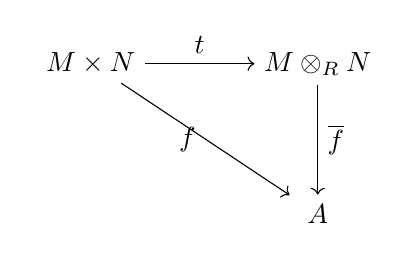
\begin{tikzpicture}
  \matrix (m) [matrix of math nodes,row sep=4em,column sep=4em,minimum width=2em]
  {
     M\times N & M \otimes_R N \\
      & A \\};
  \path[->]
  	(m-1-1.east|-m-1-2) edge node [above] {$t$}
            node [above] {} (m-1-2)
	(m-1-2) edge node [right] {$\overline{f}$} (m-2-2)
	(m-1-1) edge node [left] {$f$} (m-2-2);
    %edge [dashed,-] (m-2-1);
	\end{tikzpicture}
\end{center}
\end{prop}

\begin{proof}
El fet que $f$ sigui $R$-equilibrada fa que la seva extensió $\mathbb{Z}$-lineal $F_{\mathbb{Z}}(M\times N)$ enviï $D$ a $0$, per tant l'existència de $\overline{f}$ ve induïda per $\overline{f}(m\otimes n) = f((m,n))$. La unicitat és conseqüència del fet que els elements de la forma $m\otimes n$ generen $M\otimes_RN$.
\end{proof}

\begin{definition}
Sigui $R$ i $S$ anells. Diem que un grup abelià additiu $M$ és un \textbf{bimòdul} si és un $R$-mòdul per l'esquerra i un $S$-mòdul per la dreta, i ha de complir $r(ms)=(rm)s$, el denotem $_R{M_S}$.
\end{definition}

\begin{prop}
 Donats tres anells $R$,$S$,$T$ i dos bimòduls $_R{M_S}$ i $_S{N_T}$, el producte tensorial sobre $S$ és un bimòdul $_R{M \otimes N}_T$. 
\end{prop}

\begin{proof}
Si $r\in R$, la funció 
\begin{eqnarray*}
f_r : M\times N &\rightarrow & M\otimes_S N\\
(m,n) & \mapsto & (rm \otimes n)
\end{eqnarray*}
és $S$-equilibrada.
\\
\hspace*{.5cm}Observem que a la definició de bimòdul anterior, demanem per definició que un bimòdul compleixi $r(ms)=(rm)s$, aquesta propietat és necessària per a que la funció anterior sigui $S$-equilibrada, en particular, és necessària per a que compleixi $f_r((ms,n))=f_r((m,sn))$. \\
\\
Per tant, usant la proposició anterior hi ha un homomorfisme de grups $\mathbb{Z}$-lineal
$$
\overline{f}_r: M \otimes_S N \rightarrow M \otimes_S N
$$
amb $\overline{f}_r(m\otimes n)=(rm) \otimes n$, per $m\in M$ i $n\in N$. Observem que la funció
\begin{eqnarray*}
R\times(M\oplus_SN) & \rightarrow M & \otimes_S N \\
(r.x) & \mapsto & r \cdot x = \overline{f}_r(x)
\end{eqnarray*}
és el producte per escalars que dóna estructura de $R$-mòdul per l'esquerra a $M\otimes_S N$, ja que com que $\overline{f}_r$ és $\mathbb{Z}$-lineal i

\begin{eqnarray*}
(r+r')\cdot (m\otimes n) &=& ((r+r')m \otimes n)) = (rm+r'm \otimes n)=(rm \otimes n) + (r'm \otimes n),\\
(rr')\cdot (m\otimes n) &=&r\cdot (r' \cdot  (m\otimes n)),\\
1\cdot(m\otimes n) &=& m\otimes n
\end{eqnarray*}
Sota el producte per escalars, tenim
$$
r \cdot \sum_i^k (m_i \otimes n_i) = \sum_{i=1}^{k}(rm_i)\otimes n_i
$$
Similarment, $M\otimes_S N$ és un $T$-mòdul per la dreta via 
$$
\left( \sum_{i=1}^k (m_i\otimes n_i) \right) \cdot t = \sum_{i=1}^k m_i \otimes (n_i t)
$$
Finalment per a provar que $M \otimes_S N$ és un $R,T$-bimòdul, només cal veure que 
$$
r\cdot \left(\sum (m_i \otimes n_i) \cdot t \right) = \sum (rm_i) \otimes (n_it) = (r\cdot \sum (m_i \otimes n_i)) \cdot t.
$$
\end{proof}


%https://en.wikipedia.org/wiki/Tensor_product_of_modules#Properties
\section{La propietat IBN}

Tot espai vectorial sobre un cos té una base, i dues bases del mateix espai vectorial tenen sempre el mateix nombre d'elements, per tant el concepte de dimensió d'un espai vectorial $V$ està ben definit. A més la dimensió és un invariant que classifica els espais vectorials. \\
Hom podria pensar que aquest resultat es manté al generalitzar el concepte d'espai vectorial sobre un cos a espai vectorial sobre un anell, i.e., sobre $R$-mòduls, però no és així.\\
\indent En un $R$-mòdul $M$, l'existència d'una base no està garantida, i en cas de tenir base, podem tenir bases amb diferent cardinal, i.e., el cardinal de la base no és un invariant. L'objectiu d'aquesta subsecció és comprovar aquests fets.
\\\\
\indent La millor forma de provar que l'existència de la base no està garantida és trobar un $R$-mòdul que no tingui base.
\begin{prop}
Els grup additiu format pels racionals $\mathbb{Q}$ és un $\mathbb{Z}$-mòdul sense base.
\end{prop}
\begin{proof}
En primer lloc observem $\mathbb{Q}$ no és un $\mathbb{Z}$-mòdul cíclic, i.e., no pot estar generat per un únic element. D'altra banda, observem que dos elements qualsevols de $\mathbb{Q}$ són $\mathbb{Z}$-linealment dependents, ja que donats $m,n\in \mathbb{Q}$, existeixen $a,b\in \mathbb{Z}$ tal que es forma una combinació $\mathbb{Z}$-lineal amb $am+bn=0$. \\
Així doncs aquest $\mathbb{Z}$-mòdul no pot tenir una base formada per un element, ni una base formada per més d'un element.
\end{proof}

\begin{definition}
Diem que un anell $R$ compleix la propietat \textbf{IBN} (\textbf{I}nvariant \textbf{B}asis \textbf{N}umber) si per a tot $R$-mòdul $M$, tota parella de bases de $M$ té el mateix cardinal, és a dir, el nombre d'elements bàsics és invariant.
\end{definition}

Veiem ara que el cardinal de la base no és un invariant sobre $R$-mòduls, en particular trobarem un anell sense la propietat IBN, i.e. un $R$-mòdul amb dues bases de cardinal diferent.

\begin{prop}
El cardinal de la base no és un invariant sobre tot $R$-mòdul, amb $R$ anell no necessàriament commutatiu.
\end{prop}
\begin{proof}
Per a qualsevol $R$ anell no trivial, considerem $A$ com el conjunt de matrius definides sobre $R$ amb infinites files i columnes, tals que cada columna tingui un nombre finit d'entrades diferents de zero. \\
Observem que la suma i producte habitual doten $A$ amb l'estructura d'anell. A més, si considerem el conjunt de columnes d'elements de $A$, tenim un $A$-mòdul. En concret si $A\in A$, la columna $j$-èssima de $A$ la denotarem per $ae_j$, al considerar $A$ com a $A$-mòdul tenim que la suma i el producte són calculats per columnes:
\begin{eqnarray*}
(a+b)e_j&=ae_j+be_j \\
(ab)e_j &= a(b e_j)
\end{eqnarray*}

Així doncs tenim que $A$ és un $A$-mòdul. Per una banda observem que a la matriu identitat, denotada per 
$$1_{A}=\begin{bmatrix}
1  & 0 & \hdots  \\
0  & 1 & \hdots \\
\vdots & \vdots & \ddots
\end{bmatrix}, 
$$
és una base de $A$, i.e., $A$ té una base formada per un element. \\
\indent D'altre banda, per a cada $a\in A$, definim $a', a''$ de forma que les columnes de $a'$ siguin les columnes senars de $a$, i les columnes de $a''$ siguin les columnes parells de $a$. \\
Aleshores la funció $f: A \rightarrow A \oplus A$ definida per $f(a)=(a', a'')$ és un isomorfisme $A$-lineal amb inversa formada per ajuntar les columnes de $a'$ i $a''$. \\
Usant el fet que la imatge d'elements bàsics és element bàsic, podem veure el resultat al Corol·lari \ref{corol1}, tenim que $A$ té una base formada per dos elements

$$
f^{-1}(1_A,0_A)=\begin{bmatrix}
1  & 0 & 0 & 0 & \hdots  \\
0  & 0 & 1 & 0 & \hdots \\
\vdots & \vdots & \vdots & \vdots & 
\end{bmatrix}
, \hspace{1cm}
f^{-1}(0_A,1_A)=\begin{bmatrix}
0  & 1 & 0 & 0 & \hdots  \\
0  & 0 & 0 & 1 & \hdots \\
\vdots & \vdots & \vdots & \vdots & 
\end{bmatrix}
$$
\end{proof}


Finalment veurem que tot $R$ anell commutatiu no trivial  compleixen la propietat IBN, per a veure aquest resultat veiem el següent Lema.

\begin{lemma}
Sigui $R$ un anell commutatiu i siguin $m,n$ dos enters qualsevols tals que $m<n$, si hi ha una aplicació lineal exhaustiva $R^m \rightarrow R^n$. Aleshores $1_R=0_R$.
\end{lemma}
\begin{proof}
Sigui $\varphi$ l'aplicació exhaustiva que envia $R^m \rightarrow R^n$. L'exhaustivitat de $\varphi$ garanteix l'existència d'una aplicació $\psi$ \textit{(inversa per la dreta)} tal que $\varphi \circ \psi = \id$. Podem extendre $\varphi$ a $R^n = R^m \oplus R^{n-m}$ de forma que $\varphi(R^{n-m})=0_R$, i considerar $\psi$ com una aplicació sobre $R^n$. \\
Considerem ara les matrius $A$ i $B$ associades a les aplicacions $\varphi$ i $\psi$ respectivament. Per una banda tenim que $\det (AB) = 1_R$, d'altre banda tenim que $ \det (B)=0$ ja que la darrera fila de $B$ és plena de $0_R$'s per construcció. \\ Usant la propietat $\det(AB)=\det(A)\det(B)$ obtenim el resultat que buscàvem.
\end{proof}
Observem que a la prova anterior hem pogut usar l'existència del determinant gràcies al fet que $A$ i $B$ són matrius definides sobre un anell commutatiu.

\begin{corollary}
Si $R$ és un anell commutatiu no trivial, compleix la propietat IBN, i.e., els $R$-m.ll.f.g. tenen un nombre d'elements bàsics invariant. \footnote{Usem l'abreviatura per $R$-mòdul lliure finitament generat ($R$-m.ll.f.g.).}
\end{corollary}


%%%%%%%%%%%%%%%%%%%%%%%%%%%%%%%%%%%%%%%%%%%%%%%%%%%%%%%%%%%%%
%%%%%%%%%%%%%%%%%%%%%%MÒDULS PROJECTIUS%%%%%%%%%%%%%%%%%%%%%%
%%%%%%%%%%%%%%%%%%%%%%%%%%%%%%%%%%%%%%%%%%%%%%%%%%%%%%%%%%%%%

\section{Mòduls projectius}

Els mòduls projectius tenen un rol fonamental en la construcció de $K_0$, en aquesta secció introduïm la definició dels mòduls projectius i provem la caracterització fonamental dels mòduls projectius usant la suma directa.

\begin{definition}
 Donat un anell $R$, anomenem \textbf{mòdul projectiu sobre $R$} a un $R$-mòdul $P$ si compleix que, per a tot homomorfisme de $R$-mòduls exhaustiu $\alpha: M \twoheadrightarrow P$ existeix un homomorfisme $\beta: P \rightarrow M$ tal que $\alpha \circ \beta = id_P$, és a dir, tot homomorfisme de $R$-mòduls exhaustiu té una inversa per la dreta.
\end{definition}

%%%%%%%%%%%%%%%%%%%%%%%%%%%%%%%%%%%%%%%%%%%%%%%%%%%%%%%%%%%%%
\begin{lemma}
Un $R$-mòdul $P$ és projectiu si i només si tot diagrama de $R$-mòduls com el de la Figura \ref{DR-M} amb $\psi$ exhaustiva
%---------------------------------------------------
\begin{figure}[!htb]
\minipage{0.32\textwidth}
\begin{flushright}
 	\begin{tikzpicture}
  \matrix (m) [matrix of math nodes,row sep=3em,column sep=4em,minimum width=2em]
  {
      & P \\
     M & N \\};
  \path[->>]
    (m-2-1.east|-m-2-2) edge node [below] {$\psi$}
            node [above] {} (m-2-2);
    \path[->](m-1-2) edge node [right] {$\phi$} (m-2-2);
   % \draw[dashed,->] (m-1-2) -- (m-2-1);
\end{tikzpicture}
\caption{}
\label{DR-M}
\end{flushright}
\endminipage\hfill
\minipage{0.32\textwidth}
\textit{es pot completar fent-lo commutatiu, i.e., existeix una aplicació $\theta$ tal que} 


\endminipage\hfill
\minipage{0.32\textwidth}%
	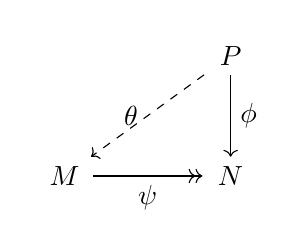
\begin{tikzpicture}
  \matrix (m) [matrix of math nodes,row sep=3em,column sep=4em,minimum width=2em]
  {
      & P \\
     M & N \\};
 \path[->>]
    (m-2-1.east|-m-2-2) edge node [below] {$\psi$}
            node [above] {} (m-2-2);
    \path[->](m-1-2) edge node [right] {$\phi$} (m-2-2);
   \draw[dashed,->] (m-1-2) edge node [left] {$\theta$} (m-2-1);
\end{tikzpicture}
\endminipage
\end{figure}
%--------------------------------------------------
\end{lemma}
%%%%%%%%%%%%%%%%%%%%%%%%%%%%%%%%%%%%%%%%%%%%%%%%%%%%%%%%%%%%%%%%%%%%%%%%%

\begin{proof} Suposem que es compleix la propietat de completació de diagrames, sigui $\alpha$ un  homomorfisme exhaustiu de $R$-mòduls $\alpha: M\rightarrow P$, hem de veure que té una inversa per la dreta. podem prendre $N=P$, $\phi = id_P$, i $\psi = \alpha$. Aleshores el $\theta:P \rightarrow M$ resultant de la propietat de completació de diagrames compleix $\alpha \circ \theta = id_P$, i.e. $\beta$ és la inversa per la dreta de $\alpha$.
\\
\indent Veiem ara el recíproc, suposem que tot homomorfisme de $R$-mòduls exhaustiu $\alpha : M \rightarrow P$ té una inversa per la dreta $\beta : P \rightarrow M$. Donat un diagrama de $R$-mòduls com el de la Figura \ref{DR-M} , canviant $M \xrightarrow{\psi} N$ per $M \oplus P \xrightarrow{\psi \oplus id_P} N \oplus P$ i $\phi:P\rightarrow N$ per $((\phi, id_P):P \rightarrow N\oplus P)$, podem suposar que $\phi$ és injectiva (Figura \ref{finj}). A més, si canviem $N$ per la imatge de $\phi$ i $M$ per $\psi^{-1}(\phi(P))$, podem suposar que $\phi$ és un isomorfisme (Figura \ref{fbij}). Aleshores, considerant $\beta$ com la inversa per la dreta de $\alpha = \phi^{-1} \circ \psi$ tenim que $\beta : P \rightarrow M$ ens permet completar el diagrama.






%------------------------------------------------
%---------------------------------------------------
\begin{figure}[!htb]
\minipage{0.22\textwidth}

\begin{center}
 	\begin{tikzpicture}
  \matrix (m) [matrix of math nodes,row sep=3em,column sep=4em,minimum width=2em]
  {
      & P \\
     M & N \\};
  \path[->>]
    (m-2-1.east|-m-2-2) edge node [below] {$\psi$}
            node [above] {} (m-2-2);
    \path[->](m-1-2) edge node [right] {$\phi$} (m-2-2);
   % \draw[dashed,->] (m-1-2) -- (m-2-1);
\end{tikzpicture}
\end{center}
\endminipage\hfill
\minipage{0.32\textwidth}
\begin{center}
	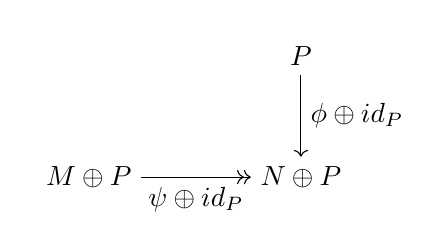
\begin{tikzpicture}
  \matrix (m) [matrix of math nodes,row sep=3em,column sep=4em,minimum width=2em]
  {
      & P \\
     M \oplus P& N \oplus P \\};
  \path[->>]
    (m-2-1.east|-m-2-2) edge node [below] {$\psi \oplus id_P$}
            node [above] {} (m-2-2);
    \path[->](m-1-2) edge node [right] {$\phi \oplus id_P$} (m-2-2);
   % \draw[dashed,->] (m-1-2) -- (m-2-1);
\end{tikzpicture}
\caption{} \label{finj}
\end{center}

\endminipage\hfill
\minipage{0.42\textwidth}%
\begin{center}
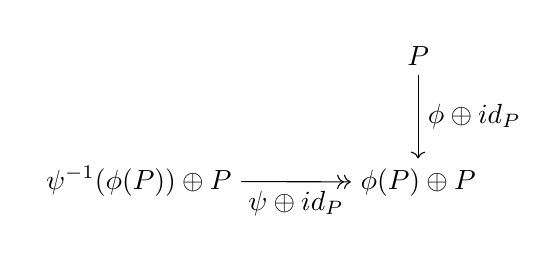
\begin{tikzpicture}
  \matrix (m) [matrix of math nodes,row sep=3em,column sep=4em,minimum width=2em]
  {
      & P \\
     \psi^{-1}(\phi(P)) \oplus P & \phi(P) \oplus P \\};
  \path[->>] (m-2-1) edge node [below] {$\psi \oplus id_P$}(m-2-2)
            node [above] {} (m-2-2);
            
   \path[->] (m-1-2) edge node [right] {$\phi \oplus id_P$} (m-2-2);
    %edge [dashed,-] (m-2-1);
\end{tikzpicture}
\caption{} \label{fbij}
\end{center}

\endminipage
\end{figure}
%--------------------------------------------------
%------------------------------------------------

\end{proof}

%%%%%%%%%%%%%%%%%%%%%%%%%%%%%%%%%%%%%%%%%%%%%%%%%%%%%%%%%%%%%%%%%%%%%%

\begin{obs}\label{sumasplit}Observem que si $\alpha : M\rightarrow P$ és exhaustiva i $\beta:P\rightarrow M$ és la seva inversa per la dreta, aleshores $p:=\beta \circ \alpha$ és un endomorfisme idempotent de $M$ ja que 
\begin{equation} 
\begin{split}
(\beta \circ \alpha)^2 & = (\beta \circ \alpha) \circ (\beta \circ \alpha) \\
 & = \beta \circ (\alpha \circ \beta) \circ \alpha \\
 &= \beta \circ id_P \circ \alpha  = \beta \circ \alpha
\end{split}
\end{equation}
A més, usant la Proposició \ref{img+ker=M} tenim que $M \cong P \oplus \text{Ker($p$)} = P \oplus (1-p)(M) $
\end{obs}

\begin{lemma}
 Sigui $R$ un anell, tot $R$-mòdul lliure és projectiu. 
\end{lemma}
\begin{proof} Sigui $F$ un $R$-mòdul lliure, al ser lliure ha de tenir una base $B$. Sigui $\alpha: M \rightarrow F$ un homomorfisme de mòduls exhaustiu,  gràcies a l'exhaustivitat de $\alpha$ per a cada element bàsic $x_i\in B \subset F$ ha d'existir algun $y_i\in M$ tal que $\alpha(y_i)=x_i$. Definim l'aplicació $\beta$ a partir de la imatge dels elements bàsics $\beta(x_i)=y_i$, usant la Proposició \ref{morfismebase} $\beta$ és un morfisme $F\rightarrow M$ ben definit. A més, és inversa per la dreta de $\alpha$.
\end{proof}

\begin{theorem}[Caracterització fonamenteal dels mòduls projectius] \label{carProj}
Sigui $R$ un anell. Un $R$-mòdul és projectiu si i només si és isomorf a un sumand directe d'un $R$-mòdul lliure\footnote{i.e. existeix un $R$-mòdul $Q$ i un $R$-mòdul lliure $F$ tal que $F = P \oplus Q$.}. És finitament generat i projectiu si i només si és isomorf a un sumand directe de $R^n$ per algun $n$.
\end{theorem}

\begin{proof}Si $P$ és un mòdul projectiu, ha de tenir almenys un conjunt generador $G$ (no és necessàriament una base de $P$). Triem un $R$-mòdul $F$ amb base $B$ que ens permeti definir una aplicació bijectiva entre elements de $B$ i $G$. Usant de nou \ref{morfismebase} tenim que $\alpha$ té una extensió a una aplicació $R$-lineal $\hat{\alpha}: F\rightarrow P$. De fet, com que la imatge de $B$ és $P$, $\hat{\alpha}$ és exhaustiva. Usant l'Observació anterior tenim que $P$ és isomorf a una suma directa en un $R$-mòdul lliure, a més, si $P$ és finitament generat, podem escollir que $F$ sigui exactament $R^n$ on $n$ és el nombre d'elements de $G$.
\\
Per a veure el recíproc, suposem que $F\cong P\oplus Q$, on $F$ és un mòdul lliure. Donat un homomorfisme de $R$-mòduls exhaustiu $\alpha : M \rightarrow P$, observem que l'homomorfisme de $R$-mòduls $\alpha \oplus id_Q:(M\oplus Q)\rightarrow (P\oplus Q)=F$ també és exhaustiu . A més, com que $F$ és lliure, ha de ser projectiu. Així doncs, usant la projectivitat de $F$ tenim que $\alpha \oplus id_Q$ té una inversa per la dreta. Si restringim la inversa per la dreta a $P$ i la projectem sobre $M$ tenim una inversa per la dreta de $\alpha$. Per acabar, si $F\cong R^n$ amb generadors $x_1,\dots, x_n \in B$, aleshores $P$ ve generat pels $n$ elements $p(x_i)$, on $p$ és la identitat a $P$ i $0$ a $Q$.
\end{proof}


% Chapter 1

\chapter{Construcció del Grup $K_0$} % Main chapter title

La dimensió és un invariant dels espais vectorials que els classifica, és a dir, dos espais vectorials sobre un cos $K$ són isomorfs si i només si tenen la mateixa dimensió, en concret podem crear una bijecció entre la col·lecció de classes d'isomorfisme de $K$-espais vectorials i $\mathbb{N}$, a més, la suma directa ens permet sumar espais vectorials, de forma que $\dim(V \oplus W) = \dim (V) + \dim (W)$. Per afegitó, podem completar el monoide $\mathbb{N}$  a un grup abelià $\mathbb{Z}$ que conté totes les diferències d'enters no negatius $m-n$. Similarment, podem completar el monoide de la col·lecció de les classes de isomorfia d'espais vectorials al grup $K_0(K)$, aquest grup és isomorf a $\mathbb{Z}$ i consisteix en les diferències $c(V)-c(W)$ on $c$ denota la classe d'isomorfisme dels espais vectorials. \\
\indent Al generalitzar el cas d'un cos $K$ a un anell arbitrari $R$ tenim que els $R$-mòduls no tenen necessàriament una base, per tant el concepte de dimensió desapareix, però si restringim la nostre atenció a la classe dels $R$-mòduls projectius, tenim que el grup abelià $K_0(R)$ segueix intacte com el fantasma desaparegut de la dimensió. L'estructura de $K_0(R)$ reflecteix la generalització del concepte de dimensió dels espais vectorials sobre $R$-mòduls. En particular si $R$ no és un cos, $K_0(R)$ no és necessàriament isomorf a $\mathbb{Z}$. \\ 
\indent En aquest capítol presentarem $K_0(R)$, començarem definint-lo a partir de classes d'isomorfisme de mòduls projectius i després usarem la relació entre mòduls projectius i els idempotents per a presentar $K_0$ a partir de classes d'equivalència de matrius idempotents. Aquestes caracteritzacions ens permetran mostrar amb facilitat propietats del grup. Després estudiem $K_0$ per a cossos, dominis d'ideals principals i anells locals. A la darrera secció introduirem el grup $K_0$ relatiu, aquest grup ens permetrà trobar una successió exacta que generalitzarem al següent capítol relacionant els grups $K_0$ i $K_1$. Finalment veurem que $K_0$ també es pot definir per a anells sense unitat.
\\
\indent La referència bibliogràfica essencial d'aquest capítol és [1], a més s'ha usat [2] com a referència puntulament, també hem usat [7]  per l'\textit{Eilenberg swindle}, [9] per el Lema de Nakayama i el seu corol·lari, i un resultat puntual de [8] que no hem provat però està explícitament referenciat durant el capítol.

\label{Chapter1} % For referencing the chapter elsewhere, use \ref{Chapter1} 

%----------------------------------------------------------------------------------------

% Define some commands to keep the formatting separated from the content 
\newcommand{\keyword}[1]{\textbf{#1}}
\newcommand{\tabhead}[1]{\textbf{#1}}
\newcommand{\code}[1]{\texttt{#1}}
\newcommand{\file}[1]{\texttt{\bfseries#1}}
\newcommand{\option}[1]{\texttt{\itshape#1}}

%----------------------------------------------------------------------------------------


\section{$K_0$ a partir de mòduls projectius}
L'objectiu d'aquesta secció és definir $K_0$ a través de mòduls projectius, en primer lloc notarem la importància de considerar el conjunt de classes d'isomorfisme de mòduls projectius en lloc de prendre la col·lecció de tots els mòduls projectius, posteriorment presentem el grup de Grothendieck i finalment definim $K_0$.
\begin{definition}
Donat un anell $R$, denotem per $\proj R$ a les classes d'isomorfisme de mòduls projectius finitament generats. 
\end{definition}
La següent Proposició justifica perquè prenem classes d'isomorfisme, però abans necessitem un Lema:
\begin{lema}
La col·lecció de tots els singletons no és un conjunt. (Un singletó és un conjunt format per un únic element).
\end{lema}
\begin{proof}
Si $A$ és un conjunt que conté tots els singletons, per l'axioma de la unió ( l'axioma de la unió afirma que per a un conjunt arbitrari $A$, existeix el conjunt $\bigcup A$ que consisteix en els elements dels elements del conjunt), $\cup A$ és un conjunt, però és el conjunt que conté tots els conjunts, per la paradoxa de Russell no pot ser un conjunt . Per tant $A$ no és un conjunt.
\end{proof}

\begin{prop}
Sigui $P$ la col·lecció de tots els $R$-mòduls projectius finitament generats, llavors $P$ no és un conjunt.
\end{prop}
\begin{proof}
Observem que donats dos elements diferents  $\bullet \neq \star$, el mòdul $(\{\bullet\},+,\cdot)$ amb estructura $\bullet+\bullet=\bullet$ i $r \cdot \bullet = \bullet$ per a tot $r\in R$; és un mòdul diferent del mòdul $(\{\star\},\oplus,\odot)$ amb estructura $\star \oplus \star = \star$ i $r\odot \star=\star$ per a tot $r\in R$.
\\
Així doncs, per cada conjunt format per un únic element (singletó), podem crear un $R$-mòdul finitament generat, i com que la col·lecció de tots els singletons no és un conjunt, la col·lecció de tots els $R$-mòduls tampoc pot ser un conjunt.
\end{proof}

Així doncs, hem de considerar $\text{Proj} \ R$ com el conjunt de classes d'isomorfia, és a dir, per a cada classe d'isomorifa escollim un, i només un, mòdul que la representi.


\begin{prop}
 $\proj R$ amb l'operació binària $\oplus$ té estructura de semigrup (un semigrup és un conjunt $S$ junt amb una operació binària associativa $\cdot: S \times S \rightarrow S$). 
\end{prop}
\begin{proof}
Si $P,Q \in \proj R$, al ser $R$-mòduls projectius finitament generats existeixen dos $R$-mòduls $P',Q'$ i dos enters positius $n,m$ tal que $P\oplus P' \cong R^m$ i $Q \oplus Q' \cong R^n$. Aleshores usant que $\oplus$ és associativa tenim
$$
(P\oplus Q) \oplus (P' \oplus Q') \cong (P \oplus P') \oplus (Q \oplus Q') \cong R^m \oplus R^n \cong R^{n+m}
$$
Observem que la suma directa està ben definida, ja que si $P\cong P'$ i $Q\cong Q'$, aleshores $P\oplus Q \cong P' \oplus Q'$. \\
De fet, $\proj R$ té estructura de monoide, ja que té per element identitat el mòdul $0$. 
\end{proof}
Tenim doncs que $\proj R$ té estructura de semigrup, però en general no té estructura de grup. El següent Teorema ens permet forçar l'estructura de grup a $\proj R$. La idea que ens permetrà dotar d'estructura de grup és una generalització de la construcció del grup abelià additiu $\mathbb{Z}$ a partir dels enters positius, o de la construcció de $\mathbb{Q}^\times$ a partir dels enters no nuls, consisteix a introduir inverses formals per a certs elements.

\begin{theorem} \label{GG} Sigui $S$ un semigrup commutatiu (sense necessitat de tenir element unitat). Existeix un grup abelià $G$, anomenat \textbf{grup de Grothendieck} o grup completat de $S$, junt amb un homomorfisme de semigrups $\varphi: S \rightarrow G$, tal que per a tot grup $H$ i tot homomorfisme $\psi : S \rightarrow H$, hi ha un únic homomorfisme $\theta: G\rightarrow H$ amb $\psi = \theta \circ \varphi$.




\begin{figure}[!htb]
\minipage{0.32\textwidth}
\begin{flushright}
	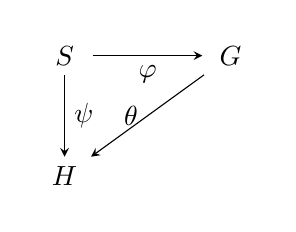
\begin{tikzpicture}
  \matrix (m) [matrix of math nodes,row sep=3em,column sep=4em,minimum width=2em]
  {
     S & G \\
     H &  \\};
  \path[-stealth]
  	(m-1-1.east|-m-1-2) edge node [below] {$\varphi$}
            node [above] {} (m-1-2)
	(m-1-1) edge node [right] {$\psi$} (m-2-1)
	(m-1-2) edge node [left] {$\theta$} (m-2-1);
    %edge [dashed,-] (m-2-1);
	\end{tikzpicture}
\end{flushright}
\endminipage\hfill
\minipage{0.32\textwidth}
\textit{La unicitat es compleix en el sentit que si $\varphi ': S\rightarrow G'$ és una altra parella amb la mateixa propietat, aleshores existeix un isomorfisme $\alpha: G \rightarrow G'$ amb $\varphi ' = \alpha \circ \varphi$.}


\endminipage\hfill
\minipage{0.32\textwidth}%
		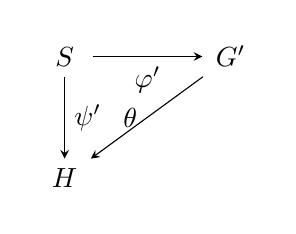
\begin{tikzpicture}
  \matrix (m) [matrix of math nodes,row sep=3em,column sep=4em,minimum width=2em]
  {
     S & G' \\
     H &  \\};
  \path[-stealth]
  	(m-1-1.east|-m-1-2) edge node [below] {$\varphi '$}
            node [above] {} (m-1-2)
	(m-1-1) edge node [right] {$\psi '$} (m-2-1)
	(m-1-2) edge node [left] {$\theta$} (m-2-1);
    %edge [dashed,-] (m-2-1);
	\end{tikzpicture}
\endminipage
\end{figure}
\end{theorem}

\begin{proof}
Definim $G$ com el conjunt de les classes d'equivalència de parelles $(x,y)$ amb $x,y\in S$, on $(x,y) \sim (u,v)$ si i només si hi ha un $t\in S$ tal que 
$$
x+v+t = u+y+t \ \text{ a } S .
$$
Denotem per $ [(x,y)] $ a la classe d'equivalència de $(x,y)$. Aleshores definim la suma per
$$
[(x,y)]+[(x',y')]=[(x+x',y+y')]
$$
La suma de classes està ben definida, ja que si $(x,y)\sim (u,v)$,  i $(x',y') \sim (u',v')$ aleshores existeixen $t,t' \in S$ tal que 
\begin{eqnarray*}
\begin{cases}
x+v+t&=y+u+t \\ 
x'+v'+t'&=y'+u'+t'
\end{cases}
\Rightarrow 
x+x'+v+v'+t+t'=y+y'+u+u'+t+t'
\end{eqnarray*}
 Al ser $S$ un semigrup, $t+t'\in S$ i per tant
 $$(x,y)+(x',y')=(x+x',y+y')\sim (u+u',v+v') = (u,v)+(u',v').$$
\noindent Com que l'associativitat se segueix complint, tenim que $G$ amb la suma té estructura de semigrup. A més, com que $S$ és commutatiu tenim que $x+y=y+x$ i per tant $[(x,x)]=[(y,y)]$, observem que aquest element és element neutre de $G$, i.e., $0_G$. De fet aquest element dóna estructura de monoide a $G$.
També es compleix que tot element de $G$ té invers:
$$
[(x,y)]+ [(y,x)] = [(x+y,x+y)] = 0,
$$
per tant $G$ és un grup. Definim $\varphi: S\rightarrow G$ com
$$
\varphi(x)=[(x+x,x)]
$$
es compleix $\varphi(x)+\varphi(y)=\varphi(x+y)$, per tant és un homomorfisme de semigrups. 
\\ Observem que la imatge de $\varphi$ genera $G$ com a grup ja que 
$$
[(x,y)]=\varphi(x)-\varphi(y)
$$
 Donat un grup $H$ i un homomorfisme $\psi: S\rightarrow H$, el homomorfisme $\theta: G\rightarrow H$ amb $\psi = \theta \circ \phi$ es defineix per
$$
\theta([(x,y)])=\psi(x)-\psi(y).
$$
\indent  Una manera alternativa de definir $G$ és definir-lo com el grup generat per $[x]$, amb $x\in S$, sota la relació $[x]+[y]=[z]$ a $G$ si $x+y=z$ a $S$. Observem que $[(x,y)]$ de la construcció anterior correspon a $[x]-[y]$ d'aquesta relació. L'aplicació $\varphi$ és $x\mapsto [x]$, i tot homomorfisme de $S$ a un grup $H$ ha de factoritzar a través de $G$ per construcció. \\

Per provar la unicitat, suposa que $\varphi '  :  S \rightarrow G'$ té la mateixa propietat universal. En primer lloc, $\varphi ' (S)$ ha de generar $G'$ ja que, en cas contrari, si $G''$ és el subgrup generat per la imatge de $\varphi ' $, aleshores hi ha dos homomorfismes $\theta : G' \rightarrow G' \oplus G'/G''$ amb
$$
(\varphi ',0) = \theta \circ \varphi ' 
$$
aquests són $\theta = (id,0)$ i $\theta = (id,q)$ on $q$ és la projecció canònica. \\
Aplicant la propietat universal per a $G$ i $G'$, han d'existir aplicacions $\alpha :  G \rightarrow G'$ amb  $\varphi ' = \alpha \circ \varphi$ i $\beta: G'\rightarrow G$ amb  $\varphi = \beta \circ \varphi '$. 
A més $\alpha \circ \beta = id$ a la imatge de $\varphi'$, i.e., a tot $G'$, i per tant té inversa per l'esquerra $\beta$. Similarment $\beta \circ \alpha = id$ a la imatge de $\varphi$, per tant també tenim que $\alpha$ és inversa per la dreta de $\beta$.
 \end{proof}
 \begin{obs}
 L'assignació $S \leadsto G=G(S)$ és de fet un functor de la categoria de semigrups abelians a la categoria de grups abelians, ja que si $\gamma: S \rightarrow S'$ és un homomorfisme de semigrups, indueix un diagrama commutatiu
\begin{center}
		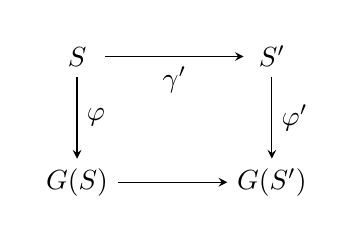
\begin{tikzpicture}
  \matrix (m) [matrix of math nodes,row sep=3em,column sep=4em,minimum width=2em]
  {
     S & S' \\
     G(S) & G(S')  \\};
  \path[-stealth]
  	(m-1-1.east|-m-1-2) edge node [below] {$\gamma '$}
            node [above] {} (m-1-2)
	(m-1-1) edge node [right] {$\varphi$} (m-2-1)
	(m-1-2) edge node [right] {$\varphi '$} (m-2-2)
	(m-2-1.east|-m-2-2) edge node [below] {}
            node [above] {} (m-2-2);
    %edge [dashed,-] (m-2-1);
	\end{tikzpicture}
\end{center}
 on l'aplicació $G(S)\rightarrow G(S')$ és unívocament determinada per la propietat universal de G(S) que acabem de demostrar.
 

\end{obs}
\begin{obs}
 L'aplicació $\varphi: S \rightarrow G$ (en el context del Teorema \ref{GG}) és injectiva si i només si la propietat cancel·lativa es compleix a $S$, i.e. $(x+z=y+z \Rightarrow x=y)$ per a tot $x,y,z\in S$
\footnote{
Si tenim $x,y\in S$ elements diferents tals que $[x+x,x]=[y+y,y]$, aleshores $x+x+y=y+y+x$, si prenem $z=x+y$ tenim $x+z=y+z$ però per hipòtesi $x\neq y$, per tant no es compleix la propietat cancel·lativa. Podem invertir el raonament per veure el recíproc.}. Els semigrups sense propietat cancel·lativa són generalment difícils de tractar, en canvi tractar el seus grup de Grothendieck pot ser més senzill.
 \end{obs}

Veiem ara un exemple de càlcul específic del grup de Grothendieck d'un semigrup específic. \\
\textup{\textbf{Exemple.}
Sigui $S$ el monoide abelià amb elements $a_{n,m}$, on $n\in \mathbb{N}$, i
$$
\begin{cases}
m=0 \ \text{ si } n=0 \ \text{o} \  1\\
m\in \mathbb{Z} \ \text{ si } \  n=2 \\
m\in \mathbb{Z}/2 \ \text{ si } \ n\geq 3
\end{cases}
$$
amb l'operació de semigrup donada per la fórmula
$$
a_{n,m}+a_{n',m'}=a_{n+n',m+m'}
$$
on $m+m'$ es calcula a $\mathbb{Z}$ si $n+n' \leq 2$ ia $\mathbb{Z}/2$ si $n+n' \geq 3$. \\
\indent Per calcular el grup de Grothendieck $G(S)$ del monoide, nota primer que $\varphi$ no és injectiva, ja que per $m,n\in \mathbb{Z}$ amb $m \equiv n\ (2)$ i $m\neq n$, compleix que $\varphi((2,n))=\varphi((2,m))$. Així doncs usant l'observació anterior tenim que la propietat cancel·lativa a $S$ no es compleix. \\
Usarem que $G(S)$ ve generat per $\varphi(S)$, per tant convé calcular
\begin{eqnarray*}
\varphi:&S & \rightarrow  G(S)\\
&(0,0) & \mapsto  [(0,0),(0,0)] \sim (0,0) \\
&(1,0) & \mapsto  [(2,0),(1,0)] \sim (1,0) \\
&(2,n) & \mapsto  [(4,2n),(2,n)] \sim (2,n \ \text{mod} \ 2) \\
&(m,0) & \mapsto  [(2m,0),(m,0)] \sim (m,0) \\
&(m,1) & \mapsto  [(2m,2),(m,1)] \sim (m,1)
\end{eqnarray*}
per $n,m\in \mathbb{Z}$ i $m \geq 3$. Tenim doncs que aquests elements formen el grup $$G(S)\cong\mathbb{Z}\times \mathbb{Z}/2\mathbb{Z}.$$
}

\begin{definition} Sigui $R$ un anell amb unitat. Aleshores $K_0(R)$ és el \textbf{grup de Grothendieck} (en el mateix sentit que en el Teorema \ref{GG}) del semigrup $\proj R$ (semigrup format per classes d'isomorfisme de $R$-mòduls projectius finitament generats).
\end{definition}

Podríem provar que $K_0$ és un \textbf{functor}, en el sentit que si $\varphi: R \rightarrow R'$ és un homomorfisme d'anells, hi ha un homomorfisme induït $K_0(\varphi)=\varphi_*:K_0(R)\rightarrow K_0(R')$, aquest fet esdevindrà trivial a partir de la caracterització dels mòduls projectius a través de classes de matrius idempotents.

\section{$K_0$ a partir d'idempotents.}
L'objectiu d'aquesta secció és caracteritzar el grup $K_0$ a partir de les classes d'equivalència d'idempotents, en lloc de fer-ho a partir de les classes d'isomorfia de mòduls projectius com hem fet a la secció anterior. Aquesta caracterització ens facilitarà provar propietats rellevants per al càlcul de $K$-grups. 

\indent Si $P$ és $R$-m.p.f.g,\footnote{Usem l'abreviatura $R$-m.p.f.g. per a referir-nos a $R$-mòduls projectius finitament generats.} usant la caracterització dels mòduls projectius (Teorema \ref{carProj}) podem assumir sota isomorfisme que $P\oplus Q = R^n$ per algun $n$, a més per la Proposició \ref{primer}  existeix automorfisme de $R$-mòduls idempotent sobre $R^n$ que consisteix per ser la identitat sobre $P$ i 0 sobre $Q$. Si a més tenim en compte que tot homomorfisme de $R$-mòduls $R^n\rightarrow R^n$ ve determinat per la imatge dels $n$ vectors bàsics, aquest homomorfisme es correspon a una matriu $n\times n$ que actua per la dreta. Per tant, el mòdul projectiu $P$ queda determinat per una matriu idempotent $p$ de dimensions $n\times n$.
\\
\indent
No obstant hi ha matrius idempotents diferents que poden donar lloc a la mateixa classe de mòduls projectius.
Per exemple en el cas d'un cos l'únic invariant d'un mòdul projectiu és la seva dimensió, que es correspon amb el rang de $p$.\\
Per tant, si pretenem caracteritzar $K_0(R)$ a partir de matrius idempotents, és indispensable descriure una relació d'equivalència entre les matrius idempotents de forma que cada classe de matrius idempotents es correspongui a una i només una classe de mòduls projectius.

\begin{lema}
Si $p$ i $q$ són matrius idempotents, possiblement de diferents mides, sobre un anell $R$; els corresponents $R$-m.p.f.g. són isomorfs si i només si podem augmentar la mida de les matrius $p$ i $q$ afegint zeros a la cantonada inferior-dreta de forma que tinguin la mateixa mida $N\times N$ i siguin conjugades sota el grup $GL(N,R)$ de matrius $N\times N$ invertibles sobre $R$. 
\end{lema}

\begin{proof}
Si $u\in GL(N,R)$ i $upu^{-1}=q$, aleshores el producte per la dreta indueix un isomorfisme de $R^Nq$ a $R^Np$, per tant la condició és suficient. Per a provar que la condició és necessària suposem que $p$ i $q$ són matrius de mida $n\times n$ i $m\times m$ respectivament, i que $R^np \cong R^mq$. Podem extendre aquest isomorfisme $\alpha : R^np\rightarrow R^mq$ a un homomorfisme de $R$-mòduls $R^n \rightarrow R^m$ a partir de prendre $\alpha =0$ en el complementari del mòdul $R^n(1-p)$, i veure la imatge de $R^mq$ incrustada a $R^m$. Similarment extenem $\alpha^{-1}$ a un homomorfisme de $R$-mòduls $\beta : R^m \rightarrow R^n$ el qual pren valors 0 sobre $R^m(1-q)$.
Aleshores $\alpha$ ve donada per la multiplicació per la dreta per una matriu $\alpha$ d mida $n\times m$ i $\beta$ ve donada per multiplicar per la dreta per una matriu $b$ de mida $m\times n$. A més, tenim les relacions $ab=p, ba=q, a=pa=aq, b=qb=bp$. La gràcia de la prova consisteix en prendre $N=n+m$ i notar que 
$$
\left( \begin{matrix}
  1-p & a \\
  b & 1-q
 \end{matrix} \right)^2
 =
 \left( \begin{matrix}
  1 & 0 \\
  0 & 1
 \end{matrix} \right)
$$
complint la conjugació
$$
\left( \begin{matrix}
  1-p & a \\
  b & 1-q
 \end{matrix} \right)
 \left( \begin{matrix}
  p & 0 \\
  0 & 0
 \end{matrix} \right)
 \left( \begin{matrix}
  1-p & a \\
  b & 1-q
 \end{matrix} \right)
 =
 \left( \begin{matrix}
  1-p & a \\
  b & 1-q
 \end{matrix} \right)
 \left( \begin{matrix}
  0 & a \\
  0 & 0
 \end{matrix} \right)
 =
  \left( \begin{matrix}
  0 & 0 \\
  0 & q
 \end{matrix} \right) .
$$
per tant $\left( \begin{matrix}
  1-p & a \\
  b & 1-q
 \end{matrix} \right)$ és una matriu de $GL(N,R$)que conjuga $p\oplus 0$ amb $0\oplus q$, finalment i per acabar observem que $0\oplus q$ és conjugat de $q\oplus 0$ a partir de la matriu permutació.
\end{proof}

Ara estem en condicions de descriure $\proj R$.

\begin{definition} \label{incrustacio}
Sigui $R$ un anell, deontem $M(n,R)$ a la col·lecció de matrius $n\times n$ sobre un anell $R$ i $GL(n,R)$ al grup de matrius invertibles $n\times n$ sobre $R$. Incrustem $M(n,R)$ a $M(n+1,R)$ a partir de $a \mapsto
 \left( \begin{matrix}
  a & 0 \\
  0 & 0
 \end{matrix} \right)$ i incrustem $GL(n,R)$ a $GL(n+1,R)$ a partir de l'homomorfisme de grups
  $a \mapsto 
 \left( \begin{matrix}
  a & 0 \\
  0 & 1
 \end{matrix} \right)$.
 Denotem per $M(R)$ i $GL(R)$ la unió infinita dels grups $M(n,R)$ i $GL(n,R)$ respectivament, observem que tota matriu d'aquests grups té una mida finita. Denotarem $\idem R$ al conjunt de matrius idempotents a $M(R)$, a més, observem que $GL(R)$ actua a $\idem R$ per conjugació com hem vist al Lema anterior.
\end{definition}

\begin{theorem}
Per a tot anell $R$, podem identificar $\proj R$ com el conjunt d'òrbites de l'acció de $GL(R)$ a $\idem R$. L'operació de semigrup és induïda per 
$
(p,q)\mapsto 
 \left( \begin{matrix}
  p & 0 \\
  0 & q
 \end{matrix} \right) .
$
Per tant $K_0(R)$ és el grup de Grothendieck d'aquest semigrup.
\end{theorem}

Per acabar veiem que $K_0$ és invariant sota el pas de $R$ a $M_n(R)$ i un Corol·lari del Teorema anterior que ens serà molt útil per a calcular $K$-grups.

\begin{theorem}[Invariància de Morita]
Per a tot anell $R$ i tot enter positiu $n$ hi ha un isomorfisme natural 
$$K_0(R)\leftrightarrow K_0(M_n(R)).$$
\end{theorem}
\begin{proof}
Usant la identificació $M_k(M_n(R))$ amb $M_{kn}(R)$, tenim que 
$$
\idem (M_n(R)) = \idem (R) \ \text{i} \ GL(M_n(R)) = GL(R).
$$
Per tant aquest resultat és un corol·lari del Lema anterior.
\end{proof}

\begin{cor} \label{K0Cartesian}
Donats dos anells $R_1$ i $R_2$,
$$
K_0(R_1\times R_2) \cong K_0(R_1) \oplus K_0(R_2).
$$ 
\end{cor}
\begin{proof}
Usant la identificació $M_{2n}(R)$ amb $M_{n}(R)\times M_n(R)$ tenim que
$$\idem(R_1\times R_2) = (R_1) \times \idem (R_2)$$, a més, $GL(R_1\times R_2) = GL(R_1)\times GL(R_2)$ actua per conjugació sobre aquest semigrup, per tant $\proj (R_1\times R_2) \cong \proj R_1 \times \proj R_2$, i per tant $$K_0(R_1\times R_2) \cong K_0(R_1) \oplus K_0(R_2).$$ Aquest raonament es pot generalitzar per a productes finits.
\end{proof}
%%%%%%%%%%%%%%%%%%%%%%%%%%%%%%%%%%%%%%%%%%%%%%%%%%%
%%%%%%%%%%%%%%%%%%%%%%%%%%%%%%%%%%%%%%%%%%%%%%%%%%%
%%%%%%%%%%%%%%%%%%%%%%%%%%%%%%%%%%%%%%%%%%%%%%%%%%%
%%%%%%%%%%%%%%%%%%%%%%%%%%%%%%%%%%%%%%%%%%%%%%%%%%%
%%%%%%%%%%%%%%%%%%%%%%%%%%%%%%%%%%%%%%%%%%%%%%%%%%%
\section{El cas d'un cos}
En aquesta secció estudiarem $K_0$ sobre un cos i notarem el motiu pel qual restringim la definició de $K_0$ sobre mòduls projectius finitament generats.
\begin{prop}
 Si $R$ és un cos, $K_0(R)\cong \mathbb{Z}$.
\end{prop}
\begin{proof}
Si $R$ és un cos tot $R$-m.p.f.g. és un $R$-espai vectorial, i per tant té una base i una dimensió ben definides. De fet, la dimensió és l'únic isomorfisme invariant del mòdul, per tant tenim $\proj R \cong \mathbb{N}$, considerat com el monoide additiu dels nombres naturals. Com que la compleció (grup de Grothendieck) del semigup $\mathbb{N}$ és $\mathbb{Z}$, tenim $K_0(R)\cong \mathbb{N}$.
\end{proof}
\begin{obs}
El mateix argument de la prova anterior mostra que $K_0(R)\cong \mathbb{Z}$ si $R$ és un anell de divisió.
\end{obs}
\begin{obs}
Si $R$ és un cos i en lloc de calcular el grup de Grothendieck de $\proj R$ calculem el grup de Grothendieck del monoide format per les classes d'isomorfisme dels mòduls projectius \textbf{numerablement generats}, amb el mateix argument que el de la prova anterior tenim que aquest monoide és isomorf a $\mathbb{N} \cup \infty$, amb la norma habitual $n+\infty = \infty$ per a tot $n$. Observem en aquest monoide no es compleix la propietat cancel·lativa, de fet dos elements qualsevols esdevenen isomorfs si sumem $\infty$ a cada banda. Per tant el grup de Grothendieck d'aquest monoide és trivial. Així doncs és raonable usar només mòduls \textbf{finitament generats} per definir $K_0$.
\end{obs}

De fet podem generalitzar l'observació anterior sobre un anell $R$ qualsevol.

\begin{prop}["Eilenberg swindle"]
Si $R$ és un anell, el grup de Grothendieck del semigrup de les classes d'isomorfia dels $R$-mòduls projectius numerablement generats desapareix, i.e., és trivial.
\end{prop}

\begin{proof}
Si $R^\infty$ és un mòdul lliure infinitament generat numerablement i $P$ és un mòdul projectiu tal que $P\oplus Q \cong R^n$,  per commutativitat de la suma directa es compleix $Q \oplus P \cong R^n$. Així doncs tenim 
\begin{eqnarray*}
P\oplus R^\infty  \cong  P\oplus(Q\oplus P) \oplus (Q \oplus P) \dots 
 \cong  (P \oplus Q) \oplus (P \oplus Q) \dots 
\cong  R^\infty .
\end{eqnarray*}
A més si $P\oplus R^m \cong R^\infty$, amb $m\neq \infty$, aleshores $P\cong R^\infty$. També es compleix la propietat $R^\infty \cong R^\infty \oplus R^\infty$. \\
Així doncs, $P\oplus R^\infty \cong R^\infty \oplus R^\infty$ implica que per a qualsevol parella d'elements del semigrup existeix un element $(R^{\infty})$ que els fa isomorfs, per tant el grup de Grothendieck ha de ser trivial.
\end{proof}




%%%%%%%%%%%%%%%%%%%%%%%%%%%%%%%%%%%%%%%%%%%%%%%%%%%
%%%%%%%%%%%%%%%%%%%%%%%%%%%%%%%%%%%%%%%%%%%%%%%%%%%
%%%%%%%%%%%%%%%%%%%%%%%%%%%%%%%%%%%%%
\section{El cas dels DIPs}
En aquesta secció estudiarem $K_0$ sobre un domini d'ideals principals, en particular veurem que té sentit el concepte de dimensió en els $R$-mòduls sobre DIPs, i presentarem el grup $K_0$ reduït.

\begin{definition}{} Un $DIP$ (\textbf{domini d'ideals principals}) és un domini d'integritat (anell sense divisors de zero) commutatiu en el que tot ideal és generat per un únic element.
\end{definition}

\begin{theorem}[] \label{defRangDIP}
Si $R$ és un DIP, tot submòdul d'un $R$-m.ll.f.g. és lliure, a més és isomorf a $R^n$ per a un únic $n$, anomenarem a aquest $N$ rang del mòdul.
\end{theorem}
\begin{proof}
Sigui $M$ un $R$-m.ll.f.g., podem assumir que existeix un enter $n$ tal que $M$ estigui inclòs a $R^n$. \\ Usarem inducció sobre $n$ per a veure que si $M$ està inclòs a $R^n$, $M$ és isomorf a $R^k$ per algun $k<n$. 
El cas $n=0$ es compleix, assumim cert per a valors més petits que $n$, comprovem que és cert per a $n$. \\
Sigui $\pi: R^n \rightarrow R$ la projecció a la darrera coordenada, observem que $\pi$ envia $M$ a un $R$-submòdul de $R$, i.e., un ideal. Si $\pi(M)=0$ podem veure $M$ inclòs a $\ker \pi \cong R^{n-1}$ i usar la hipòtesi d'inducció. En cas contrari $\pi(M)$ és un ideal no nul, a més és principal, ja que $R$ és un DIP, i per tant és isomorf a $R$ com a $R$-mòdul.\footnote{Si $\alpha$ és un generador de l'ideal principal $\pi(M)=\{\alpha r ; r\in R\}$, considera l'homomorfisme $f:R\rightarrow \pi(M)$ donat per $1\mapsto \alpha$, és homomorfisme ja que $f(m+n)=\alpha(m+n) = \alpha m + \alpha n = f(m)+f(n)$, és injectiu gràcies a que $R$ és un domini , i és exhaustiu per construcció.} Aleshores $M$ és isomorf a $\ker \pi |_M \oplus R$. Com que $\ker \pi |_M$ ha d'estar inclòs a $R^{n-1}$ podem aplicar la hipòtesi d'inducció per afirmar que és isomorf a $R^{k'}$ per $k'\leq n-1$. Per tant $M\cong R^k$ amb $$k=k'+1\leq (n-1)+1=n.$$ 
D'altra banda, observem que si $K$ és el cos de fraccions de $R$, podem caracteritzar $n$ com la dimensió de l'espai vectorial format pel $K$-mòdul $K \otimes_R M$, d'aquí es dedueix la unicitat de $n$.

\end{proof}

\begin{cor} \label{RD}
Si $R$ és un DIP, tot $R$-m.p.f.g. és isomorf a $R^n$ per a un únic $n$.
\end{cor}


%%%%%%%%%%%%%%%%%%%%%%%%%%%%%%%%%corolari%%%%%%%%%%
\begin{figure}[!htb]
    \centering
    \begin{minipage}{.66\textwidth}
        \begin{obs} \ref{RD}
         	Usant la functorialitat del grup de Grothendieck, tenim que si $R$ és un DIP, el rang dels $R$-mòduls definit al Teorema \ref{defRangDIP} indueix un isomorfisme $K_0(R) \leftrightarrow \mathbb{Z}$.
         	\end{obs}
        
    \end{minipage}%
    \begin{minipage}{0.33\textwidth}
       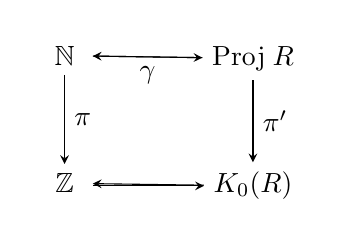
\begin{tikzpicture}
  \matrix (m) [matrix of math nodes,row sep=3em,column sep=4em,minimum width=2em]
  {
     \mathbb{N} & \proj R \\
     \mathbb{Z} & K_0(R) \\};
  \path[-stealth]
    (m-2-1.east|-m-2-2) edge node [below] {}
            node [above] {} (m-2-2)
    (m-1-2) edge node [right] {$\pi '$} (m-2-2)
    (m-1-1) edge node [below] {$\gamma$} (m-1-2)
    (m-1-1) edge node [right] {$\pi $} (m-2-1)
    (m-2-2) edge node [left] {} (m-2-1)
    (m-1-2) edge node [below] {} (m-1-1);
\end{tikzpicture}
    \end{minipage}
\end{figure}
%%%%%%%%%%%%%%%%%%%%%%%%%%%%%%%%%%%%%%%%%%%%%%%%%%%%%%%%%%

%%%%%%%%%%remark
\begin{figure}[!htb]
    \centering
    \begin{minipage}{.66\textwidth}
        \begin{obs}
Per a tot anell $R$ podem definir l'homomorfisme d'anells $\iota:\mathbb{Z}\rightarrow R$ definit per enviar $1$ a $1_R$. Tenint en compte que $\mathbb{Z}$ és un DIP i aplicant el Corol·lari \ref{RD} es dedueix $\ko (\mathbb{Z}) \cong \mathbb{Z}$. Usant la functorialitat de $\ko$ tenim que existeix una aplicació induïda $\iota_*: \mathbb{Z} \rightarrow \ko(R)$. La imatge de $\iota_*$ és el subgrup de $\ko(R)$ generat pels $R$-m.ll.f.g.
\end{obs}
    \end{minipage}%
    \begin{minipage}{0.33\textwidth}
       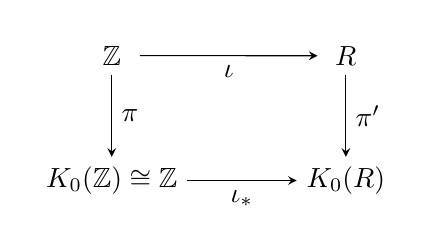
\begin{tikzpicture}
  \matrix (m) [matrix of math nodes,row sep=3em,column sep=4em,minimum width=2em]
  {
     \mathbb{Z} & R \\
     K_0(\mathbb{Z})\cong \mathbb{Z} & K_0(R) \\};
  \path[-stealth]
    (m-2-1.east|-m-2-2) edge node [below] {$\iota_*$}
            node [above] {} (m-2-2)
    (m-1-2) edge node [right] {$\pi '$} (m-2-2)
    (m-1-1) edge node [below] {$\iota$} (m-1-2)
    (m-1-1) edge node [right] {$\pi $} (m-2-1);
\end{tikzpicture}
    \end{minipage}
\end{figure}
%%%%%%%%%%%%%%%%

\begin{definition}
Donat un anell $R$ definim el \textbf{$K_0$ grup reduït} per
$$
\tilde{K}_0(R):=K_0(R)/\iota_*(\mathbb{Z})
$$
\end{definition}
En general $\tilde{K}_0(R)$ mesura la part no òbvia de $K_0(R)$, de moment hem vist que $\tilde{K}_0(R)$ desapareix si $R$ és un anell de divisió o un DIP.

\section{El cas dels anells locals}
En aquesta secció presentem el concepte d'anell local amb alguns exemples i algunes de les seves propietats fonamentals que ens permetran calcular $K_0$ per aquesta estructura algebraica.  \\

\begin{definition} 
Un anell $R$, no necessàriament commutatiu, és \textbf{local} si els elements no invertibles de $R$ formen un ideal propi bilàter $M$ de $R$.
\end{definition}

\begin{prop} \label{clocals}
Un anell $R$ és local si i només si $R$ té un únic ideal maximal per l'esquerra, i un únic ideal maximal per la dreta, i aquests coincideixen.
\end{prop}
\begin{proof}
Veiem primer $(\Rightarrow)$, si $R$ és local i $M$ és el seu ideal d'elements no invertibles, no pot existir cap ideal per l'esquerra (o dreta) propi que tingui algun element de $R\backslash M$, ja que l'ideal generat per un element invertible és tot l'anell $R$, per tant $M$ és l'únic ideal maximal per l'esquerra (o dreta). Veiem ara $(\Leftarrow)$, donat un $x\in R$, si $x$ no té inversa per l'esquerra tenim que $Rx$ és un ideal per l'esquerra propi, aquest ideal propi ha d'estar contingut en algun ideal maximal per l'esquerra, i per hipòtesi aquest ideal és únic. Similarment si $x$ no té inversa per la dreta pertany a un ideal maximal únic per la dreta. La hipòtesi de coincidència ens permet afirmar que l'ideal d'elements invertibles és bilàter.
\end{proof}

\begin{corollary}
En un anell local, si un element té inversa per un costat, és invertible.
\end{corollary}
\begin{proof}
Suposem que en un anell local existeix un element $x$ diferent de zero que té inversa per la dreta i no per l'esquerra, per una banda al tenir inversa per la dreta $x$ no pot pertànyer a cap ideal propi per la dreta. D'altra banda, com que $x$ té inversa per l'esquerra $x$ pertany a un ideal propi per l'esquerra. Usant la Proposició \ref{clocals}, tenim que $x\in M$ i $x\not \in M$.
\end{proof}


\begin{prop}\label{Zp}
Sigui $p$ un nombre primer i $k>0$, aleshores l'anell $\mathbb{Z}/(p^k \mathbb{Z})$ és local.
\end{prop}
\begin{proof}
Un ideal és en particular un subgrup, els subgrups de $\mathbb{Z}/p^k\mathbb{Z}$ són de la forma $p^{k'}\mathbb{Z}/p^k\mathbb{Z}$ amb $0\leq k' \leq k$. Per tant tots els ideals de $\mathbb{Z}/p^k\mathbb{Z}$ són principals, a més, el seu únic ideal maximal és $p\mathbb{Z}/p^k \mathbb{Z}$, usant la Proposició \ref{clocals} tenim que és un anell local.
\end{proof}

\begin{prop} \label{K[x]preLocal}
Per a tot cos $K$, i tot $p(x)\in K[x]/(x^n)$, $p(x)$ és invertible si i només si $p(0)\neq 0$. 
\end{prop}
\begin{proof}
En primer lloc observem que tots els elements de $ K[x]/(x^n)$ són de la forma
$$
a_0+a_1y+a_2y^2+\dots + a_n y^{n-1},
$$
on $y=x + (x^n)$. A més, observem que per a tot $n_1,n_2\in \mathbb{N}$, $y^{n_1}y^{n_2}=y^{n_1+n_2}$ si $n_1+n_2<n$, i en cas contrari $y=(x^n)$. Observem que en particular, $y$ és un element nilpotent, i.e. $y^n=0+(x^n)$. Feta aquesta observació, comencem la prova.
\\
Donat un $p(x)$ tal que $p(0)\neq 0$, per l'observació anterior tenim que té inversa. D'altra banda, si $p(x)$ és invertible i $p(0)=0$, existeix una expressió de la forma $$p(x)=a_1y+\dots a_{n-1}y^n,$$ per tant podem expressar $p(x)$ com a combinació lineal d'elements nilpotents, i usant el Teorema del binomi tenim que $p(x)$ és nilpotent. Tanmateix si $p(x)$ és nilpotent no pot ser invertible, provant l'altra implicació.
\end{proof}

\begin{cor} \label{K[x]local} $p(x)\in K[x]/(x^n)$ és un anell local.
\end{cor}
\begin{proof}
Per la Proposició \ref{K[x]preLocal} tenim que els element no invertibles són els que compleixen $p(0)=0$, en particular formen un ideal bilàter.
\end{proof}

\begin{definition}
Per a qualsevol anell $R$ anomenem \textbf{radical} (o radical de Jacobson) de $R$ a la intersecció dels ideals maximals per l'esquerra. Per la Proposició \ref{clocals}, en un anell local el radical coincideix amb l'ideal maximal, i.e., l'ideal format pels elements no invertibles de $R$.
\end{definition}

\begin{prop}\label{radbilater}
Per a qualsevol anell $R$ el seu radical és un ideal bilàter. 
\end{prop}
\begin{proof}
És suficient veure que $\rad R = \bigcap_{I \text{ ideal max. per l'esquerra}} \ann_R(R/I)$\footnote{$\ann_R(S)=\{r\in R | \forall s\in S, rs=0 \}$.} ja que l'anul·lador és un ideal bilàter i intersecció d'ideals bilàters és un ideal bilàter.
Per a veure ($\supset$) observem que donat un ideal maximal per l'esquerra $I$, l'anu·lador de $R/I$ clarament està contingut a $I$, per tant 
$$
\bigcap_{I \text{ ideal max. per l'esquerra}} \ann_R (R/I) \subset \bigcap_I I = \rad R
$$
Per a veure ($\subset$) usem el fet que
$$
\ann_R (R/I) = \bigcap_{\dot{x} \in R/I, \dot{x} \neq 0} \ann_R (\dot{x}),
$$
i.e., l'anul·lador de $R/I$ és intersecció d'ideals maximals per l'esquerra.
\end{proof}

\begin{obs}
Tenint en compte la prova anterior i usant que tot $R$-mòdul simple és isomorf a un quocient $R/m$ on $m$ és un ideal maximal de $R$ (es poden veure tots els detalls d'aquest resultat a [8]), tenim que $\rad R$ és el conjunt d'elements que anul·len tots els $R$-mòduls simples. A més, com que tot mòdul simple per $M_n(R)$ és isomorf a un de la forma $R^n \otimes_R M$ on $M$ és un $R$-mòduls simple, tota matriu amb entrades a $\rad R$ ha d'anul·lar tots aquests mòduls, i per tant pertany al radical de $M_n(R)$.

\end{obs}

\begin{corollary}\label{rradRdivring}
 Si $R$ és un anell local, $R/\rad R$ és un anell de divisió\footnote{$R$ és de divisió si és un anell no zero en que tot element diferent de zero és invertible, i.e., per a tot element $x\in R$ amb $x\neq 0_R$ existeix un $a\in R$ tal que $a\cdot x = x\cdot a = 1_R$}. Si $R$ és commutatiu, $R/\rad R$ és un cos.
\end{corollary}
\begin{proof}En primer lloc observem que l'anell quocient està ben definit gràcies a la Proposició \ref{radbilater}.
Usant la Proposició \ref{clocals} tenim que $\rad R$ és maximal, com que el quocient d'un anell per un ideal maximal ha de ser un anell simple, $R/\rad R$ és simple (un anell és simple si és un anell no nul que no té més ideals bilàters que el zero i ell mateix), de fet en el cas commutatiu és un cos. A més, tot element no zero ha de tenir inversa gràcies al fet que $\rad R$ en el cas dels anells locals és l'ideal format pels elements no invertibles de $R$.
\end{proof}



\begin{prop}\label{crad}
Per un anell $R$, $\rad R = \{ x\in R : \forall a \in R, 1-ax \ \text{té inversa per l'esquerra} \}$
\end{prop}
\begin{proof}
Veiem primer ($\subset$), si $x$ pertany a tot ideal maximal per l'esquerra, aleshores $Rx$ ha de pertànyer a tot ideal maximal per l'esquerra\footnote{La intersecció d'ideals per l'esquerra és un ideal per l'esquerra.}. Suposem que existeix un $a\in R$ tal que $1-ax$ no tingui inversa. Aleshores $1-ax$ ha de pertànyer a un ideal propi, i per tant en un ideal maximal per l'esquerra. Com que $ax\in M$ tenim que $1_R \in M$, que contradiu que $M$ sigui maximal \footnote{Un ideal maximal ha de ser propi.}.
Per a veure ($\supset$), suposem que per a tot $a\in R$, $1-ax$ té inversa per l'esquerra. Sigui $M$ un ideal maximal per l'esquerra, si $x\not \in M$, aleshores $Rx+M = R$. Per tant per algun $a\in R$, $1-a\in M$, fet que contradiu que $1-a$ tingui inversa per l'esquerra.
\end{proof}

\begin{prop}
Per un anell $R$ el radical coincideix amb la intersecció dels ideals maximals per la dreta.
\end{prop}
\begin{proof}
Podem definir el radical per la dreta de la següent forma:
$$
\text{r-rad} \ R = \bigcap \text{ideals max. per la dreta} = \{x\in R: \forall a\in R, 1-xa \ \text{té inversa per la dreta}\}
$$
Anem a provar que $\rad R\subset r-\rad R$, l'altre inclusió és simètrica.
Usant la Proposició \ref{radbilater} tenim que $\rad R$ és un ideal per la dreta, per tant si $x\in \rad R$, per a tot $a\in R$ tenim que $xa\in \rad R$. Aplicant la Proposició \ref{crad} sobre $xa$ i usant el fet que per a tot element $b\in R$ existeix un $c\in R$ tal que $(1-c)=b$ ($c:=1-b$) tenim que si $x\in \rad R$ i $a\in R$, existeix un $c\in R$ tal que $(1-c)(1-xa)=1$, d'aquí es dedueix $-c-xa=-cxa$, i aquesta igualtat dóna lloc a $(1-xa)(1-c)=1+xac-cxa$. Observem que $1+xac-cxa$ ha de tenir una inversa per l'esquerra, ja que $x\in \rad R$ i $xac-cxa\in \rad R$. Per tant, $(1-c)$ té una inversa per l'esquerra, a més, com que ($1-xa$) és una inversa per la dreta, i les inverses han de coincidir \footnote{El fet que les inverses coincideixin és fruit de l'associativitat de $R$, sigui $x\in R$ un element que té $y\in R$ per inversa per l'esquerra i $z\in R$ per inversa per la dreta, per una banda tenim $(yx)z = z$, d'altra banda $y(xz)=y$, per tant $y=z$, i.e., la inversa per la dreta coincideix amb la inversa per l'esquerra. }, $1-xa$ també és inversa per l'esquerra, i per tant $1-xa$ és invertible amb inversa $1-c$. Així doncs $\rad R \subset \text{r-rad}\ R$. 
\end{proof}

\begin{theorem}[Lema de Nakyama]
Suposem que $R$ és un anell i $M$ és un $R$-m.f.g tal que $(\rad R)M=M$. Aleshores $M=0$.
\end{theorem}

\begin{proof}
Si $M\neq 0$, considerem un conjunt de generadors $x_1,\dots ,x_m \in M$ amb $m$ tan petit com sigui possible. Observem que per construcció s'ha de complir $x_j\neq 0$, ja que si existís algun $x_j=0$, $m$ no seria tan petita com seria possible. Per hipòtesi tenim que $(\rad R) M = M$, usant aquesta hipòtesi i el conjunt generador $x_1,\dots , x_m$, tenim que existeixen $r_1, \dots ,r_m \in \rad R$, tal que $x_m=r_1x_1 + \dots + r_m x_m$. D'aquí es dedueix $$(1-r_m)x_m=r_1x_1+\dots + r_{m-1}x_{m-1}.$$
Usant la Proposició \ref{crad} tenim que $(1-r_m)$ és invertible i en conseqüència podem expressar $x_m$ com a combinació lineal de $x_1,\dots , x_{m-1}$, i per tant $m$ no és mínim, contradicció.
\end{proof}

\begin{corollary}\label{cNakayamas} Si $R$ és un anell, $M$ un $R$-m.f.g. i $x_1,\dots x_m \in M$, aleshores $x_1,\dots,x_m$ generen $M$ si i només si les imatges $\dot{x}_1\dots \dot{x}_m$ generen $M/(\rad R) M$ com a $R/\rad R$-mòdul.
\end{corollary}
\begin{proof}
Si $x_1,\dots ,x_m$ generen $M$ és trivial veure que $\dot{x}_1,\dots,\dot{x}_m$ generen $M/\rad (R)M$.
Veiem la implicació no trivial, sigui $N=M/(\sum_i Rx_i)$, tenim que $$N/\rad(R)N=M/(\rad R M + (\sum_i Rx_i))=M/M=0,$$ per tant $\rad(R)N=N$. Aplicant ara la proposició anterior tenim que $N=0$, i en conseqüència $M=(\sum_i Rx_i)$.

\end{proof}

\begin{theorem}
Si $R$ és un anell local, no necessàriament commutatiu, aleshores tot $R$-m.p.f.g. és lliure amb un rang unívocament determinat. En particular $K_0(R) \cong \mathbb{Z}$ i té per element generador la classe de mòduls de rang 1.
\end{theorem}
\begin{proof}
Pel Corol·lari \ref{rradRdivring} tenim que $D:=R/\rad R$ és un anell de divisió, recorda que tot anell de divisió és un DIP. Si $M$ és un $R$-m.p.f.g podem assumir $M\oplus N=R^k$ per algun $k$. Aleshores $M/(\rad R) M$ i $N/(\rad R)N$ són $D$-mòduls, usant el Teorema \ref{defRangDIP} tenim que són lliures. Si denotem per $m$ i $n$ als seus respectius rangs cal que es compleixi $m+n=k$. Així doncs podem triar elements bàsics d'aquests mòduls i tiar-los enrere de forma que tinguem $x_1,\dots , x_m\in M$ i $x_{m+1}, \dots , x_k \in N$. Pel Corol·lari \ref{cNakayamas}, aquests elements generen $R^k$. Falta veure que $x_1, \dots ,x_k$ són una base de $R^k$. Això mostrarà en particular que $x_1, \dots, x_m$ són un conjunt generador de $M$ linealment independent, per tant $M$ és lliure amb un rang inequívocament determinat
$$
\rank M  = \dim_D M / (\rad R)M.
$$
\indent Sigui $e_1,\dots , e_k$ una base estàndard de $R^k$. Com que tenim dos conjunts generadors de $R^k$, cada conjunt generador pot ser expressat en termes de l'altre, i.e., existeixen elements $a_{ij}, b_{ij}\in R$ amb 
$$
e_i = \sum_{j=1}^k a_{ij}x_j, \  x_i = \sum_{j=1}^k b_{ij}e_j
$$
Per tant tenim
$$
e_i = \sum_{j=1}^k a_{ij} \sum_{l=1}^k b_{jl}e_l,
$$
i conseqüentment
$$
\sum_{j=1}^{k} \sum_{l=1}^k (a_{ij}b_{jl}-\delta_{il})e_l=0,
$$
i si $A=(a_{ij})$, $B=(b_{ij})$, significa que , com que els $e_l$ són linealment independents, $AB=I$. Amb una substitució simètrica tenim
$$
\sum_{j=1}^{k} \sum_{l=1}^k (b_{ij}a_{jl}-\delta_{il})x_l=0,
$$
i com que els $x_l$ són linealment independents mòdul el radical de $R$, usant l'observació que precedeix la Proposició \ref{radbilater} tenim que $BA-I \in M_n (\rad R) \subset \rad M_n(R)$. Per la proposició \ref{crad}, $BA$ és invertible, per tant $B$ és invertible. Com que $A$ era inversa per l'esquerra de $B$, això mostra que també és inversa per la dreta, i.e., $BA=I$. Provant que $x_1,\dots,x_m$ és una base de $R^k$
\end{proof}
%%%%%%%%%%%%%%%%%%%%%%%%%%%%%%%%%%%%%

\section{El grup $K_0$ relatiu i el Teorema d'Excisió}
El primer objectiu d'aquesta secció és definir el grup relatiu $K_0(R,I)$ i trobar la successió exacta que relaciona $K_0(R)$ amb $K_0(R/I)$, aquesta successió l'extendrem en el següent capítol i ens permetrà calcular $K$-grups. El segon objectiu d'aquesta secció és provar un anàleg de l'axioma de l'excisió de teoria de la homologia, de fet durant aquesta secció es pot veure que hi ha cert paral·lelisme entre la teoria de la homologia i $K$-teoria algebraica; aquest anàleg ens permetrà definir $K_0(I)$ on $I$ és un anell sense necessitat de tenir element unitat, i veurem la relació entre $K_0(I)$ i el $K_0$ relatiu. \\ \\
\indent  Per a trobar una successió exacta que relacioni $K_0(R/I)$ i $K_0(R)$ necessitem saber que és una successió exacta.
\begin{definition}
Diem que una successió de grups i homomorfismes de grups 
$$
G_0 \xrightarrow{f_1} G_1 \xrightarrow{f_2} G_2 \xrightarrow{f_3} \dots \xrightarrow{f_n} G_n
$$
és \textbf{exacta} si la imatge de cada homomorfisme és igual al nucli del següent, i.e., $\im (f_k) = \ker (f_{k+1})$. Aquesta successió d'homomorfismes i grups pot ser finita o infinita.  En particular ens interessen les successions \textbf{exactes  i curtes}, que són successions de la forma:
$$
0 \rightarrow A \xrightarrow{f} B \xrightarrow{g} C \rightarrow 0,
$$
una successió exacta curta ha de complir que $f$ sigui un \textit{monomorfisme}\footnote{Un monomorfisme és un homomorfisme injectiu.} i $g$ un \textit{epimorfisme}\footnote{Els epimorfismes és un homomorfisme exhaustiu.}. Una successió exacta és \textbf{escindida} si és curta i existeix un homomorfisme $h: C\rightarrow B$ tal que $g\circ h$ sigui la identitat sobre $C$.
\end{definition}
Introduïm ara els conceptes necessaris per definir $K_0(R/I)$.
\begin{definition}
Sigui $R$ un anell i $I\subset R$ un ideal (en aquesta secció els ideals sempre seran bilàters). El \textbf{doble d'un anell} $R$ sobre $I$ és el subanell del producte cartesià $R\times R$ donat per
$$
D(R,I) = \{ (x,y)\in R\times R: x-y\in I \}
$$


\end{definition}

\begin{obs}
Si $p_1: D(R,I) \rightarrow R$ és la projecció a la primera coordenada, podem identificar $I$ com a $\ker p_1$, per tant existeix una successió exacta curta
$$
0 \rightarrow I \rightarrow D(R,I) \xrightarrow{p_1} R\rightarrow 0,
$$
a més si definim $h: R \rightarrow R\times R$ a l'assignació diagonal $x\mapsto (x,x)$, tenim que $p_1 \circ h$ és la identitat a $C$, i per tant la successió exacta escindeix.

\end{obs}

\begin{definition} \label{K0relatiu}
El grup \textbf{$K_0$-relatiu} d'un anell $R$ i un ideal $I$ ve definit per 
$$
K_0(R,I) = \ker ((p_1)_*): K_0(D(R,I)) \rightarrow K_0(R)).
$$
\end{definition}

Un fenomen íntimament relacionat amb l' estudi de K-teoria relativa és el fet que tota matriu sobre $R/I$ pot ser pujada a una matriu sobre $R$; tanmateix una matriu invertible no sempre pot ser pujada a una matriu invertible. 
 
\begin{lema} \label{InvAsc} \label{matrixlifting}
Sigui $R$ un anell i $I\subset R$ un ideal.\\Aleshores si $A\in GL(n,R/I)$,    $\left( \begin{matrix}
  A & 0 \\
  0 & A^{-1}
 \end{matrix} \right) \in GL(2n,R/I)$ puja a una matriu $GL(2n,R)$.
\end{lema}


\begin{proof}
En primer lloc, observem que es compleix
\begin{equation}
\left( \begin{matrix}
  A & 0 \\
  0 & A^{-1}
 \end{matrix} \right)
 =
 \left( \begin{matrix}
  1 & A \\
  0 & 1
 \end{matrix} \right)
 \left( \begin{matrix}
  1 & 0 \\
  -A^{-1} & 1
 \end{matrix} \right)
\left( \begin{matrix}
  1 & A \\
  0 & 1
 \end{matrix} \right)
\left( \begin{matrix}
  0 & -1 \\
  1 & 0
 \end{matrix} \right) 
\end{equation}
La prova consisteix a constatar que cada matriu del producte de la factorització anterior puja a una matriu invertible. En concret la matriu $\left( \begin{matrix}
  0 & -1 \\
  1 & 0
 \end{matrix} \right) $ clarament puja a una matriu invertible. Siguin $B,C\in M_n(R)$ les preimatges de les matrius $A$ i $A^{-1}$ respectivament; $B$ i $C$ no són necessàriament invertibles, però les matrius 

 $$\left( \begin{matrix}
  1 & B \\
  0 & 1
 \end{matrix} \right) 
  i 
\left( \begin{matrix}
  1 & 0 \\
  -C & 1
 \end{matrix} \right) 
 $$
 sí que ho són.

\end{proof}

\begin{theorem}\label{K0relatiuT}
Sigui $R$ un anell i $I\subset R$ un ideal. Aleshores existeix una successió exacta curta
$$
K_0(R,I) \rightarrow K_0(R) \xrightarrow{q_*} K_0(R/I)
$$
on $q_*$ és induïda per l'aplicació quocient $q:R\rightarrow R/I$ i l'aplicació $K_0(R,I) \rightarrow K_0(R)$ és induïda per $p_2: D(R,I)\rightarrow R$ (la projecció a la segona component).
\end{theorem}

\begin{proof}
Per simplicitat si $A$ és un element de $R$ o una matriu amb entrades a $R$, sovint denotarem $q(A)$, la matriu corresponent amb entrades sobre $R/I$, per $\dot{A}$. \\
En primer lloc volem veure que la imatge de la primera aplicació està continguda en el nucli de la segona. Sigui $[e]-[f]\in K_0(R,I)$, on $e=(e_1,e_2)$, $f=(f_1,f_2)\in \idem (D(R,I)).$ 
Usant el Corol·lari \ref{K0Cartesian} tenim que $K_0(R\times R)\cong K_0(R)\times K_0(R)$, aleshores la imatge de $[e]-[f]$ és $([e_1]-[f_1],[e_2]-[f_2])$, per tant
$$
q_* \circ(p_2)_* ([e]-[f]) = q_* ([e_2]-[f_2])=[\dot{e}_2]-[\dot{f}_2],$$
mentre que $[e_1]-[f_1]=0$, ja que per hipòtesi $[e]-[f]\in \ker(p_1)_*$. Però com que $e,f\in \idem D(R,I)$, $\dot{e_1}=\dot{e_2}$ i $\dot{f_1}=\dot{f_2}$. Per tant
$$
[\dot{e_2}]-[\dot{f_2}] =  [\dot{e_1}]-[\dot{f_1}] = q_*([e_1]-[f_1])=0
$$
Per tant la imatge de la primera aplicació està continguda al nucli de la segona. Veiem ara el recíproc; siguin $e,f\in \idem (R)$ dels que $q_*([e]-[f])=0$. Aleshores existeix un $r$ prou gran tal que
$$
\dot{e} \oplus \dot{1}_r = q(e\oplus 1_r) \sim \dot{f} \oplus \dot{1}_r = q(f \oplus 1_r)
$$
a $GL(R/I)$. Canviant $e$ per $e \oplus 1_r$ i $f$ per $f \oplus 1_r$, podem assumir que $\dot{f}$ i $\dot{g}$ són conjugades, i.e., existeix una matriu $\dot{g}\in GL(R)$ tal que $\dot{f} = \dot{g} \dot{e} (g)^{-1}$. Observem que la matriu $\dot{g} \oplus (\dot{g})^{-1}$ conjuga $\dot{e}\oplus \dot{0}$ a $\dot{f}\oplus \dot{0}$, i usant el Lema \ref{matrixlifting} puja a una matriu $h\in GL(R)$. Per tant podem canviar $f$ per $f\oplus 0$ i $e$ per $h(e\oplus 0)h^{-1}$ sense canviar $[e]$ i $[f$], i reduir-nos al cas en que $\dot{e}=\dot{f}$. Així doncs $(e,f)\in \idem (D(R,I))$. Aleshores la imatge de la classe $[(e,e)]-[(e,f)]\in K_0(D(R,I)$ és $0$ per $(p_1)*$ i $[e]-[f]$ per $(p_2)_*$.
\end{proof}

Ara veurem que té sentit definir $K_0$ sobre un anell sense unitat, a més veurem que el grup relatiu $K_0(R,I)$ és isomorf a $K_0(I)$, on $I$ és un anell sense unitat.

\begin{definition}
Sigui $I$ un anell que no tingui necessàriament element unitat. Anomenem \textbf{anell obtingut al afegir un element unitat a $I$} a el grup abelià $I \oplus \mathbb{Z}$ amb el producte definit per 
$$
(x,n)\cdot (y,m) = (xy+ny+mx, mn),
$$
$x,y \in I;$ $m,n\in \mathbb{Z}$. Aquest anell el denotarem $I_+$. Notem que l'element $(0,1)\in I_+$ és el seu element unitat.
\end{definition}

\begin{obs}

Si $\alpha :  I \rightarrow I'$ és un homomorfisme de la categoria d'anells sense unitat, llavors $\alpha$ estén a un únic homomorfisme d'anells amb unitat $I_+ \xrightarrow{\alpha_+}I'_+$. 
Observem que en el cas que $I$ tingui element unitat, existeix un isomorfisme unitari\footnote{Una aplicació es unitària si envia la imatge de l'element unitat és element unitat. En aquest cas $\alpha (0,1) = (e,1)$.} $\alpha: I_+ \rightarrow I \times \mathbb{Z}$ definit per
$$
\alpha (x,n) = (x+ne, n),
$$
ja que 

\begin{align*} 
\alpha((x,n)\cdot (y,m)) &= \alpha(xy+ny+mx, mn) \\
&=(xy+ny+mx+mne,mn)\\
&=(x+ne,n) \cdot (y+me, m) \\
&=\alpha (x,n) \cdot \alpha (y,m)
\end{align*}

\end{obs}


\begin{definition}
Sigui $I$ un anell el que no tingui necessàriament element unitat. Llavors existeix una successió exacta curta escindida
\begin{equation} \label{suc}
0 \rightarrow I \rightarrow I_+ \xrightarrow{\rho} \mathbb{Z} \rightarrow 0.
\end{equation}
on $\rho$ està definida per $\rho(x,n)=n$. En aquest context definim
$$
K_0(I):=\ker (\rho_*: K_0(I_+)\rightarrow K_0(\mathbb{Z})\cong \mathbb{Z}).
$$
Pot semblar que la definició és ambigua, ja que si $I$ té unitat hem donat dues definicions diferents de $K_0(I)$. En aquest cas veiem que les definicions són coincidents, ja que si $I$ té unitat. $$I_+ \cong I \times \mathbb{Z},$$ i usant l'observació anterior $K_0(I_+) \cong K_0(I) \oplus K_0(\mathbb{Z})$, i $\ker \rho_*$ només està format per elements del primer sumand. Per tant la nova definició coincideix amb l'anterior.
\end{definition}


\begin{theorem}[Escisió]
Si $I$ és un ideal bilàter en un anell $R$, aleshores $K(R,I)\cong K_0(I)$ (i per tant no depèn de $R$, només en l'estructura de $I$ com a anell sense unitat).
\end{theorem}



 
 
 
 \begin{figure}[!htb]
    \centering
    \begin{minipage}{.66\textwidth}
\begin{proof}\renewcommand{\qedsymbol}{}         
         Definim l'homomorfisme unitari \\$\gamma: I_+ \rightarrow D(R,I)$ per
 $$
 (x,n) \mapsto (n \cdot 1, n\cdot 1 + x),$$ amb   $x\in I$,  $n \in \mathbb{Z}$, observem que el diagrama commuta. \\Per tant $\gamma_*: K_0(I_+) \rightarrow K_0(D(R,I))$ envia $\ker \rho_*$ a $\ker (p_1)_*$, i.e., envia $K_0(I)$ a $K_0(R,I)$.
 \end{proof}
    \end{minipage}%
    \begin{minipage}{0.33\textwidth}
            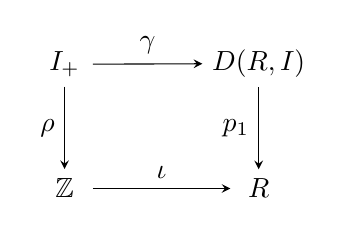
\begin{tikzpicture}
  \matrix (m) [matrix of math nodes,row sep=3em,column sep=4em,minimum width=2em]
  {
     I_+ & D(R,I) \\
     \mathbb{Z} & R \\};
  \path[-stealth]
    (m-2-1.east|-m-2-2) edge node [below] {}
            node [above] {$\iota$} (m-2-2)
    (m-1-2) edge node [left] {$p_1$} (m-2-2)
    (m-1-1) edge node [above] {$\gamma$} (m-1-2)
    (m-1-1) edge node [left] {$\rho $} (m-2-1);
\end{tikzpicture}
    \end{minipage}
\end{figure}
\begin{proof}[]
\indent Per a veure que l'aplicació és exhaustiva considerem una classe classe $[e]-[f]\in K_0(R,I)$, on $e=(e_1,e_2)$, $f=(f_1,f_2)\in \idem (D(R,I))$ i $[e_1]=[f_1]$ a $K_0(R)$.
 A partir de canviar $e$ i $f$ per $e\oplus 1_r$ i $f\oplus 1_r$ respectivament per a una $r$ prou gran, podem assumir que $e_1$ i $f_1$ són conjugats a $GL(R)$, i.e., existeix una matriu invertible $g$ tal que $e_1=gf_1g^{-1}$. Així doncs si canviem $(f_1,f_2)$ per $(gf_1g^{-1}, gf_2g^{-1})$ podem assumir que $f_1=e_1$.  D'altra banda si $e$ és una matriu $s\times s$, podem canviar $e$ i $f$ per $e\oplus (1_s-e_1,1_s-e_1)$ i $f\oplus (1_s-e_1,1_s-e_1)$ respectivament, obsevem que hi ha una matriu invertible $h$ de mida $2s\times 2s$ amb entrades a $R$ que conjuga $e_1\oplus (1_s-e_1)$ i $1_s\oplus 0_s$. Conjugant-ho tot per $h$ ens reduim en el cas on $e=(1_s\oplus 0_s, e_2)$, $f=(1_s \oplus 0_s, f_2)$, a més, com que $e$ i $f$ són matrius sobre $D(R,I)$, $e_2-(1_s \oplus 0_s)$ i $f_2-(1_s\oplus 0_s)$ tenen entrades a $I$. Així doncs observem que $[e]-[f]$ és la imatge de $K_0(I)$.
\\ \indent Faflta veure que $\gamma_*$ és injectiva, tot element de $K_0(I)$ pot ser expresat com $[e]-[f]$, on $e,f\in \text{Idem}(I_+)$ i $\text{rank} \ \rho(e) = \text{rank} \ \rho (f)$. De la mateixa forma que a la prova de l'exhaustivitat, a partir de prendre suma directa amb $1_r-f$ i conjugar podrem assumir que $f=1_r$, $\text{rank} \ \rho (e)=r$. A més podem assumir que $g\rho (e) g^{-1}=1_r$ per algún $g\in GL(\mathbb{Z})$. Considerant $g$ com un element de $GL(I_+)$ via la successió exacta escindida (\ref{suc}) podem reemplaçar $e$ per $geg^{-1}$ i assumir que $\rho(e)=1_r$. Ara si $\gamma_*([e]-[1_r])=0$ significa que 
$$
[(1_r,e)]=[(1_r,1_r)] \ \text{a} \ K_0(D(R,I)).
$$
Si és necessari podem estabilitzar a través d'augmentar $r$ i assumir que existeix una matiru $(g_1,g_2)\in GL(D(R,I))$ amb 
$$
g_11_rg_1^{-1}=1_r, \ g_2e_2g_2^{-1}=1_r.
$$
Aleshores $(1, g_1^{-1}g_2) \in GL(D(R,I))$ i 
$$
(
(g_1^{-1}g_2)e(g_1^{-1}g_2)^{-1} = g_1^{-1}(g_2eg_2^{-1})g_1 = g_1^{-1}1_rg_1 = 1_r.
$$
Com que $g_1^{-1}g_2 \cong 1 \mod I$, $g_1^{-1}g_2$ pertany a $GL(I_+)$ i això significa que $[e]-[1_r]=0$ a $K_0(I)$, i per tant el nucli $\gamma_*$ és trivial.
\end{proof}

 

% Chapter 1

\chapter{Construcció del Grup $K_1$} % Main chapter title

\label{Chapter3} % For referencing the chapter elsewhere, use \ref{Chapter1} 

En àlgebra lineal es comença estudiant espais vectorials i la seva dimensió, i es procedeix amb l'estudi de les transformacions lineals i els seus invariants, com el determinant, les formes canòniques... \\
Similarment en $K$-teoria algebraica comencem estudiant  mòduls projectius i la seva classificació a $K_0$, i continuem estudiant la classificació d'automorfismes de mòduls lliures i projectius, i.e., invariants de matrius invertibles. \\
Així doncs, la relació entre $K_0$ i $K_1$ és la mateixa que hi ha entre transformacions lineals invertibles i els espais vectorials. \\
\indent De la mateixa forma que un homomorfisme $K_0(R)\rightarrow G$ correspon a la generalització del concepte de rang, un homomorfisme de grups $K_1(R)\rightarrow G$ correspon a generalitzar el determinant de matrius invertibles sobre $R$. \\
\indent L'objectiu d'aquest capítol és definir el grup $K_1$ a partir de matrius sobre un anell $R$ i obtenir alguns resultats que ens facilitin el càlcul del grup $K_0(R)$, la construcció exposada segueix en gran part [1], també presentem resultats i observacions interessants de [2] i la resolució de part dels problemes plantejats a [1], com el càlcul de $K_1$ per a $\mathbb{Z}/(m)$, $K[x]$ i $\mathbb{H}$.\\
A la secció on estudiem el cas dels quaternions, cal mencionar que per a la introducció a l'anell dels quaternions hem usat [3], també hem usat [4] i [5] per a introduir el determinant de Dieudonné. \\
\indent Començarem per definir $K_1$ a través de matrius invertibles sobre un anell $R$, estudiarem el cas d'un cos i intentarem generalitzar el mateix resultat per a anells de divisió, anells locals i dominis euclidians. També calculem $K_1$ d'alguns anells interessants, en particular hem dedicat una secció al càlcul de $K_1(\mathbb{H})$, ja que no només uso els resultats de les seccions anteriors, sinó que també presento el determinant de Dieudonné per al càlcul de $K_1(R)$. Finalment definirem el grup relatiu $K_1(R,I)$ que ens permetrà formular una successió exacta que relaciona $K_0$ i $K_1$ proveint-nos de més eines per al càlcul de $K$-grups.

\section{Definició de $K_1$}
\begin{definition}
Sigui $R$ un anell (amb unitat), anomenarem \textbf{matriu elemental}, i la denotem per $e_{ij}(a)$, a la matriu $n\times n$ formada per $1_R$'s a la diagonal, $a\in R$ a la posició $(i,j)$, on $i\neq j, 1\leq i,$ $j\leq n$, i $0_R$'s a la resta d'entrades.
\end{definition}

\begin{obs}
Les matrius elementals són invertibles, en concret $e_{ij}(a)^{-1}=e_{ij}(-a)$, per tant són elements de $GL(n,R)$, i a més generen un subgrup que denotarem $E(n,R)$. A partir de la incrustació usual de $GL(n,R)$ a $GL(n+1,R)$ presentada a la Definició \ref{incrustacio}, podem incrustar $E(n,R)$ a $E(n+1,R)$. La unió finita dels $E(n,R)$ és denotada per $E(R)$ i usualment s'anomena \textbf{grup de matrius elementals}.\footnote{Observem que el grup de matrius elementals és un abús de notació. Ens permetem aquest abús de notació, entenent que el grup de matrius elementals és la unió finita de tants $E(n,R)$ com ens convingui.}
\end{obs}

\begin{obs}
Tota matriu elemental es pot expressar com $e_{ij}(r) = I_n + r\epsilon_{ij}$, on $\epsilon_{ij}$ és la matriu amb $1_R$ a la posició $(i,j)$ i zeros a la resta. Observem que el producte compleix
$$
\epsilon_{ij}\epsilon_{kl} =
\begin{cases}
0 \ \text{si} \ j\neq k \\
\epsilon_{il} \ \text{si} \ j=k.
\end{cases}
$$

Usant les matrius elementals podem causar una de les tres transformacions elementals usades en el mètode de reducció de Gauss, en concret

\begin{equation*}
e_{ij}(r)(A) = (I+r\epsilon_{ij}) \sum_{k,l} a_{kl} \epsilon_{kl} = \sum_{k,l}a_{kl}\epsilon_{kl} + \sum_l ra_{jl}\epsilon_{il}
=
\sum_{k\neq i} \sum_{l}a_{kl}\epsilon_{kl} + \sum_{l}(a_{il}+ra_{jl})\epsilon_{il}
\end{equation*}
\textit{i.e.}, multiplicar $e_{ij}(r)$ per l'esquerra de $A$ equival a sumar $r$ vegades la fila $j$ a la fila $i$ de la matriu $A$.  Les altres dues transformacions elementals usades en el mètode de Gauss també es poden expressar com a producte de matrius, en concret multiplicar $P_{i,j}$ per l'esquerra d'$A$ 
$$
P_{i,j}=I_n - \epsilon_{ii} - \epsilon_{jj} + \epsilon_{ij} + \epsilon_{ji}
$$
canvia de posició les files $i$ i $j$ de la matriu $A$, i finalment si $u\in R^{x}$, el producte de $d_i(u)$ per l'esquera de $A$ multiplica la fila $i$-èssima d'$A$ per $u$.
$$
d_i(u)=I_n+(u-1)\epsilon_{ii}
$$
Així doncs, les tres transformacions usades en el mètode de Gauss es poden expressar com a producte de matrius invertibles, però només una d'aquestes tres pertany a $E(R)$, a més, només la primera deixa el determinant invariant, per aquest motiu $E(R)$ està íntimament relacionat amb $K_1(R)$. 
\end{obs}

\begin{lemma} \label{triangular}
Les matrius triangulars superiors (i triangulars inferiors) sobre un anell $R$ amb 1's a la diagonal pertanyen a $E(R)$.
\end{lemma}

\begin{proof}
Sigui $A=(a_{i,j}) \in GL(n,R)$ una matriu triangular superior amb zeros a la diagonal, aleshores
$$
A'=(a'_{i,j})=A_{12}(-a_{12})e_{23}(-a_{23})\dots e_{n-1,n}(-a_{n-1,n})
$$
és una matriu triangular superior amb 1's a la diagonal i zeros a la diagonal secundària superior. Similarment
$$
A''=(a''_{i,j})=A'e_{13}(-a'_{13})e_{24}(-a'_{24})\dots e_{n-2,n}(-a'_{n-2,n})
$$
és triangular superior amb 1's a la diagonal i zeros a la primera i segona diagonals secundàries superiors. Continuant el procés per inducció construïm una successió
$$
A, \ A', \ A'', \dots , \  A^{(n-1)}
$$
de matrius a $GL(n,R)$, on per construcció la matriu $A^{(k)}$ és una matriu $(n\times n)$ triangular superior amb 1's a la diagonal i zeros a $a_{ij}^{(k)}$ amb $0<j-i\leq k$. En particular $A^{(n-1)}$ és la matriu identitat $n\times n$, a més cada matriu de la successió s'obté multiplicant la matriu anterior per una matriu de $E(n,R)$. Per tant existeix una matriu $B\in E(n,R)$ tal que $$A=A^{(n-1)}B=B \in E(n,R),$$ tal com volíem. Un raonament similar es pot usar per al cas diagonal inferior.
\end{proof}

\begin{cor} \label{matriuElemental}
Sigui $A\in GL(n,R)$, la matriu $2n\times 2n$ 
$\left( \begin{matrix}
  A & 0 \\
  0 & A^{-1}
 \end{matrix} \right)$ 
 pertany a $E(2n,R)$.
\end{cor}

\begin{proof}
Recordant la prova del Lema \ref{InvAsc} tenim 
\begin{equation}
\left( \begin{matrix}
  A & 0 \\
  0 & A^{-1}
 \end{matrix} \right)
 =
 \left( \begin{matrix}
  1 & A \\
  0 & 1
 \end{matrix} \right)
 \left( \begin{matrix}
  1 & 0 \\
  -A^{-1} & 1
 \end{matrix} \right)
\left( \begin{matrix}
  1 & A \\
  0 & 1
 \end{matrix} \right)
\left( \begin{matrix}
  0 & -1 \\
  1 & 0
 \end{matrix} \right) 
\end{equation}
aplicant el Lema \ref{triangular} tenim que les primeres tres matrius del costat dret de la igualtat anterior pertanyen a $E(2n,R)$. Per a veure que la darrera matriu també hi pertany, veiem que ve generada per matrius elementals:
$$
 \left( \begin{matrix}
  0 & -1 \\
  1 & 0
 \end{matrix} \right)
 =
 \left( \begin{matrix}
  1 & -1 \\
  0 & 1
 \end{matrix} \right)
\left( \begin{matrix}
  1 & 0 \\
  1 & 1
 \end{matrix} \right)
\left( \begin{matrix}
  1 & -1 \\
  0 & 1
 \end{matrix} \right) .
$$
\end{proof}


\begin{definition}
Siguin $x$ i $y$ dos elements d'un grup $G$, definim el \textbf{commutador de la parella d'elements} com $[x,y]:=xyx^{-1}y^{-1}$. Observem que $[x,y]^{-1}=[y,x]$, i per tant, el producte finit de commutadors $[x,y]$ amb $x,y \in G$ formen un subgrup de $G$, el denotem per $[G,G]$ i s'anomena \textbf{subgrup commutador} de $G$. A més es compleix $z[x,y]z^{-1}=[zxz^{-1},zyz^{-1}]$ i per tant $[G,G]$ és un subgrup normal de $G$. Usant aquest fet podem definir el quocient 
$$
G_{\text{ab}} = G/[G,G],
$$
que s'anomena grup abelianitzat de $G$.
\end{definition}

\begin{prop}
Donat un grup $G$, el grup abelianitzat $G_\text{ab}$ és abelià, de fet, és el quocient abelià maximal de $G$, \textit{i.e.}, si $H\vartriangleleft G$ i $G/H$ és abelià aleshores $H$ conté $[G,G]$. \footnote{De fet, el recíproc també és cert, [2] Proposició 9.2.}

\end{prop}
\begin{proof}
La commutativitat del grup és deguda a 
$$
[x[G,G], y[G,G]] = [x,y][G,G] = [G,G].
$$
D'altra banda si $H\vartriangleleft G$ i $G/H$ és abelià, aleshores per a tot $x,y\in G$, $[x,y]H=[xH,yH]=H$ a $G/H$. Per tant $[G,G]\subseteq H$.
\end{proof}

\begin{obs}
Les matrius elementals sobre un anell $R$ compleixen la propietat 
\begin{eqnarray}
e_{ik}(a)e_{kj}(b)e_{ik}(a)^{-1}e_{kj}(b)^{-1}&=&e_{ij}(ab),  \label{prodMatriusConvenient}
\end{eqnarray}
per a $i,j,k$ diferents entre si.
\end{obs}

\begin{prop}[Lema de Whitehead]
Sigui $R$ un anell, 
$$[GL(R),GL(R)] = [E(R),E(R)] = E(R).$$
\end{prop}

\begin{proof}
En primer lloc observem que usant l'observació anterior tenim 
$$
e_{ij}(a)=[e_{ik}(a),e_{kj}(1)]
$$
per $i,j$ i $k$ diferents, i.e., cada generador de $E(R)$ és el commutador de dos elements generadors, per tant $[E(R),E(R)]=E(R)$ . \\ \indent D'altra banda, com que $E(R)\subseteq GL(R)$, $[E(R),E(R)] \subseteq [GL(R), GL(R)]$. Veiem ara el recíproc, siguin $A,  B \in GL(n,R)$. Podem incrustar $GL(n,R)$ a $GL(2n,R)$ i calcular
$$
\left( \begin{matrix}
  ABA^{-1}B^{-1} & 0 \\
  0 & 1
 \end{matrix} \right) =  
 \left( \begin{matrix}
  AB & 0 \\
  0 & B^{-1}A^{-1}
 \end{matrix} \right)
 %
 \left( \begin{matrix}
  A^{-1} & 0 \\
  0 & A
 \end{matrix} \right)
%
 \left( \begin{matrix}
  B^{-1} & 0 \\
  0 & B
 \end{matrix} \right) 
 $$
Usant el Corol·lari \ref{matriuElemental}, totes les matrius del costat dret de la igualtat pertanyen a $E(2n,R)$, per tant 
$$ABA^{-1}B^{-1}\in E(R)$$
\end{proof}

\begin{definition}
Sigui $R$ un anell amb unitat, denotarem per $K_1(R)$ el \textbf{grup abelianitzat} $GL(R)_\text{ab}=GL(R)/E(R)$. 
\end{definition}

\begin{obs}
Si $\varphi : R\rightarrow S$ és un homomorfisme d'anells $\varphi : R\rightarrow S$, indueix una aplicació al grup de matrius invertibles de $GL(R)$ a $GL(S)$, i aquest indueix un homomorfisme de $K_1(R)$ a $K_1(S)$. Per tant $R\rightsquigarrow K_1(R)$ és un functor entre la categoria d'anells a la de grups abelians.
\end{obs}

Podem identificar $K_1(R)$ com el grup de les formes canòniques, sota les transformacions elementals per files i columnes, de matrius invertibles sobre $R$. En particular, si $K_1(R)$ és trivial significa que tota matriu invertible pot ser reduïda per files i columnes a la matriu identitat.

\begin{obs}
Donades dues matrius invertibles sobre un anell $A,B\in GL(R)$, podem expressar el producte de les classes $[A],[B]\in R$ de la forma intuïtiva $[A]\cdot [B] = [AB]$, tanmateix aquest producte també es pot expressar com 
$A\oplus B =
 \left( \begin{matrix}
  A & 0 \\
  0 & B
 \end{matrix} \right)
$
ja que aplicant el Corol·lari \ref{matriuElemental} sobre la igualtat
$$
\left( \begin{matrix}
  A & 0 \\
  0 & B
 \end{matrix} \right) =  
 \left( \begin{matrix}
  AB & 0 \\
  0 & 1
 \end{matrix} \right)
 %
 \left( \begin{matrix}
  B^{-1} & 0 \\
  0 & B
 \end{matrix} \right)
 $$
dóna lloc a la igualtat
$$
[A\oplus B] = [AB\oplus 1] = [AB]
$$
 \end{obs}

\begin{prop} \label{K1Cartesian}
Siguin $R_1$ i $R_2$ anells, aleshores 
$$
K_1(R)\cong K_1(R_1) \times K_2(R_2).
$$
\end{prop}
\begin{proof}
Observem que existeix un isomorfisme $GL(R_1\times R_2) \cong GL(R) \times GL(R_2)$ definit per $$((a_{ij},b_{ij})) \mapsto ((a_{ij}),(b_{ij})).$$ Aleshores
$$
e_{ij}((r,s)) \mapsto (e_{ij}(r_1),  e_{ij}(r_2)),
$$
i per tant l'isomorfisme envia $E(R_1\times R_2)$ a $E(R_1)\times E(R_2)$; a més $(e_{ij}(r_1),  e_{ij}(r_2))$ generen $E(R_1)\times E(R_2)$ i per tant hi ha un isomorfisme induït
$$
K_1(R_1\times R_2) \cong \frac{GL(R_1)\times GL(R_2)}{E(R_1)\times E(R_2)} \cong K_1(R_1) \times K_1(R_2)
$$
definit per 
$$
(a_{ij},b_{ij}) E(R_1\times R_2) \mapsto ((a_{ij})E(R_1), (b_{ij})E(R_2)).
$$

\end{proof}

\begin{prop}[Invariància de Morita sobre $K_1$] Per a tot anell $R$
$$
K_1(R)\cong K_1(M_n(R)).
$$
\end{prop}
\begin{proof}
L'isomorfisme ve induït per l'isomorfisme $GL(R)\cong GL(M_n(R))$.
\end{proof}
 
En el cas que $R$ sigui commutatiu, el concepte de determinant està ben definit, a més, ens interessaran particularment les matrius amb determinant unitari.

\begin{definition} Si $R$ és commutatiu, denotarem les matrius de $GL(n,R)$ amb determinant 1 per $SL(n,R)$, i a les de $GL(R)$ per $SL(R)$. Observem que tota matriu elemental té determinant $1$, i per tant té sentit definir el quocient $SL(R)/E(R)$ que el denotarem $SK_1(R)$. 
\end{definition}

\begin{obs}
Si $R$ és un anell commutatiu, els homomorfismes
\begin{eqnarray*}
&\det: GL_n(R) \rightarrow R^x \\
&\det: GL(R) \rightarrow R^x \\
&\overline{\det}: K_1(R) \rightarrow R^x 
\end{eqnarray*}
tenen per núclis $SL_n(R)$, $SL(R)$ i $SK_1(R)$ respectivament.
\end{obs}


\begin{prop}
Si $R$ és un anell commutatiu, existeix una successió exacta curta
$$
1 \rightarrow SK_1(R) \rightarrow K_1(R) \rightarrow R^x \rightarrow 1 
$$

A més, existeix un homomorfisme $s_1: R^x \rightarrow K_1(R)$ de forma que la succesió és escindida.

\end{prop}

\begin{proof}
Observem que $\det(A\oplus 1) = \det(A)$, per tant els determinants de $GL(n,R)$ són compatibles amb les incrustacions de $GL(n,R)$ dins $GL(m,R)$ amb $n<m$. \\
\indent Com que $\det(AB) = \det(A)\det(B)$, obtenim un homomorfisme $GL(R)\rightarrow R^x$ el qual ha de factoritzar a través de $GL(R)_\text{ab}$. Per tant el determinant i la incrustació $s:GL(1,R)\rightarrow R$ donen lloc a dues successions escindides: 
\begin{center}
\begin{tikzcd}
    1\arrow{r} & SL(R) \arrow{r}{\subseteq} & GL(R)\arrow{r}{\det}\arrow{d}{\pi} & R^x\arrow{r}\arrow[equal]{d}\arrow[bend left=33]{l}{s} & 1 \\
    1\arrow{r} & SK_1(R)\arrow{r}{\subseteq} & K_1(R)\arrow{r}{\overline{\det}} & R^x\arrow{r}\arrow[bend left=33]{l}{\overline{s}} & 1
\end{tikzcd}
\end{center}
\end{proof}


\begin{cor}
Sigui $R$ un anell commutatiu. Si $SK_1(R)$ és trivial, $\det : K_1(R) \rightarrow R^\times$ és un isomorfisme.
\end{cor}

\section{El cas d'un cos}
\begin{prop} \label{K1Cos}
Si $F$ és un cos, aleshores $SK_1(F)$ és trivial. És a dir, el determinant indueix un isomorfisme $\det : K_1(F)\rightarrow F^\times$.
\end{prop}

\begin{proof}
La prova consisteix en explicitar un procés en el que tota matriu $A\in SL(n,F)$ sigui transformada a la matriu identitat usant transformacions elementals de $E(R)$. \\
\indent Si l'entrada de la posició $(1,1)$ de la matriu $A$ és diferent de zero podem procedir al següent pas, si és nul·la necessitem col·locar un element no nul en aquesta posició. Sabem que a la primera fila de la matriu $A$ ha d'existir un element no nul (ja que és invertible), suposem sense pèrdua de generalitat que $a_{i1}\neq 0$. Aleshores multiplicant $A$ per $e_{1i}(1)e_{i1}(-1)e_{1i}(1)$ forcem que la matriu resultant tingui un element no nul a la posició $(1,1)$.
\\
\indent Per tant podem assumir que $a_{11} \neq 0$. Sumant la primera fila multiplicada per  $-a_{i1}a_{11}^{-1}$ a la fila $i$-èssima $(i=2 \dots n)$, podem forçar que la primera columna de la matriu $A$ tingui zeros a totes les entrades excepte la primera. \\
Així doncs estem en el cas reduït en que $A$ és de la forma 
$
 \left( \begin{matrix}
  a_{11} & * \\
  0 & A'
 \end{matrix} \right)
 $
on $A'$ és una matriu $(n-1)\times (n-1)$ i $\det(A)=a_{11}\det(A')$. Repetint el mateix procediment per $A'$ obtenim 
$$
 \left( \begin{matrix}
  a_{11} & * & * \\
  0 & a_{22} & * \\
  0 & 0 & A''
 \end{matrix} \right)
 $$
 on $A''$ és una matriu $(n-2)\times (n-2)$. Repetint el procés per inducció tenim que $A$ pot ser transformada a una matriu invertible triangular-superior. \\
\indent Donada una matriu triangular superior $A$ si afegim múltiples de la darrera fila a les altres podem forçar zeros a tots els elements de la darrera columna excepte $a_{nn}$, similarment afegint múltiples de la fila $(n-1)$ a les altres files podem forçar zeros a totes les entrades de la columna $(n-1)$ excepte $a_{n-1,n-1}$. Continuant per inducció podem reduir mitjançant transformacions elementals la matriu $A$ en una matriu diagonal invertible $D$, amb determinant 1. \\
\indent Usant el Corol·lari \ref{matriuElemental} tenim que la matriu 
$$
\text{diag}(1,\dots , 1 , a, a^{-1} , 1, \dots 1),
$$
on $a\in R$, és una matriu elemental, multiplicant tantes vegades com sigui necessari (com a molt $n-1$ vegades) per aquest tipus de matrius transformem qualsevol matriu diagonal amb determinant 1 a la identitat.
\\
\indent Amb el mateix procediment si en lloc de prendre $A\in SL(n,F)$ prenem $A\in GL(n,F)$ tenim que tota matriu invertible es pot transformar en una matriu de la forma $\text{diag}(a,\dots , 1, \dots 1)$ mitjançant transformacions elementals.
\end{proof}

\section{El cas dels anells de divisió}

El problema que neix al intentar estendre el resultat de cossos a anells de divisió rau en que el determinant no està ben definit si $R$ no és commutatiu.

\begin{prop}
Si $R$ és un anell de divisió, la inclusió 
$$
R^x \rightarrow GL(1,R) \hookrightarrow GL(R)
$$ 
idueix una aplicació exhaustiva $R^x_{ab} \twoheadrightarrow K_1(R)$.
\end{prop}

\begin{proof}
Usant el procediment de la prova anterior tenim que tota matriu $GL(n,R)$ pot ser transformada a partir de transformacions elementals per files en una matriu diagonal de la forma $\text{diag}(a,1,\dots,1)$. En altres paraules, pot ser transformada a la imatge de $GL(1,R)$ dins $GL(n,R)$. Com que $K_1(R)$ és abelià, l'aplicació exhaustiva $R^x \twoheadrightarrow K_1(R)$ factoritza a través de $R^x_{\text{ab}}=R^x/[R^x,R^x]$.
\end{proof}

\section{El cas dels anells locals}
\begin{prop}\label{provaInvertibleFila}
Si $R$ és un anell local (no necessàriament commutatiu), la inclusió $R^x = GL(1,R) \hookrightarrow GL(R)$ indueix una aplicació exhaustiva $R^x_{\text{ab}}\rightarrow K_1(R)$.
\end{prop}

\begin{proof}
A la prova anterior només usàvem que $R$ es un anell de divisió al requerir que totes les files d'una matriu $A=(a_{ij})\in GL(n,R)$ hagin de contenir almenys un element invertible, en el cas dels anells locals aquesta propietat no és trivial. Tanmateix es segueix complint, ja que si la fila $i$-èssima d'una matriu $A\in GL(n,R)$ té una fila on totes les seves entrades són elements no invertibles (\textit{i.e.}, pertanyen a l'ideal $\rad R$), per a tota matriu $B\in GL(n,R)$ es compleix que totes les entrades de la fila $i$-èssima de la matriu $AB$ són elements no invertibles, i per tant $A$ no pot ser invertible, en contradicció amb el fet que $A\in GL(n,R)$.
\end{proof}

\begin{theorem}\label{bigOne}
Sigui $R$ un anell local no necessàriament commutatiu, aleshores existeix una única aplicació "determinant":  $GL(R)\rightarrow R^x_{\text{ab}}$ amb les següents propietats:
\begin{enumerate}[a)]
\item El determinant és invariant sota operacions elementals per files, en altres paraules, si $A\in GL(n,R)$ i $A'$ és la matriu resultant de $A$ a través d'afegir un múltiple per l'esquerra d'una fila a una altra, aleshores $\det (A')=\det \ (A)$.
\item El determinant de la matriu identitat és 1.
\item Si $A\in GL(n,R)$, $a\in R^x$, i $A'$ és la matriu obtinguda a partir de multiplicar per $a$ una de les files de $A$,  aleshores $(\overline{a})(\det A)$, on $\overline{a}$ és la imatge de $a$ a $R^x_{ab}$.
\item Si $A,B\in GL(n,R)$, aleshores $\det(AB) = (\det A) (\det B)$.
\item Si $A\in GL(n,R)$ i si $A'$ es obtingut a partir de $A$ intercanviant dues files, aleshores $\det A' = (-{\overline{1}})(\det A)$.
\item El determinant d'una matriu i la seva transposta sempre és el mateix.
\end{enumerate}
\end{theorem}
\begin{proof}
\indent La prova consisteix en diferents parts, començarem per demostrar la unicitat. 
Després veurem que (d-f) són conseqüència de (a-c), i finalment definirem per inducció sobre $n$ l'aplicació determinant, veurem que està ben definida i que compleix (a-c) per a tot $n$, també veurem que el determinant és compatible amb la incrustació de $GL(n,R)$ a $GL(R)$. \\
\indent Així doncs comencem veient la unicitat, usant la prova de la Proposició  \ref{provaInvertibleFila} tenim que tota matriu de $GL(n,R)$ es pot diagonalitzar a través de transformacions elementals per files a una matriu de la forma $\text{diag}(a,1,\dots,1)$. Aleshores, usant (a) tenim que $$\det{A} = \det{ \left(\text{diag}(a,1,\dots,1)\right)},$$
a més, usant (b) i (c) respectivament tenim 
$$\text{diag}(a,1,\dots,1) = \overline{a}\det{1} = \overline{a}.
$$ Per tant les propietats (a)-(c) assignen el valor del determinant. \\
\indent Veiem (d) com a conseqüència de (a-c), sigui $E\in E(n,R)$ la matriu elemental tal que $EA=\text{diag}(a,1,\dots ,1)$, aleshores per (a) tenim que $\det(A)=\overline{a}$. D'altra banda si també usem (c) tenim
$$
\det{AB}=\det{((EA)B)} = \overline{a}(\det{B})=(\det{A})(\det{B})
$$
la qual cosa prova (d). Per a veure (e) observem que per a tota matriu invertible $A\in GL(n,R)$ amb $i<j\leq n$, la permutació entre les files i-j es pot fer a partir de multiplicar per la matriu elemental $e_{ij}(1)e_{ji}(-1)e_{ij}(1)$ i després multiplicar la fila i-èssima per $-1$. Per tant (e) és conseqüència de (a) i (c). Per a veure (f), en primer lloc observem que usant (b) i (a) tenim que les matrius elementals tenen determinant 1, i usant (d) tenim que tota matriu de $E(R)$ té determinant 1. D'altra banda considera l'aplicació $\det':A\mapsto \det{(A^t)}$; aquesta aplicació clarament compleix (b), a més, la transposada d'una matriu elemental és elemental, i per tant $\det'$ sobre les matrius elementals també és 1. Com que $\det ' $ pren valors sobre el grup abelianitzat, tenim que 
$$
\text{det'}(AB)=\det((AB)^t)=\det(B^tA^t) = \det(B^t)\det(A^t)= \text{det'}(B)\text{det'}(A) = \text{det'}(A)\text{det'}(B),
$$
i per tant (d) es compleix sobre $\det '$ i en particular tota matriu de $E(R)$ té determinant 1.
$$
\det (\text{diag}(1,\dots , 1 , a,1,\dots , 1))= \overline{a}
$$
Aleshores, com que $\det '$ val 1 sobre $E(R)$ i $\overline{a}$ sobre $\text{diag}(1,\dots , 1 , a,1,\dots , 1)$ tenim que $\det '$ compleix les propietats (a) i (c). Usant la unicitat de l'aplicació determinant tenim que $\det'=\det$, provant (f).

\indent Ara definirem el determinant $\det_n(A)$ per $A\in GL(n,R)$ per inducció sobre $n$, de tal manera que $\det_{n+m}(A\oplus 1_m) = \det_n A$, i per tant puguem estendre la definició a $GL(R)$.\\
Si $n=1$ definim $\det a := \overline{a}$, clarament es compleixen les propietats (a)-(c), suposem ara per hipòtesi d'inducció que el determinant $\det_k$ existeix per a $k<n$ de tal manera que es segueixin complint les propietats (a)-(c). Hem de veure que $\det_k$ està definit i compleix les propietats (a)-(c). \\
Sigui $A\in GL(n,R)$, denotarem les files de $A$ per $A_1 , \dots , A_n$, també denotarem per $b_1 ,\dots , b_n$ a les entrades de la primera fila de la matriu $A^{-1}$. Aleshores com que $A^{-1}A=1_n$ tenim la següent relació 
$$
b_1A_1 + \dots + b_n A_n = (1 \ 0 \dots 0).
$$
En particular, si denotem $A_j=(a_{j1} Bj)$, on $B_j\in R^{n-1}$, aleshores $\sum_{j}b_jB_j=0$. \\
Pel mateix argument usat a la prova de la Proposició \ref{provaInvertibleFila} no pot passar que la primera fila de $A^{-1}$ no tingui cap element invertible; suposem sense pèrdua de generalitat que $i$ és la posició on hi ha un d'aquests elements invertibles i aleshores es compleix
$$
b_i^{-1}b_1B_1+\dots +b_{i}^{-1}b_{i-1}B_{i-1}+B_i+b_{i}^{-1}b_{i+1}B_{i+1}+\dots + b_i^{-1}b_nB_n = 0.
$$
Per tant afegint múltiples de les altres files a $A_i$ i usant la propietat:
$$
a_{i1}+\sum_{j\neq i} b_i^{-1}b_ja_{j1} = b_i^{-1}\sum_j b_ja_{j1}=b_i^{-1}
$$
podem reduir per files la matriu $A$ a la següent forma:
$$
 \left( \begin{matrix}
  a_{11} & B_1  \\
  \vdots & \vdots \\
  a_{i-1,1} & B_{i-1} \\
  b_i^{-1} & 0 \\
  a_{i+1,1} & B_{i+1} \\
  \vdots & \vdots \\
  a_{nn} & B_n
 \end{matrix} \right)
 $$
aleshores prenem com a definició 
\begin{equation} \label{determinantDef}
\text{det}_n(A):=(-1)^{i-1}\overbar{b}^{-1}_i \text{det}_{n-1} \left( \begin{matrix}
  B_1  \\
  \vdots \\
  \hat{B_i} \\
  \vdots \\
  B_n 
 \end{matrix} \right)
 \end{equation}
 Cal veure que està ben definit, és a dir hem de veure que el determinant és independent de l'elecció de l'element invertible de la primera fila de $A^{-1}$ que usem per a crear una fila de zeros, i.e.,
 \begin{equation} \label{determinant}
 (-1)^i \overbar{b}^{-1}_i \text{det}_{n-1} C_i \stackrel{?}{=} (-1)^j \overbar{b_j}^{-1} \text{det}_{n-1}C_j,
 \end{equation}
 
 on 
 $$
 C_i = \left( \begin{matrix}
  B_1  \\
  \vdots \\
  \hat{B_i} \\
  \vdots \\
  B_n 
 \end{matrix} \right),
 C_j=\left( \begin{matrix}
  B_1  \\
  \vdots \\
  \hat{B_j} \\
  \vdots \\
  B_n 
 \end{matrix} \right)
 $$
Observem que a partir de $C_i$ podem obtenir la matriu $C_j$ aplicant permutacions per files i després canviar $B_j$ per $B_i$. El procediment per a realitzar aquestes transformacions consten en permutar les files $(B_{i+1},\dots , B_j)$, i.e., requereix un total de $j-i-1$ canvis de files, que dóna lloc a la següent matriu
 $$
 C=\left( \begin{matrix}
  B_1  \\
  \vdots \\
  B_{i-1} \\
  B_j \\
  B_{i+1}\\
  \vdots \\
  \hat{B_j}\\
  \vdots \\
  B_n 
 \end{matrix} \right).
 $$
Usant el fet que $B_i=-b_i^{-1}b_jB_j$+ (una combinació lineal de files) i aplicant les propietats (a) i (c) de la hipòtesi d'inducció tenim per una banda que 
$$\text{det}_{n-1}C_j=-\bar{b_i}^{-1}\bar{b_j}\text{det}_{n-1}C$$
 i per l'altra
 $$\text{det}_{n-1}C = (-1)^{j-i-1} \det_{n-1}C_i.$$
Aleshores usant aquests dos darrers resultats es comprova que (\ref{determinant}) es satisfà, i per tant el determinant està ben definit. \\
\indent Falta veure que el $\det_n$ compleix les propietats (a)-(c). Per començar, (b) és certa per definició, per a veure (a) suposem que $A'$ és friut d'una transformació elemental per files de la matriu $A$, i.e.,  té per files $A'_1 , \dots , A'_n$ amb $A'_j = A_j$ si $j\neq i$ i $A'_i=a_i+aA_k$, on $a\in R^x$ i $i\neq k$. Aleshores existeix una matriu elemental tal que $A' = e_{ik}(a)A$, per tant $(A')^{-1} = A^{-1}e_{ik}(-a)$ i en particular els elements $b_1' , \dots b_n'$ de la primera fila de $(A')^{-1}$ són els mateixos que $b_1 , \dots , b_n$ excepte per $b'_k = b_k - b_i a$. Si $b_j\in R^x$ per algun $j\neq k$ aleshores tenim
 $$
 \text{det}_n \ A' = (-1)^{j-1}\bar{b}_j^{-1}\text{det}_{n-1}\left( \begin{matrix}
  B_1  \\
  \vdots \\
  B_{i-1} \\
  B_i + aB_k \\
  B_{i+1}\\
  \vdots \\
  \hat{B_j} \\
  \vdots \\
  B_n 
 \end{matrix} \right)
 $$
i aplicant (a) per a $\det_{n-1}$ tenim $\det_n A' = \det_n A$. Falta considerar el cas en què $b_k$ i $b_k'=b_k - b_i a$ són ambdós invertibles i $b_i \in \rad R$ per $i\neq k$. En aquest cas
$$
\text{det}_n \ A' = (-1)^{k-1} \bar{b}_k^{-1}\text{det}_{n-1} \left(\begin{matrix}
  B_1  \\
  \vdots \\
  \hat{B_k} \\
  \vdots \\
  B_n 
 \end{matrix} \right),
$$
com que $\bar{b'_k}=\bar{b_k}$ (ja que $b_ia\in \rad R$), i per tant $\det_n A' = \det_n A$.\\
 \indent Així doncs hem comprovat que (a) es compleix, veiem ara (c), sigui $A'$ la matriu resultant de multiplicar la fila $A_i$ de $A$ per $a\in R$, i.e., $A'$ és la matriu que té per files $A'_1,\dots, A'_n$ amb $A'_j=A_j$ per a tot $j\neq i$ i $A'_i=aA_i$ per a $a\in R^\times$. Aleshores existeix una matriu diagonal $d_i(a)$ formada per 1's a la diagonal excepte a la posició $(i,i)$ que té per valor $a$, tal que $A'=d_i(a)A$. Per tant $A^{-1}=A^{-1}d_i(a^{-1})$ i en particular els elements $b_1,\dots , b_n$ de la primera fila de $A^{-1}$ són els mateixos que $b_1\dots b_n$ excepte per $b_i = b_i a^{-1}$. Així doncs tenim de nou dos casos a considerar. \\
 Si $b_j \in R^x$ per $j\neq i$, aleshores tenim
 $$
 \det_n \ A' = (-1)^{j-1}\bar{b_j}^{-1} \text{det}_{n-1}
 \left(\begin{matrix}
  B_1  \\
  \vdots \\
 {B_{i-1}} \\
  {aB_{i}} \\
   {B_{i+1}} \\
  \vdots \\
  \hat{B_j} \\
  \vdots \\
  B_n 
 \end{matrix} \right),
 $$
i aplicant (c) per $\det_{n-1}$, tenim que $\det_n A' =\overline{a} \det_n A$. Falta doncs considerar el cas en que $b_i$ és invertible i tots els altres $b_j$ no ho són, i.e., $b_j \in \rad R$ per $j\neq I$, en aquest com que $\bar{b'}_i=\bar{b}_i\bar{a}^{-1}$ tenim

$$
 \text{det}_n \ A' = (-1)^{j-1}(\overline{b'_ja^{-1}})^{-1} \text{det}_{n-1}
 \left(\begin{matrix}
  B_1  \\
  \vdots \\
  \hat{B_{i}} \\
  \vdots \\
  B_n 
 \end{matrix} \right)
 =
  (-1)^{j-1}(\overline{b_j'})^{-1} \text{det}_{n-1}
 \left(\begin{matrix}
  B_1  \\
  \vdots \\
  \hat{B_{i}} \\
  \vdots \\
  B_n 
 \end{matrix} \right)
 =\text{det}_n \ A
$$
 i per tant (c) es compleix. \\
 \indent Per acabar la prova, observem que una matriu de la forma $B\oplus 1$ pot ser transformada a $1\oplus B$ a partir de $2(n-1)$ permutacions per files i columnes, amb $B\in GL(n-1,R)$. Usant (e) tenim que $\det_n(B\oplus 1) = \det_n(1\oplus B) = \det_{n-1}B$.
\end{proof}

\begin{corollary}\label{mainCorollary}
Si $R$ és un anell local, no necessàriament commutatiu, aleshores el determinant definit al Teorema \ref{bigOne} indueix un isomorfisme
$$
K_1(R)\cong R^\times_{\text{ab}}
$$
\end{corollary}

\begin{proof}
El resultat és conseqüència de la Proposició \ref{provaInvertibleFila} i el Teorema \ref{bigOne}, ja que 
$$
GL(1,R)\hookrightarrow GL(R) \overset{{\det}}{ \twoheadrightarrow } R^\times_{\text{ab}}
$$ 
és l'aplicació quocient $R^\times \twoheadrightarrow R^\times_\text{ab}$.
\end{proof}

Ara veurem exemples de càlcul del grup $K_1$.

\begin{prop}Per a tot $m>0$  \label{K1Zm}
$$
K_1(\mathbb{Z}/(m)) \cong \left(\frac{\mathbb{Z}}{p_1^{k_1}\mathbb{Z}}\right)^\times \times \dots \times \left(\frac{\mathbb{Z}}{p_n^{k_n}\mathbb{Z}}\right) ^ \times ,
$$
on els $p_i$ són fruit de la descomposició en producte de factors primers de $m$ usant el Teorema xinès del residu.
\end{prop}
\begin{proof}
Usant el Teorema xinès del residu tenim que 
$$
\frac{\mathbb{Z}}{m\mathbb{Z}} \cong \frac{\mathbb{Z}}{p_1^{k_1}\mathbb{Z}}\times \dots \times \frac{\mathbb{Z}}{p_n^{k_n}\mathbb{Z}}
$$
Aleshores usant la Prosposició \ref{K1Cartesian} obtenim
$$
K_1(\mathbb{Z}/(m)) \cong K_1(\mathbb{Z}/p_1^{k_1}) \times \dots \times K_1(\mathbb{Z}/p_m^{k_m})
$$
Usant la proposició \ref{Zp} tenim que $\mathbb{Z}/m\mathbb{Z}$ descompon en producte cartesià d'anells locals, a més són abelians, i per tant aplicant el Corol·lari \ref{mainCorollary} tenim que 
$$
K_1(\mathbb{Z}/(m)) \cong \left(\frac{\mathbb{Z}}{p_1^{k_1}\mathbb{Z}}\right)^\times \times \dots \times \left(\frac{\mathbb{Z}}{p_n^{k_n}\mathbb{Z}}\right) ^ \times
$$
\end{proof}

\indent Veiem ara un altre exemple d'anell local i calculem el seu grup $K_1$.

\begin{prop}
$$
K_1(K[x]/(x^n)) \cong \{a_1y+\dots + a_{n-1}y^{n-1} \in K[x] ; y = x + (x^n) \}
$$
\end{prop}
\begin{proof}
Conseqüència dels Corol·laris \ref{mainCorollary},  \ref{K[x]local} i del fet que $K[x]/(x^n)$ és abelià ja que $K$ és un cos.
\end{proof}

\section{El cas dels Quaternions}
L'objectiu d'aquesta secció és calcular $K_1(\mathbb{H})$. Començarem per a definir els quaternions, descriure les propietats fonamentals i en particular la norma de quaternions. 
\\ \indent Després introduirem el concepte de matriu unitària i el grup $SU(2)$ per a veure que $\ker N = [\mathbb{H},\mathbb{H}]$ (on $N$ és la norma dels quaternions), aquest resultat ens permetrà deduir per factorització de $N$ que $\mathbb{H}^\times_\text{ab}\cong \mathbb{R}^\times_+$. \\
\indent Finalment, observarem que amb els resultats ja introduïts podríem computar $K_1(\mathbb{H})$, no obstant introduirem el determinant de Dieudonné, que ens permetrà computar $K_1$ a través del fet que les matrius elementals sobre els quaternions $E(\mathbb{H})$ són exactament el grup de matrius (invertibles) amb determinant 1.
 
\begin{definition}
L'àlgebra dels \textbf{quaternions} $\mathbb{H}$ és un espai vectorial real de dimensió quatre amb base $1,i,j,k$:
$$
\mathbb{H}=\mathbb{R}1\oplus \mathbb{R}i \oplus \mathbb{R} j \oplus \mathbb{R}k
$$
on el producte compleix les relacions:
$$
ij=k,\ jk=i, \ ki=j, \ i^2=j^2=k^2=-1.
$$
En particular, $\mathbb{H}$ no és un cos, tot i que només falla la commutativitat, per exemple
$$
ij=k\neq ji=-k
$$
Donat un quaternió $z=(a+bi+cj+dk)\in  \mathbb{H}$ definim el seu \textbf{conjugat} com
$$
\overline{z}=a-bi-cj-dk,
$$
Per tant, podem caracteritzar els reals com $\mathbb{R}=\{q\in \mathbb{H}: \overline{q}=q\}$, definim la \textbf{part real} d'un quaternió per $\text{Re}(z)=z-\overline{z}$. En interessaran en particular els quaternions amb part real nul·la, que anomenarem \textbf{quaternions purs}. Ens interessa el fet que tot quaternió pot ser escrit com a producte de dos quaternions purs, els conjunt dels quaternions purs formen el conjunt 
$$\{z\in \mathbb{H} : \text{Re}(z)=0\}=\{z\in \mathbb{H} : z=bi+cj+dk \ \forall b,c,d\in \mathbb{R}\}\cong \mathbb{R}^3$$
La conjugació compleix que per a tot $p,q\in \mathbb{H}$
$$
\overline{pq}=\overline{q}\overline{p}.
$$


Una aplicació que prendrà rellevància és la \textbf{norma} $N(z)=z\overline{z}\in \mathbb{R}$, es comprova que $N(z)=a^2+b^2+c^2+d^2$, per tant $N(z)\geq 0$ on la igualtat es compleix  si i només si $z=0$. Es pot comprovar que per a tot $p,q\in \mathbb{H}$
$$
N(pq)=N(p)N(q)
$$
Per a tot $z\in \mathbb{H}\setminus \{0\}$ tenim que $N(z)^{-1}\overline{z}$ és el seu invers, i.e., $\mathbb{H}^\times=\mathbb{H}-\{ 0 \}$, així doncs $\mathbb{H}$ no és un cos però és un anell de divisió.\\
La norma $$N:\mathbb{H}\rightarrow R^x_+$$ és un homomorfisme del grup $\mathbb{H}^\times$ al grup $\mathbb{R}_+^\times$, prenen ambdós casos el producte com a operació. \\
A més
\begin{equation*}
\ker N = \{ q\in \mathbb{H}^\times : z\overline{z}=1 \} = \{z \in \mathbb{H} : a^2+b^2+c^2+d^2=1\},
\end{equation*}
podem identificar $\ker N$ amb $S^3\subset \mathbb{R}^4$, per tant existeix una successió exacta curta:
\begin{equation}\label{commutador}
1 \rightarrow S^3 \hookrightarrow \mathbb{H^\times} \twoheadrightarrow \mathbb{R}_+^\times \rightarrow 1
\end{equation}

\end{definition}
A partir de (\ref{commutador}) tenim que $[\mathbb{H}^\times,\mathbb{H}^\times]\subset \ker N$, volem veure l'altra inclusió, és a dir, volem veure que el commutador de $\mathbb{H}^\times$ és exactament $\ker N$. En veure aquest fet tindrem que $\mathbb{H}_{ab}^x\cong \mathbb{R}^\times_+$
\begin{definition}
Diem que una matriu $U \in M_n(\mathbb{C})$ és \textbf{unitària} si $$U^*U = UU^*=I$$
on $I$ és la matriu identitat i $U^*$ és la transposada conjugada de $U$, i.e, la matriu resultant de la transposició i de la conjugació de totes les entrades.\\ 
\indent Anomenem \textbf{grup unitari} $U(n)$ a el grup de les matrius invertibles unitàries $n\times n$ amb entrades sobre $\mathbb{C}$, similarment definim el \textbf{grup unitari especial} $SU(n)$ el grup de les matrius invertibles unitàries amb determinant 1.  \\
Observem que $$SU(n)\subset U(n)\subset GL(n,\mathbb{C})$$
\end{definition}

%http://isites.harvard.edu/fs/docs/icb.topic731509.files/Homework_4_Benjamin_Dozier_Solutions.pdf
\begin{lemma}\label{asdf1}
Si $A\in SU(2)$, existeix una matriu diagonal $D\in SU(2)$ i una matriu unitària $U\in SU(2)$ tal que $D=USU^*$.
\end{lemma}
\begin{proof}
Aplicant el Teorema espectral tenim que tota matriu $A\in SU(2)$ és conjugada d'una matriu diagonal $D\in SU(2)$ per a una matriu unitària $U$, i.e., $D=USU^*$. Hem de veure que aquesta $U$ pot ser escollida de forma que tingui determinant 1. \\
Com que $U$ és unitària tenim que $UU^*=I$, per tant $$1=\det(UU^*)=\det(U)\det(U^*).$$
Com que el determinant és el producte dels valors propis, i al prendre el conjugat de la transposada transformem els valors propis als seus transposats, tenim que si $\det(U) = u$ aleshores $\det(U^*)=\overline{u}$. Per tant $u\overline{u}=1$. 
Observem que la matriu $V:=\overbar{\sqrt{u}} U$ compleix
$$
\det(V)=\overline{u} \det (U) = u\overline{u} = 1
$$ 
i per tant tenim $D'=VSV^*$ on la diferència entre $D$ i $D'$ és el producte per un escalar.
\end{proof}

\begin{lemma}\label{s3su2}
Hi ha una correspondència bijectiva entre $S^3$ i $SU(2)$.
\end{lemma}
\begin{proof}
En primer lloc observem que per a tota   $A\in SU(2)$, tenim $\det(A)=1$ i $A^*A=I$, i per tant $A$ ha de ser de la forma
$$
A=\left( \begin{matrix}
  a+ib & c+id \\
  -c+id & a-ib
 \end{matrix} \right)
$$
Considera el homomorfisme $\varphi: S^3 \rightarrow \mathbb{H}$ definit per
$$z=(a+bi+cj+dk) \mapsto
\left( \begin{matrix}
  a+ib & c+id \\
  -c+id & a-ib
 \end{matrix} \right) = \varphi(z)
$$
Observem que per a tot $z\in S^3$ tenim que $a^2+b^2+c^2+d^2=1$, per tant $\det (\varphi(z))=1$, a més aquesta aplicació té una inversa definida per 
$$
\left( \begin{matrix}
  a+ib & c+id \\
  -c+id & a-ib
 \end{matrix} \right)
 \mapsto 
 a+ib+(c+id)j
$$
 a més es pot comprovar que és un homomorfisme de grups, on el producte de $S^3$ és l'heretat de $\mathbb{H}$.
\end{proof}
\begin{prop}
$S^3 \cong [\mathbb{H}^\times, \mathbb{H}^\times]$.
\end{prop}
\begin{proof}\label{espectral}
Gràcies a (\ref{commutador}) tenim que $[\mathbb{H}^\times,\mathbb{H}^\times]\subset S^3$. Hem de veure l'altra inclusió.
Usant la correspondència bijectiva entre $S^3$ i $SU(2)$ tenim que per a tot $s\in S^3$ podem enviar-lo a $SU(2)$ usant l' isomorfisme $\varphi$ definit al Lema \ref{s3su2}. Com que $\varphi(s)\in SU(2)$, usant el Lema \ref{asdf1} tenim que existeix una matriu $U\in SU(2)$ tal que $\varphi(s)=UDU^*$, on $D$ és una matriu diagonal. Com que   $D\in SU(2)$ tenim que ha de ser de la forma
$$
D=\left( \begin{matrix}
  e^{i\theta} & 0 \\
  0 & e^{-i\theta}
 \end{matrix} \right).	
$$
 Aleshores aplicant l'antiimatge a $\varphi(s)$ tenim que
 $$
 s=\varphi^{-1}(\varphi(s))=\varphi^{-1}(UDU^*)=\varphi^{-1}(U)\varphi^{-1}(D)\varphi^{-1}(U^{-1})=xyx^{-1},
 $$
 on $x\in \mathbb{H}$ i $y\in \mathbb{C}\subset \mathbb{H}$. Com que $y\in \mathbb{C}$ podem trobar un $w\in \mathbb{C}$ tal que $y=w^2$. Usant el fet que tot quaternió es pot expressar com a producte de dos quaternions purs, tenim que existeixen $p,q\in S^3$ quaternions purs tals que $pq=w$, podem imposar que $|p|=|q|=1$, a més, al ser quaternions purs han de complir $p^{-1}=-p$ i $q^{-1}=-q$. Aleshores
 $$
 s= xpqpqx^{-1}=xpq(-p)(-q)x^{-1}=xpqp^{-1}q^{-1}x^{-1} = (xpx^{-1})(xqx^{-1})(xpx^{-1})^{-1}(xqx^{-1})^{-1}.
 $$
 
\end{proof}





\begin{figure}[!htb]
    \centering
    \begin{minipage}{.66\textwidth}
        \begin{cor} \label{HR}
$\mathbb{H_\text{ab}^\times}\cong \mathbb{R}^\times_+$
\end{cor}
\begin{proof}
Observem que $\ker N = [\mathbb{H},\mathbb{H}]$, alehores la norma estesa a l'abelianitzat $\mathbb{H}_\text{ab}^\times=\mathbb{H^\times}/[\mathbb{H}^\times,\mathbb{H}^\times] \rightarrow \mathbb{R}^\times_+$ ha de ser un isomorfisme.
\end{proof}
        
    \end{minipage}%
    \begin{minipage}{0.33\textwidth}
    \hspace{1cm}
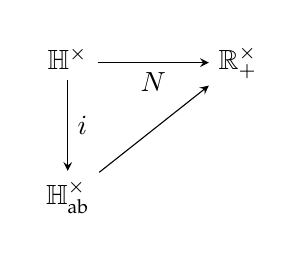
\begin{tikzpicture}
  \matrix (m) [matrix of math nodes,row sep=3em,column sep=4em,minimum width=2em]
  {
     \mathbb{H}^\times & \mathbb{R^\times_+} \\
     \mathbb{H}_\text{ab}^\times &  \\};
  \path[-stealth]
  	(m-1-1.east|-m-1-2) edge node [below] {$N$}
            node [above] {} (m-1-2)
	(m-1-1) edge node [right] {$i$} (m-2-1)
	(m-2-1) edge node [left] {} (m-1-2);
    %edge [dashed,-] (m-2-1);
	\end{tikzpicture}
    \end{minipage}
\end{figure}

Introduirem ara el determinant de Dieudonné, notem però que usant el Corol·lari \ref{mainCorollary}, ja tenim que $K_1(\mathbb{H})\cong \mathbb{R}^\times_+$.

\begin{definition}Per a tot $a\in \mathbb{H}^\times$ denotem $D(a,n)$ a la matriu invertible $n\times n$ la qual té totes les entrades iguals que la matriu identitat excepte l'entrada que ocupa la posició $(n,n)$ que té per valor $a$. Observem que 
$$
D(a)D(b)=D(ab)
$$
per a tot $a,b\in \mathbb{H}^\times$.
\end{definition}
\begin{theorem}\label{BD}
Tota matriu invertible $A$ es pot expressar de la forma $B\cdot D(\mu)$, on $B\in E(\mathbb{H})$ i $\mu \neq 0$.
\end{theorem}
\begin{proof}
La prova consisteix en aplicar transformacions elementals, segueix un procediment semblant a la prova de la Proposició \ref{K1Cos}, tots els detalls de la prova explícita es troben a [4] Teorema 4.1. 
\end{proof}
\begin{definition}
El \textbf{determinant de Dieudonné} és una aplicació 
$$
\det: GL(\mathbb{H})\rightarrow \mathbb{H}^\times_\text{ab},
$$
definit a partir del Teorema anterior, $A = BD(\mu) \mapsto \overline{\mu}$. \\
\indent A [4] s'explicita com el determinant de Dieudonné compleix (a-c) (i per tant també compleix (d-e) del Teorema \ref{bigOne} i per tant és la mateixa aplicació determinant que la descrita al Teorema \ref{bigOne}. \\
\indent Observem que el determinant de Dieudonné pren valors sobre els reals positius, de fet es comporta com el valor absolut del determinant usual de matrius reals o complexes des de tots els punts de vista (algebraic i analític).
\end{definition}
\begin{obs}
Observem que a $\mathbb{H}^\times_\text{ab}$ tenim que 
$$
\overline{ab}=\overline{a}\overline{b}=\overline{b}\overline{a}=\overline{ba}
$$
en particular, $\overline{1}=\overline{-1}$.

\end{obs}
\begin{theorem}
Si $a,b\in \mathbb{H}^\times$ i $c=aba^{-1}b^{-1}$, aleshores $D(c)$ és unimodal si $n\geq 2$.
\end{theorem}

\begin{proof}
Aquest Teorema de fet diu que si $$\overline{c}=1\in \mathbb{H}^\times_\text{ab},$$ aleshores $\det (D(c))=\overline{1}\in \mathbb{H}^\times_\text{ab}$, la prova consisteix en constatar que a partir de transformacions elementals, i.e., multiplicant per matrius de $E(\mathbb{H})$ tenim
\begin{eqnarray*}
\left( \begin{matrix}
  1 & 0 \\
  0 & 1
 \end{matrix} \right)
 &\rightarrow &
 \left( \begin{matrix}
  1 & 0 \\
  a^{-1} & 1
 \end{matrix} \right)
 \rightarrow
 \left( \begin{matrix}
  0 & -a \\
  a^{-1} & 1
 \end{matrix} \right)
 \rightarrow
 \left( \begin{matrix}
  0 & -a \\
  a^{-1} & b^{-1}
 \end{matrix} \right)
 \rightarrow
 \left( \begin{matrix}
  aba^{-1} & 0 \\
  a^{-1} & b^{-1}
 \end{matrix} \right)
 \\ &\rightarrow &
 \left( \begin{matrix}
  aba^{-1} & 0 \\
  1 & b^{-1}
 \end{matrix} \right)
 \rightarrow 
  \left( \begin{matrix}
  0 & -c \\
  1 & b^{-1}
 \end{matrix} \right)
 \rightarrow
  \left( \begin{matrix}
  0 & -c \\
  1 & c
 \end{matrix} \right)
 \rightarrow
  \left( \begin{matrix}
  1 & 0 \\
  1 & c
 \end{matrix} \right)
 \rightarrow
  \left( \begin{matrix}
  1 & 0 \\
  0 & c
 \end{matrix} \right).
\end{eqnarray*}
on cada fletxa correspon a multiplicar per una matriu de $E(\mathbb{H})$.
\end{proof}

\begin{prop}
$E(\mathbb{H})=\{A\in GL(\mathbb{H}) \ ; \ \det(A)=1\}$
\end{prop}
\begin{proof}
Està clar que tots els elements de $E(\mathbb{H})$ tenen determinant 1 , veiem la implicació no trivial, per a tota $A\in GL(\mathbb{H})$ amb $\det A = 1$ tenim que, usant el Teorema \ref{BD} $A=BD(\mu)$ amb $B\in E(\mathbb{H})$ i per tant amb determinant unimodular. Així doncs $\det A = 1$ si i només si  $\overline{\mu}=1$, per tant $\mu \in [\mathbb{H},\mathbb{H}]$, i.e., $D(\mu)\in E(\mathbb{H})$.
\end{proof}

\begin{theorem}
$K_1(\mathbb{H})\cong \mathbb{R}^\times_+$
\end{theorem}
\begin{proof}
El determinant de Dieudonné, que de fet coincideix amb el determinant del Teorema \ref{bigOne}, dóna lloc a una aplicació 
$$
\det: GL(\mathbb{H}) \rightarrow \mathbb{H}^\times_+
$$
Per la proposició anterior, tenim que $\ker (\det ) = E(\mathbb{H})$, i per tant, la factorització al abelianitzat dóna lloc a un isomorfisme $K_1(\mathbb{H})= GL(\mathbb{H})/E(\mathbb{H})\rightarrow \mathbb{H}^\times_\text{ab}$, 
\begin{center}
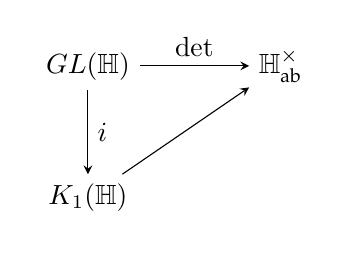
\begin{tikzpicture}
  \matrix (m) [matrix of math nodes,row sep=3em,column sep=4em,minimum width=2em]
  {
     GL(\mathbb{H}) & \mathbb{H}^\times_\text{ab} \\
     K_1(\mathbb{H}) &  \\};
  \path[-stealth]
  	(m-1-1.east|-m-1-2) edge node [above] {$\det$}
            node [above] {} (m-1-2)
	(m-1-1) edge node [right] {$i$} (m-2-1)
	(m-2-1) edge node [left] {} (m-1-2);
    %edge [dashed,-] (m-2-1);
	\end{tikzpicture}
	\end{center}
	Usant el Corol·lari \ref{HR}, on hem vist que $ \mathbb{H}^\times_\text{ab} \cong \mathbb{R}_+^\times$, trobem el que buscàvem.
\end{proof}

\section{El cas dels Dominis Euclidians.}
Al capítol anterior, en l'estudi de $K_0$, estudiàvem el cas d'un cos, el d'un DIP i el dels anells locals. En aquest capítol, en l'estudi des $K_1$ hem vist el cas d'un cos i dels anells locals, ara ens centrarem en un tipus de DIP's, els dominis Euclidians. 

\begin{definition}
Un domini d'integritat (anell no trivial sense divisors de zero) commutatiu $R$ es diu \textbf{domini Euclidià} si hi ha una funció norma $||:R\rightarrow \mathbb{N}$ amb les següents propietats:
\begin{enumerate}[i)]
\item Si $a\in R$, $|a|=0$ si i només si $a=0$.
\item Si $a,b\in R$, $|ab| = |a||b|$.
\item Si $a,b \in R$, $b\neq 0$, aleshores existeix $q,r \in R$, que anomenarem quocient i residu respectivament, els quals compleixen $a=qb+r$ i $0 \leq |r| < |b|$.
\end{enumerate}
\end{definition}

\begin{obs}
Observem que $\mathbb{Z}$, $\mathbb{Z}[i]$, $\mathbb{Z}[\frac{-1+i\sqrt{3}}{2}]$ i $K[t]$ (on $K$ és un cos) són dominis Euclidians, amb aplicacions norma definides per $|a+bi|=a^2+b^2$, $|a+b\frac{-1+i\sqrt{3}}{2}|=a^2-ab+b^2$, i per $|f(t)|=2^{\text{grau }f}$ (amb el conveni que $\text{grau} \ 0 = -\infty)$, respectivament.
\end{obs}

\begin{prop} \label{EUDesDIP}
Tot domini Euclidià és un domini d'ideals principals.
\end{prop}
\begin{proof}
Si $R$ és un domini Euclidià, l'ideal $\{0\}$ és clarament principal. Si $I$ és un ideal no nul i $b$ un element no nul d'aquest ideal tal que 
$$
|b| = \min \{ |x|, x\in I\backslash 0 \}.
$$
Aleshores existeixen $q,r \in R$ tals que $a=qb+r\in I$, amb $0\leq |r|<|b|$. Si $r\neq 0$ tenim contradicció gràcies a la tria de $b$, per tant $r=0$, i en conseqüència $I$ és un ideal principal generat per $b$.
\end{proof}

\begin{theorem}
Si $R$ és un domini Euclidià, aleshores $SK_1(R)$ és trivial i $K_1(R)\cong R^x$. De fet, per a tot $n$, $SL(n,R)=E(n,R)$.
\end{theorem}
\begin{proof}
Donada $A=(a_{ij})\in GL(n,R)$, ens agradaria usar el mateix argument que a la Proposició \ref{K1Cos}, però tenim el problema que donada una columna de $A$, no és trivial que existeixi un element invertible en aquesta columna. Considerem la primera columna de $A$, no pot passar que tots els elements siguin zero, ja que és invertible, per tant ha d'existir almenys un element no nul, assumim sense pèrdua de generalitat que $a_{i1}$ compleix la condició que és l'element amb norma mínima entre els elements no nuls d'aquesta columna. Aleshores si $|a_{i1}|=1$, per (iii) existeix una expressió $1=a_{i1}q+r$ amb $|r|<1$, per tant $|r|=0$ i tenim que $a_{i1}$ és invertible. Altrament, si $|a_{i1}|>1$, tenim que $a_{i1}$ no és invertible, i per tant genera un ideal propi $(a_{i1})$. D'altra banda com que $A$ és invertible, l'ideal generat per tots els elements de la primera columna ha de ser tot $R$, i per tant ha d'existir algun $j\neq i$ tal que $a_{j1}\not \in (a_{i1})$. Aleshores usant (iii) tenim que $a_{j1}=qa_{i1}+r$ amb $|r|<|a_{i1}|$, com que $a_{j1}\not \in (a_{i1})$ tenim que $r\neq 0$. Aleshores a partir de restar $q\times ($la fila $i$-èssima de $A)$ la la fila $j$-èssima estem fent decréixer la norma mínima dels elements no nuls de la primera columna. A partir d' iterar aquest procés, tenim una successió de valors naturals estrictament decreixent, i per tant ha de convergir a zero, i.e., aquest procediment ens permet reduir-nos al cas en que hi ha un element invertible a la primera columna. \\ Així doncs, podem transformar la matriu $A$ a la forma $$ \left( \begin{matrix}
  a_{11} & * \\
  0 & A'
 \end{matrix} \right)$$ a través de transformacions elementals per files, on $a_{11}$ és un element invertible i $A'$ una matriu invertible $(n-1)\times (n-1)$. Podem repetir aquest procés per a  $A'$, i acabar la prova amb el mateix argument usat a la Proposició \ref{K1Cos}.
\end{proof}

\begin{cor} \label{KZ}
$K_1(\mathbb{Z}) \ \cong \ \{1,-1\}$, $K_1(\mathbb{Z}[i]) \ \cong \ \{1,i, -1, -i\}$,      
 $K_1(K(x))\cong K^\times $\\ i $K_1(\mathbb{Z}[\frac{-1+i\sqrt{3}}{2}])\cong \{ z\in \mathbb{C} ; z^6 = 1\}$.
\end{cor}
\begin{proof}
Observem que per $(ii)$ tenim que si $R$ és un domini Euclidià, $a\in R$ és invertible si i només si $|a|=1$, és fàcil comprovar quins elements tenen norma 1 dels dominis Euclidians donats.
\end{proof}
\section{El grup $K_1$ relatiu i la successió exacta}
\begin{definition}
Sigui $R$ un anell (amb unitat) i $I$ un ideal bilàter de $R$. Definim el grup $K_1$ \textbf{relatiu} de l'anell $R$ i l'ideal $I$ com 
$$
K_1(R,I) = \ker ((p_1)_* : K_1(D(R,I)) \rightarrow K_1(R))
$$
Nota el paral·lelisme amb la definició \ref{K0relatiu}.
\end{definition}

\begin{definition}
Sigui $R$ un anell (amb unitat) i $I$ un ideal bilàter de $R$. Anomenarem $GL(R,I)$ al nucli de l'aplicació $GL(R)\rightarrow GL(R/I)$ induida per l'aplicació quocient $R\rightarrow R/I$. definim $E(R,I)$ com el subgrup normal de $E(R)$ més petit tal que contingui les matrius elementals $e_{ij}(a)$ amb $a\in I$.
\end{definition}

\begin{obs}
Observem que totes les matrius elementals $e_{ij}(a)$ amb $a\in I$ són congruents a la identitat a $GL(R/I)$, i per tant, $E(R,I)\subset GL(R,I)$.
\end{obs}

\begin{theorem}[Lema de Whitehead Relatiu]
Sigui $R$ un anell (amb unitat) i $I$ un ideal bilàter de $R$. Aleshores $E(R,I)$ és un subgrup normal de $GL(R,I)$ i $GL(R)$,
$$
GL(R,I)/E(R,I) \cong K_1(R,I),
$$
i $GL(R,I)/E(R,I)$ és el centre de $GL(R)/E(R,I)$. A més $E(R,I)=[E(R),E(R,I)]=[GL(R), E(R,I)]$.
\end{theorem}

\begin{proof}
Comencem veient que $E(R,I)$ és normal de $GL(R,I)$ (que és normal de $GL(R)$ ja ho hem vist al Lema de Whitehead), siguin $A\in GL(n,R)$ i $B\in E(n,R,I)$, aleshores usant la igualtat ja vista a la demostració del Lema de Whitehead tenim per una banda
$$
\left( \begin{matrix}
  ABA^{-1}B^{-1} & 0 \\
  0 & 1
 \end{matrix} \right) =  
 \left( \begin{matrix}
  AB & 0 \\
  0 & B^{-1}A^{-1}
 \end{matrix} \right)
 %
 \left( \begin{matrix}
  A^{-1} & 0 \\
  0 & A
 \end{matrix} \right)
%
 \left( \begin{matrix}
  B^{-1} & 0 \\
  0 & B
 \end{matrix} \right). 
$$
D'altra banda tenim que  $ \left( \begin{matrix}
  A^{-1} & 0 \\
  0 & A
 \end{matrix} \right)$
 és  una matriu elemental gràcies al Corol·lari \ref{matriuElemental}, a més, per la definició de $E(R,I)$ tenim que és normal de $E(R)$, i per tant, la part dreta de la igualtat anterior pertany a $E(R,I)$, provant que $E(R,I)$ és normal de $GL(R,I)$. \\
\indent Per a veure l'isomorfisme primer necessitem fer la següent observació, considerem $(A_1,A_2)\in GL(D(R,I)) \subset GL(R\times R)$ un element tal que pertany al nucli de $(p_1)_*$, i.e., aquesta aplicació l'envia a l'element identitat de $K_1(R)$ i per tant $A_1\in E(R)$, però aleshores $(A_1,A_1)\in E(D(R,I))$ ja que si $A_1=\prod_k e_{i_kj_k}(a_k)$,
 $$
 (A_1,A_1) = \prod_k e_{i_k j_k} (a_k, a_k).
 $$
Així doncs, multiplicant $(A_1, A_2)$ per $(A_1, A_1)^{-1}$ el podem transformar a la forma $(1,B)$ amb $B\in GL(R)$ sense canviar la seva classe a $K_1$. Com que $(1,B)\in GL(D(R,I))$ tenim que $B \equiv 1 \mod I$ i per tant $B\in GL(R,I)$. Recíprocament tot element $B\in GL(R,I)$ defineix una classe a $GL(D(R,I))$. Per tant, per a mostrar que $GL(R,I)/E(R,I)\cong K_1(R,I)$ només necessitem comprovar que si $B\in GL(R,I)$ aleshores $(1,B)\in E(D(R,I))$ si i només si $B\in E(R,I)$. \\
Per veure una implicació, observem que $E(R,I)$ ve generat per matrius de la forma $Se_{ij}(a)S^{-1}$ amb $a\in I$, i $S\in E(R)$. Tanmateix
$$
(1, Se_{ij}(a))S^{-1}) = (S,S) e_{ij}(0,a)(S^{-1},S^{-1})
$$
i tots els tres factors de la part dreta pertanyen a $E(D(R,I))$. Per a veure el recíproc, suposem que
$$
(1,B) = \prod_{k=1}^r e_{i_kj_k}(a_k,b_k) \in E(D(R,I)), \hspace{1cm} \prod_k e_{i_kj_k}(a_k)=1\in E(R).
$$
Observem que per a cada $k$,
$$
e_{i_kj_k}(a_k,b_k) = e_{i_kj_k}(a_k,a_k)e_{i_kj_k}(0,b_k-a_k) = (S_k,S_k)(1,T_k)
$$
on
$$
S_k = e_{i_kj_k}(a) \in E(R), \hspace{1cm} T_k=e_{i_kj_k}(b_k-a_k), \hspace{1cm} b_k-a_k \in I.
$$
Aleshores com que $S_1S_2\dots S_r =1$ tenim
\begin{eqnarray*}
\prod_k e_{i_kj_k}(a_k,b_k) &=& \\ \prod_k (S_k, S_kT_k) &=& (S1, S1T_1S_1^{-1})(S_2,S_1,S_2T_2S_2^{-1}S_1^{-1}) 
\hdots (S_r, S_1S_2\dots S_rT_r) \\
&=& (1,(S_1T_1S_1^{-1}))(S_1S_2T_sS_2^{-1}S_1^{-1}) \hdots (S_1S_2\hdots S_rT_rS_r^{-1}\hdots S_2^{-1}S_1^{-1}),
\end{eqnarray*}
i per tant, hem escrit el nostre element $B$ com a producte de generadors de $E(R,I)$. Així doncs això acaba la demostració de l'isomorfisme. \\
\indent Veiem ara darrera igualtat, com que $E(R,I)$ és un subgrup normal de $GL(R,I)$ i de $GL(R)$, tenim que  $[E(R), E(R,I)] = [GL(R), E(R,I)] \subset E(R,I)$. Per veure l'altra inclusió observem que, com que $E(R,I)$ ve generat per les matrius de la forma $Se_{ij}S^{-1}$ amb $a\in I$ i $S\in E(R)$, a més
$$
Se_{ij}(a)S^{-1} = [S,e_{ij}(a)]e_{ij}(a) = [S,e_{ij}(a)][e_{ik}(1), e_{kj}(a)] \in [E(R), E(R,I)], \ k \neq i,j.
$$
\indent Per acabar la prova hem de veure que $GL(R,I)/E(R,I)$ és el centre de $GL(R)/E(R,I)$. Veiem doncs la inclusió $G \subset Z(GL(R,I)/E(R,I))$, si $A\in GL(R,I)$ tenim que 
$$
\left( \begin{matrix}
  A & 0 \\
  0 & A^{-1}
 \end{matrix} \right) =  
 \left( \begin{matrix}
  1 & A-1 \\
  0 & 1
 \end{matrix} \right)
 %
 \left \{
 \left( \begin{matrix}
  1 & 0 \\
  1 & 1
 \end{matrix} \right)
  \left( \begin{matrix}
  1 & -A^{-1}(A-1) \\
  0 & 1
 \end{matrix} \right)
  \left( \begin{matrix}
  1 & 0 \\
  1 & 1
 \end{matrix} \right)^{-1}
%
\right \}
 \left( \begin{matrix}
  1 & 0 \\
  -(A-1) & 1
 \end{matrix} \right),
$$
i com que les entrades de $A^{-1}$ pertanyen a $I$, tenim que  les matrius 
$$
\left( \begin{matrix}
  1 & A-1 \\
  0 & 1
 \end{matrix} \right) 
 ,\hspace{1cm}
 \left( \begin{matrix}
  1 & -A^{-1}(A-1) \\
  0 & 1
 \end{matrix} \right) 
 ,\hspace{1cm} i \hspace{1cm} 
 \left( \begin{matrix}
  1 & 0 \\
  -(A-1) & 1
 \end{matrix} \right) 
$$
pertanyen a $E(R,I)$ i per tant el càlcul anterior mostra que $\left( \begin{matrix}
  A & 0 \\
  0 & A^{-1}
 \end{matrix} \right) $ pertany a $E(R,I)$. Per tant si $B\in GL(R)$, 
$$
 \left( \begin{matrix}
  ABA^{-1}B^{-1} & 0 & 0 \\
  0 & 1 & 0 \\
  0 & 0 & 0
 \end{matrix} \right)
 =
 \left[ 
 \left( \begin{matrix}
  A & 0 & 0 \\
  0 & A^{-1} & 0 \\
  0 & 0 & 1
 \end{matrix} \right)
 ,
 \left( \begin{matrix}
  B & 0 & 0 \\
  0 & 1 & 0 \\
  0 & 0 & B^{-1}
 \end{matrix} \right)
 \right] 
 \in [E(R,I), E(R)] = E(R,I).
$$ 
 per tant $GL(R,I)$ i $GL(R)$ commuten mòdul $E(R,I)$. Per a veure l'altra inclusió observem que la imatge sota el homomorfisme induït per l'aplicació quocient $R\twoheadrightarrow R/I$ del centre de $GL(R)/E(R,I)$ ha de ser el centre de $GL(R/I)$ . A més, el centre de $GL(R/I)$ és trivial ja que una matriu del centre ha de ser diagonal amb elements iguals a la diagonal, i com que una matriu qualsevol de $GL$ ha de tenir un nombre finit d'elements diferent de 1 a la diagonal, $Z(GL(S))$ és trivial.
 Per tant el centre de $GL(R)/E(R,I)$ està contingut en el nucli de l'aplicació a $GL(R/I)$, que és $GL(R,I)/E(R,I)$.
 \end{proof}

Veiem ara una extensió del Teorema \ref{K0relatiuT}.
\begin{theorem}
Sigui $R$ un anell i $I\subset R$ un ideal. Aleshores existeix una successió exacta 
\begin{equation}\label{super}
K_1(R,I) \rightarrow K_1(R) \xrightarrow{q_*} K_1(R/I) \xrightarrow{\partial} K_0(R,I) \rightarrow K_0(R) \xrightarrow{q_*} K_0(R/I),
\end{equation}
on $q_*$ ve induïda per l'aplicació quocient $q: R\twoheadrightarrow R/I$ i les aplicacions $K_j(R,I) \rightarrow K_j(R)$ venen induïdes per $p_2: D(R,I) \rightarrow R$.
\end{theorem}

\begin{proof}
Usarem la mateixa notació que al Teorema \ref{K0relatiuT} en el sentit que si $A$ és una matriu amb entrades a $R$, denotarem per $\dot{A}$ a la matriu $q(A)$, i.e. a la matriu corresponent amb entrades sobre $R/I$. \\
\indent En primer lloc veurem que la subcadena 
$$
K_1(R,I)\rightarrow K_1(R) \xrightarrow{q_*}K_1(R/I)
$$
és exacta. Per a veure-ho usarem la mateixa observació usada a la prova anterior, és a dir, usarem que tota classe de de $K_1(R,I)$ es pot representar com
$$
(1,B)\in GL(D(R,I)) \subset GL(R\times R)
$$ 
amb $B\in GL(R,I)$. Aleshores tenim que $\dot{B}=\dot{1}$ i $q_*[B]=1$ i per tant hem vist una inclusió. Per a veure l'altra inclusió considerem $B\in GL(R)$ i $q_*([B])=1$, aleshores $\dot{B}\in E(R/I)$. Ara si $\dot{a}\in R/I$, tenim que prové d'algun $a\in R$ i $e_{ij}(\dot{a})=q(e_{ij}(a))$. Per tant tot generador de $E(R/I)$ pertany a la imatge de $E(R)$ i en conseqüència $E(R/I)=q(E(R))$. (Aquest argument l'hem usat en el Lema  \ref{matrixlifting}). Per tant $\dot{B}$ ascendeix a una matriu $C\in E(R)$, i $q(BC^{-1})=1$. Aleshores $(1,BC^{-1})\in GL(D(R,I))$ i $[B]=[BC^{-1}]$ a $K_1(R)$ prové de $[(1,BC^{-1})]\in K_1(R,I)$.

\indent A continuació definirem l'aplicació frontera $K_1(R/I)\xrightarrow{\partial}K_0(R,I)$ i provarem l'exactitud de $K_1(R/I)$ i $K_0(R,I)$, un cop vist això el Teorema \ref{K0relatiuT} completarà la prova. Donada una matriu $\dot{A}\in GL(n,R/I)$, on ara $A$ $\dot{A}$ és la imatge d'una matriu $A\in M_n(R)$ no necessàriament invertible, definim
$$
R^n \times _{\dot{A}}  R^n := \{ (x,y) \in R^n \times R^n : \dot{y}=\dot{x} \dot{A} \}			
$$
pensem pensar $x$ i $y$ com a matrius $1\times n$. A la definició anterior té estructura de mòdul sobre $D(R,I)$ si imposem
$$
(r_1,r_2)\cdot (x,y) = (r_1x,r_2y).
$$
És compatible ja que, com que $\dot{r_1}=\dot{r_2}$ tenim
$$
q(r_2y)=\dot{r_2}\dot{y} = \dot{r_1}(\dot{x}\dot{A}) = q(r_1x)\dot{A}.
$$
Aquesta estructura ens permet obtenir un mòdul projectiu sobre $D(R,I)$ a partir de dos mòduls lliures. 
\\
Observem que si $\dot{A}=q(A)$ amb $A\in GL(n,R)$, aleshores
$$
(x,y)\mapsto (xA,y)\in R^n \times_i R^n \cong D(R,I)^n
$$
dóna lloc a un isomorfisme de $R^n\times_{\dot{A}} R^n$ a un mòdul lliure de rang $n$. En particular, com que hem vist que $E(R/I)=q(E(R))$, tenim que $R^n\times_{\dot{A}}R^n$ és lliure de rang $n$ si $\dot{A}$ és elemental. Per a una matriu general $\dot{A}\in GL(n,R/I)$ sempre podem escollir $\dot{B}\in GL(n,R/I)$ de forma que $\dot{A}\oplus \dot{B}$ sigui elemental (per exemple, $\dot{B}=(\dot{A})^{-1}$ funciona pel Lema \ref{matrixlifting}), i aleshores
$$
(R^n\times_{\dot{A}} R^n) \oplus (R^n \times_{\dot{B}}R^n) \cong R^{2n}\times_{\dot{A}\oplus\dot{B}}R^{2n} \cong D(R,I)^{2n},
$$
per tant $R^n \times_{\dot{A}}R^n$ és un sumand directe d'un mòdul lliure, i.e. d'un mòdul projectiu. Conseqüentment té sentit definir
$$
\partial [ \dot{A} ] := [R^n\times_{\dot{A}}R^n]-[D(R,I)^n]\in K_0(D(R,I)).
$$
\indent Veurem que $\partial$ és de fet un homomorfisme $K_1(R/I)\rightarrow K_0(R,I)$. Té imatge a $K_0(R,I)=\ker(p_1)_*$ ja que 
$$
(p_1)_*(\partial [\dot{A}] = (p_1)_*([R^n \times_{\dot{A}} R^n])
 - (p_1)_*([D(R,I)])=[R^n]-[R^n]=0$$
És additiu sota la suma directa de matrius ja que
$$
(R^n \times_{\dot{A}}) R^n) \oplus (R^n \times_{\dot{B}}) R^n) \cong R^{2n} \times_{\dot{A}\oplus \dot{B}} R^{2n}, 
$$
i envia classes de matrius elementals al $0$ ja que si $\dot{A}$ és una matriu elemental,
$$
\partial [\dot[A]] = [R^n \times_{\dot{A}} R^n] - [D(R,I)] \cong [D(R,I)^n]-[D(R,I)^n]=0.
$$
Més generalment, està ben definit sobre classes a $K_1$, ja que si $\dot{A}=\dot{BC}$ amb $B\in E(R)$, aleshores
$$
(x,y)\mapsto(xB,y)\in R^n \times_{\dot{C}}R^n
$$
dóna lloc a un isomorfisme de $R^n \times_{\dot{A}} R^n$ a $R^n\times_{\dot{C}} R^n$. Per tant obtenim un homomorfisme ben definit $K_1(R/I)\rightarrow K_0(R,I)$. A més ja hem vist que la composició
$$
K_1(R)\xrightarrow{q_*}K_1(R/I)\xrightarrow{\partial}K_0(R,I)
$$
és zero. La composició
$$
K_1(R/I)\xrightarrow{\partial} K_0(R,I) \rightarrow K_0(R)
$$
és zero ja que 
$$
(p_2)_*( \partial [\dot{A}]) = (p_2)_* ([R^n \times_{\dot{A}} R^n]) - (p_2)_*([D(R,I)^n])=[R^n]-[R^n]=0.
$$
\indent Només falta comprovar que $\ker \partial \subset q_*(K_1(R))$ i que 
$$
\ker \{ (p_2)_* : K_0(R,I) \rightarrow K_0(R) \} \subset \partial (K_1(R/I)).
$$
Suposem $\partial ([\dot{A}])=0$, això significa que $R^n\times_{\dot{A}}R^n$ és isomorf a un mòdul lliure de rang $n$, o que per alguna $m$,
$$
R^n \times_{\dot{A}}R^n \oplus D(R,I)^m \cong D(R,I)^{n+m}.
$$
Després de canviar $A$ per $A\oplus 1_m$, podem assumir que de fet
$$
R^n\times_{\dot{A}}R^n \cong D(R,I)^n.
$$
Escollim un isomorfisme 
$$
\varphi: D(R,I)^n = R^n\times_{i}R^n \rightarrow R^n \times_{\dot{A}} R^n.
$$
Aleshores podem definir les matrius $B,C\in M_n(R)$ per $(e_jB,e_jC) = \varphi(e_j,e_j)$, on $e_j$ és el $j$-èssim vector bàsic de $R^n$, en altres paraules prenem les files $j$-èssimes de $B$ i $C$ per a primera i segona coordenada de $\varphi (e_j, e_j)$. Aleshores per linealitat $\varphi (u,v) = (uB, vC)$ per a tot $(u,v)\in D(R,I)^n = R^n \times_{i}R^n$, i aleshores per a aquesta $u$ i $v$, $\dot{u}=\dot{v}$, tenim $\dot{B}\dot{A}=\dot{C}$. Per tant $\varphi$ és invertible, està clar que $B$ i $C$ són invertibles amb $\varphi(x,y)=(xB^{-1},yC^{-1})$ per $(x,y)\in R^n \times_{\dot{A}}R^n$. Per tant $\dot{A}=q(B^{-1}C)$ i per tant $\ker \partial \subset q_* (K_1(R))$. \\
\indent Finalment, suposem que tenim una classe de $K_0(R,I)$ que va a parar al $0$ de $K_0(R)$. Això significa que tenim una classe a $K_0(D(R,I))$ que va a parar al $0$ a partir de $(p_1)_*$ i de $(p_2)_*$. Representem la classe per $[P]-[D(R,I)^n]$, on $P$ és un $D(R,I)$-mòdul projectiu tal que $(p_1)_*(P)$ i $(p_2)_*(P)$ són isomorfs a $R^n$. Si és necessari, podem afegir-hi un mòdul de rang $k$ a $P$ i canviar $n$ per $n+k$ de forma que $(p_1)_*(P)$ i $(p_2)_*(P)$ siguin ambdós isomorfs a $R^n$. Aleshores està clar que $P$ és de la forma $R^n \times_{\dot{A}} R^n$, i per tant
$$
[P]-[D(R,I)^n]=\partial ([\dot{A}]).
$$
Això completa la prova.
\end{proof}


\begin{corollary}
Sigui $R$ un anell, i $I\subset R$ un ideal tal que l'aplicació quocient $q:R\rightarrow R/I$ té una inversa per la dreta, i.e., existeix un homomorfisme d'anells $s:R/I\rightarrow R$ amb $q\circ s = id_{R/I})$. Aleshores
$$
0\rightarrow K_0(I) \rightarrow K_0(R) \rightarrow K_0(R/I) \rightarrow 0
$$
és una successió exacta escindida.
\end{corollary}

\begin{proof}
Per la functorialitat de $K_0$ tenim que existeix una $s_*$ tal que $q_* \circ s_* = id_{K_0(R/I)}$. Així doncs només necessitem veure que $K_0(I)\rightarrow K_0(R)$ és injectiva. La injectivitat es veu a partir de que $s_*: K_1(R/I)\rightarrow K_1(R)$ és inversa per la dreta de $q_*:K_1(R)\rightarrow K_1(R/I)$, per tant $\partial = 0$ a la cadena exacta (\ref{super}).
\end{proof}

\begin{exemples}
Aquests darrers resultats ens proporcionen eines per a calcular $K$-grups. Veiem algúns exemples.\\
\indent Sigui $R=\mathbb{Z}$ i $I=(m)$, amb $m>0$. Recordem que al Corol·lari \ref{KZ} vem veure \\ $K_1(R)\cong \{\pm 1\}$, i a la Proposició \ref{K1Zm} hem calculat $K_1(R/I)$. Aleshores és possible calcular $K_0(I)$ a partir de la cadena exacta. Per exemple suposem $m=2$, aleshores $R/I$ és el cos format per dos elements i $(R/I)^{\times}=\{1\}$. La cadena exacta és
$$
K_1(R,I)\rightarrow \{\pm 1\} \rightarrow \{1\} \xrightarrow{\partial} K_0(I) \rightarrow \mathbb{Z} \xrightarrow{\cong} \mathbb{Z},
$$
i $K_0(I)=0$. Al mateix temps, tenim que $K_1(R,I)$ ha de ser exhaustiu a $\{\pm 1\}$.\\\\
\indent Suposem ara que $m=p$ per a $p$ primer senar. Aleshores $R/I$ és un cos $\mathbb{F}_p$ de $p$ elements i $(R/I)^{\times}$ és cyclic d'ordre $p-1$. Per tant la successió exacta esdevé
$$
K_1(R,I)\rightarrow \{\pm 1\} \rightarrow \mathbb{F}_p^{\times} \xrightarrow{\partial} K_0(I) \rightarrow \mathbb{Z} \xrightarrow{\cong} \mathbb{Z},
$$
i $K_0(I)\cong \mathbb{F}_p^{\times} \backslash \{\pm 1\}$, que és cíclic d'ordre $\frac{p-1}{2}$. En aquest cas, l'aplicació $K_1(R,I)\rightarrow \{\pm 1\}$ és trivial.
\\ \\
\indent Suposem ara que $m=2^r$ amb $r>1$. Aleshores $R/I$ és un anell local i $(R/I)^{\times}$ és un grup abelià d'ordre $2^{r-1}$.  Aleshores tenim la cadena exacta
$$
K_1(R,I)\rightarrow \{\pm 1\} \rightarrow (R/I)^{\times} \xrightarrow{\partial} K_0(I) \rightarrow \mathbb{Z}\xrightarrow{\cong} \mathbb{Z},
$$
i $K_0(I)\cong (R/I)^{\times}$ és un grup abelià d'ordre $2^{r-2}$ no necessàriament cyclic. Per exemple si $m=8$ tenim que $(R/I)^\times \cong (\mathbb{Z}/(2)\cong \mathbb{Z}/(2))$ és el 4-grup de Klein.
\end{exemples} 
%\include{Chapters/Chapter5} 

% Chapter 1

\chapter{Conclusions} 
El contingut d'aquest treball és només una petita part del que es coneix per $K$-teoria algebraica. Hem introduït els dos primers grups, els quals formen part del que es coneix per $K$-teoria algebraica clàssica. \\
\indent Per ampliar aquest treball en el sentit algebraic podríem haver estudiat $K_0$ i $K_1$ per dominis de Dedekind, aquesta estructura algebraica permet mostrar resultats interessants sobre $K$-grups. També podríem haver estudiat $K_0$ i $K_1$ per a categories en lloc d'anells, i introduir la $K$-teoria negativa. O fins i tot seria interessant estudiar el grup $K_2$. \\
\indent D'altra banda, és molt usual parlar de $K$-teoria en sentits no algebraics, cal destacar la $K$-teoria topològica, que és la branca de la topologia que es dedica a estudiar fibrats vectorials sobre espais topològics.  Ampliacions d'aquest treball en el sentit topològic poden ser interessants. \\
\indent Molts problemes profunds en àlgebra, com la classificació de subgrups normal de grups lineals, o la descripció del grup de Brauer d'un cos en termes d'àlgebres cícliques han estat resolts a través de $K$-teoria algebraica. Possibles ampliacions d'aquest treball podrien estar enfocades a estudiar aquests resultats en detall.\\
\indent Però més enllà d'això, la $K$-teoria algebraica ha aportat tècniques de resolució de problemes importants en topologia, geometria, teoria de nombres i anàlisi funcional.
En aquest treball ens hem dedicat a introduir els fonaments bàsics d'aquestes tècniques, la punta del iceberg. 
%----------------------------------------------------------------------------------------
%	THESIS CONTENT - APPENDICES
%----------------------------------------------------------------------------------------

\appendix % Cue to tell LaTeX that the following "chapters" are Appendices

% Include the appendices of the thesis as separate files from the Appendices folder
% Uncomment the lines as you write the Appendices

% Appendix A

\chapter{Conceptes de Mòduls i Estructures Algebraiques} % Main appendix title

\label{AppendixA} % For referencing this appendix elsewhere, use \ref{AppendixA}


%-----------------------------------
%	SUBSECTION 1
%-----------------------------------
L'objectiu d'aquest annex és introduir un bagatge de resultats que convé tenir presents durant la lectura del treball. El lector familiaritzat amb conceptes de mòduls pot prescindir d'aquest annex. Aquest annex permet que el treball sigui essencialment autocontingut, en el sentit que qualsevol recent graduat, estigui familiaritzat o no amb la teoria de mòduls, podrà seguir tots els conceptes exposats amb detall.\\
\indent Per la redacció de l'annex ens hem basat en [10] i [2]. 
\label{Chapter1} % Change X to a consecutive number; for referencing this chapter elsewhere, use \ref{ChapterX}

\section{Recordatori}
\begin{definition}
Un \textbf{semigrup} $(S, \cdot )$ és un conjunt amb una operació binària $\cdot : S\times S \rightarrow S$ tal que satisfà la propietat associativa, és a dir, $(a \cdot b) \cdot c = a \cdot (b \cdot c)$ per a tot $a,b,c\in S$.
\end{definition}

\begin{definition}
 Un \textbf{grup} $(G,+)$ és un conjunt $G$ amb una operació binària $+: G\times G \rightarrow G$ tal que satisfà:
\begin{itemize}
\item Associativitat: $(a+b)+c = a+(b+c)$ per a tot $a,b,c\in G$.
\item Té un elment neutre: existeix $e\in G$ tal que $e+a=a+e=a$ per tot $a\in G$.
\item Per tot $a\in G$ existeix un element invers $b\in G$ tal que $a+b=b+a=e$. \footnote{Si a l'operació binària que defineix el grup la denotem $\cdot$, a l'invers de $a$ el denotarem $a^{-1}$, de forma que $aa^{-1} = a^{-1}a = e$, en aquest cas a l'element neutre també el podem denotar per 1. Si el context permet entendre que $*$ és l'operació tal que $(G,*)$ sigui un grup, denotarem a $G$ a aquest grup. }
\end{itemize}
Diem que $(G,+)$ és un grup (o un semigrup) \textbf{commutatiu} (o abelià) si l'operació és commutativa, i.e., $a+b=b+a$ per tot $a, b\in G$. 
\end{definition}

\begin{definition} Diem que $H\subset G$ és un \textbf{subgrup} de $G$ si $H$ amb l'operació binària de $G$ és un grup. Un subgrup $N$ d'un grup $(G,\dot)$ és \textbf{normal}, i ho denotarem $N\trianglelefteq G$, si és invariant sota conjugació, és a dir, la conjugació d'un element de $N$ per un element de $G$ pertany a $N$:
$$
N\trianglelefteq G \Leftrightarrow \forall n\in N, \ \forall g\in G: \  gng^{-1}\in N
$$
\end{definition}

\begin{definition}\label{defGrupQuocient}
Sigui $N$ un subgrup normal d'un grup $(G,\cdot)$, $G/N:=\{aN: a\in G\}$. Com que $N$ és normal, si $a,b\in G$ s'ha de complir 
$$
(aN)(bN)=a(Nb)N=a(bN)N=(ab)NN=ab(N)
$$
Per tant podem estendre l'operació del grup $G$ a $G/N$ usant aquest fet, així doncs $G/N$ és un grup, que anomenem \textbf{grup quocient}.

\end{definition}

\begin{definition} Un \textbf{anell} $(R,+,\cdot )$ és un conjunt $R$ amb dues operacions binàries $+: \ R\times R \rightarrow R$ (suma) i $\cdot : R\times R \rightarrow R$ (producte) tals que satisfan:

\begin{enumerate}[a)]
\item $(R,+)$ és un grup abelià. (denotem per $0\in R$ l'element neutre).

\item $a\cdot (b \cdot c) = (a \cdot b) \cdot c$ per a tot $a,b,c\in R$ (el producte és associatiu i.e. $(R,\cdot )$ és un semigrup).
\item Té un element identitat: existeix $1\in R$ tal que $r\cdot 1=1\cdot r =r$ per tot $r\in R$.
\item $a \cdot (b+c)=a\cdot b+a \cdot c$ i $(b+c)\cdot a=b\cdot a + c\cdot a$ per a tot $a,b,c\in R$ (el producte és distributiu respecte la suma).
\end{enumerate}
Diem que $(R,+,\cdot )$ és un anell \textbf{commutatiu} si $ab=ba$ per a tot $a,b\in R$.
\end{definition}

\begin{definition}
 Un \textbf{subanell} $S$ d'un anell $R$ és un subconjunt $S$ de $R$ tal que sota les operacions suma i producte de $R$, és un anell. 
\\ \indent Per tant, $S$ és un subanell de $R$ si i només si $S$ és un subgrup additiu de $R$ tancat sota el producte. 
\end{definition}

\begin{definition} Una funció $f:R\rightarrow S$, on $R$ i $S$ són anells, és un \textbf{morfisme d'anells} si 
\begin{enumerate}[(1)]
\item $f(a+b)=f(a)+f(b)$ i $f(ab)=f(a)f(b)$ per a tot $a,b\in R$.
\item $f(1_R)=1_S$ on $1_R$ és la identitat de $R$ i $1_S$ la identitat de $S$.
\end{enumerate}
\indent De (1) es dedueix que $f(-r)=-f(r)$ i $f(0_R)=0_S$.
\\ 
\indent Donat un morfisme $f$, definim el \textbf{nucli} de $f$ com $\text{Ker}(f)=\{ r\in R : f(r)=0 \}$ i la \textbf{imatge} com $\text{Im} f = \{ x\in S : s=f(r) \ \text{per algún} \ r\in R \}$. Observem que $\text{Ker} f$ i $\text{Im}f$ són subanells de $R$ i  és un subanell de $S$ respectivament.
\\ 
\indent Si $f$ és invertible (i.e. existeix un morfisme d'anells $g:S\rightarrow R$ tal que $f \circ g =1_S$ i $g \circ f=1_R$), aleshores diem que $f$ és un \textbf{isomorfisme} d'anells, per tant $f$ és un isomorfisme d'anells si i només si és un morfisme d'anells bijectiu.
\\
A més, $f$ és injectiu si i només si $\text{Ker} f = 0$, i tautològicament, $f$ és exhaustiu si i només si $\text{Im} f=S$.
\end{definition}

\begin{definition}
Sigui $R$ un anell, diem que $I\subset R$. és un ideal de $R$ si i només si 
\begin{enumerate}[(1)]
\item $I$ és un subgrup additiu de $R$.
\item $rI\subset I$ per a tot $r\in R$
\item $Ir\subset I$ per a tot $r\in R$
\end{enumerate}
\hspace{.25cm}Un subconjunt $I\subset R$ tal que satisfaci (1) i (2) s'anomena \textbf{ideal per l'esquerra} de $R$, i similarment, si $I$ satisfà (1) i (3) s'anomena \textbf{ideal per la dreta} de $R$. Per tant un ideal de $R$ és un ideal per l'esquerra i per la dreta. \\
Diem que el ideal $I$ és \textbf{propi} si $a\subset R$ amb $a\neq R$ i $a \neq \{ 0 \}$.
\\
\hspace{.25cm}Si $R$ és commutatiu els conceptes de ideal per l'esquerra, d'ideal per la dreta i ideal són el mateix, però per anells no commutatius generalment són conceptes diferents.
\end{definition}

\textbf{Motivació de la definició d'ideal:} De teoria de grups, sabem que no tot subgrup d'un grup pot ser el nucli d'un morfisme de grups, cal que el subgrup sigui normal.  En el cas de un morfisme d'anells $f:R\rightarrow S$, $\text{Ker}(f)=\{a\in R \ : \ f(a)=0\}$ és normal ja que és subgrup respecte la suma del grup abelià $(R,+)$. \\
Observem que l'estructura multiplicativa imposa sobre l'anell $\text{Ker}(f)$ una condició més forta que la ser anell, que és la de ser ideal, és a dir, es compleix que si $a\in \text{Ker}(f)$ i $r\in R$, aleshores $f(ar)=f(a)f(r)=0f(r)=0$ i $f(ra)=f(r)f(a)=f(r)0=0$, per tant $ar\in \text{Ker}(f)$ i $ra\in \text{Ker}(f)$ per a qualsevols $a\in \text{Ker}(f)$ i $r\in R$.
\\ \\
\hspace{.25cm} \textbf{Suma d'ideals.} Observem que si $I$ i $J$ són ideals (ideal per l'esquerra, o dreta), la seva suma $I+J=\{ a+b : a \in I, \ b\in J \  \}$ és també un ideal (ideal per l'esquerra o dreta) de $R$
\\
\\
\begin{definition} Donat un ideal $I$ de $R$, diem que $r,s\in R$ són congruents mòdul $R$ si $r-a\in I$ (també es denota com $r\equiv s \text{ (mod $I$)}$. La relació de congruència és una relació d'equivalència sobre $R$. La classe de congruència es denota $\overline{r}=\{ r+x : x\in I \}$, $R/I$ és el conjunt de totes aquestes classes, definim una suma i un producte sobre $R/I$ de la forma següent: $$\overline{r}+\overline{s}=\overline{r+s},$$ $$\overline{r}\cdot \overline{s}=\overline{rs}.$$ Aleshores $R/I$ és un anell amb element neutre $\overline{0}$ i identitat $\overline{1}$. Aquest anell s'anomena \textbf{anell quocient de $R$ respecte $I$}.
\end{definition}

\noindent \textbf{Exemple.} Un exemple bàsic d'anell residu, que justifica el nom és quan considerem $R$ l'anell dels enters $\mathbb{Z}$ i $I=n\mathbb{Z}$ per algún $n>0$. Qualsevol enter $a$ pot ser escrit de la forma $a=qn+r$ amb $0\leq r <n$. L'enter $r$ és el residu i $q$ el quocient, per tant l'anell residu $\mathbb{Z}/n\mathbb{Z}$ consisteix en totes les classes de residus: $\overline{0},\overline{1},\dots, \overline{n-1}$.

\begin{theorem}[Primer teroema d'isomorfia]
Sigui $f: R \rightarrow S$ un morfisme d'anells. Aleshores $R/\text{Ker}(f) \cong \text{Im}(f)$.
\end{theorem}

\begin{theorem}[Segon teroema d'isomorfia]
Sigui $R$ un anell, $I\subset R$ un ideal i $S\subset R$ un subanell. Aleshores $S+I$ és un subanell de $R$, $I$ és un ideal de $S+I$, $S\cap I$ és un ideal de $S$, i hi ha un isomorfisme d'anells
$$
(S+I)/I \cong S/(S\cap I)
$$
\end{theorem}
\begin{theorem}[Tercer teroema d'isomorfia] Sigui $R$ un anell, siguin $I$ i $J$ ideals de $R$ tals que $I\subset J$. Aleshores $J/I$ és un ideal de $R/I$ i
$$
R/J \cong (R/I)/(J/I)
$$
\end{theorem}
\begin{theorem}[Teorema de correspondència]
Sigui $R$ un anell, $I\subset R$ un ideal de $R$ i $\pi: R \rightarrow R/I$ l'aplicació natural ($r\mapsto \overline{r}$). Aleshores la funció $S\rightarrow S/I$ defineix una correspondència bijectiva entre entre el conjunt de tots els subanells de $R$ que contenen $I$ i el conjunt de tots els subanells de $R/I$. Sota aquesta correspondència, els ideals de $R$ que contenen $I$ corresponen a ideals de $R/I$.
\end{theorem}
\begin{lemma}
 Sigui $R$ un anells i $\{S_{\alpha}\}_{\alpha \in A}$ una família de subanells (resp. ideals) de $R$. Aleshores $S=\bigcap_{\alpha \in A}S_\alpha$ és un subanell (resp. ideal) de $R$.
\end{lemma} 
\begin{proof} Sigui $a,b \in S$, aleshores existeix $a,b\in S_\alpha$ per algun $\alpha \in A$, per tant $a-b$ i $ab\in S_\alpha$, per tant $S$ és un subanell de $R$. \\
Si cada $S_\alpha$ és un ideal i $r\in R$, aleshores $ar$ i $ra\in S_\alpha$ per tot $\alpha \in A$, per tant $ar,ra\in S$ i en conseqüència $S$ és un ideal. 
\end{proof}

\begin{definition}
Sigui $R$ un anell i $X$ un subconjunt de $R$, definim el \textbf{subanell generat per $X$} com el subanell més petit de $R$ que conte $X$, similarment definim com a \textbf{ideal generat per $X$} com el ideal més petit de $R$ que contingui $X$. 
\\
Pel Lema anterior, aquest anell (resp. ideal) és la intersecció de totes els subanells (resp. ideals) que contenen $X$.  \\
Usarem la notació $\langle X \rangle$ per denotar el ideal generat per $X$.
\end{definition}

\begin{lema} Sigui $X\subset R$ un conjunt no buit de $R$.
\begin{enumerate}[(1)]
\item Si $R$ és un anell amb identitat, aleshores el ideal de $R$ generat per $X$ és el conjunt
$$
XRX= \scalebox{1.5}{\{}  \sum_{i=1}^n r_i x_i s_i : r_i ,s_i \in R , x_i\in X, n \geq 1 \scalebox{1.5}{\}} 
$$
\item Si $R$ és un anell commutatiu amb identitat, aleshores el ideal de $R$ generat per $X$ és el conjunt 
$$
RX= \scalebox{1.5}{\{}  \sum_{i=1}^n r_i x_i : r_i  \in R , x_i\in X, n \geq 1 \scalebox{1.5}{\}} 
$$
\end{enumerate}
\end{lema} 
\begin{proof} (1) tot ideal que contingui $X$ clarament ha de contenir $RXR$, només cal observar que $RXR$ és un ideal de $R$, i per tant és el ideal més petit de $R$ que conté $X$. (2) és conseqüència directa de la commutativitat de $R$.
\end{proof}

\begin{theorem}[Teorema de l'aplicació induïda (per anells)]
Sigui $f:R\rightarrow S$ un morfisme d'anells.  Aleshores existeix un únic morfisme d'anells injectiu $\overline{f}:R/ \text{Ker}f \rightarrow S$ tal que $\overline{f}\circ \pi=f$, on $\pi$ és el morfisme natural $R\rightarrow R/\text{Ker} (f)$ definit per $r\mapsto \overline{r}$.
\end{theorem}
\begin{proof}
Aquest morfisme és $\overline{f}(\overline{r})=f(r)$. El morfisme $\overline{f}$ sovint és anomenat \textbf{morfisme induït}.
\end{proof}
\begin{definition} Siguin $a\neq 0$ i $b\neq 0$ elements d'un anell $R$ tal que $ab=0$, aleshores $a$ i $b$ s'anomenen \textbf{divisors de zero} de l'anell $R$.
\end{definition}
\begin{definition} Sigui $R$ un anell, un element $a\in R$ és diu \textbf{element unitari} si té una inversa multiplicativa, és a dir, existeix $b\in R$ tal que $ab=1=ba$. Denotem per $R^*$ al conjunt d'elements unitaris de $R$.
\end{definition}
\begin{definition}
\textbf{Definició.} Un anell $R$ és un \textbf{domini de integritat} si és un anell conmutatiu tal que no té divisors de zero.
\end{definition}
\begin{definition}
\textbf{Definició.} Un anell $R$ amb identitat és un \textbf{anell de divisió} si $R^*=R \backslash \{0\}$, i.e., tot element no zero de $R$ té un invers multiplicatiu.
\end{definition}
\begin{definition}
\textbf{Definició.} Un \textbf{cos} és un anell de divisió commutatiu.
\end{definition}
\begin{definition}
\textbf{Definició.} Un grup unitari que juga un rol fonamental en $K$-teoria és el següent, donat un anell $R$ i un nombre natural $n$, el grup unitari $M_n(R)^*$ de l'anell de matrius $M_n(R)$ s'anomena grup lineal general de grau $n$, i s'escriu $GL_n(R)$.
\end{definition}

\section{Definició de Mòduls}
Els mòduls són una generalització dels espais vectorials d'àlgebra lineal, on els \textit{escalars} poden ser d'un anell arbitrari en lloc d'un cos.

\begin{definition} 
Sigui $R$ un anell. 
\begin{enumerate}
\item Un \textbf{$R$-mòdul per l'esquerra} és un grup abelià additiu $M$ amb una operació binària $\cdot : R\times M \rightarrow M$, $(r,m)\rightarrow rm$, tal que
\begin{enumerate}[$a_l$)]
\item $r(m+n)=rm+rn$
\item $(r+s)m=rm+sm$
\item $(rs)m=r(sm)$
\item $1m=m$
\end{enumerate}
Per tot $r,s\in R$ i $m,n\in M$, per a un $1\in R$.
\item Un \textbf{$R$-mòdul per la dreta} és un grup abelià additiu $M$ amb una operació binària $\cdot : M\times R \rightarrow M$, $(m,r)\rightarrow mr$, tal que
\begin{enumerate}[$a_l$)]
\item $(m+n)r=mr+nr$
\item $m(r+s)=mr+ms$
\item $m(rs)=(mr)s$
\item $m1=m$
\end{enumerate}
Per tot $r,s\in R$ i $m,n\in M$, per a un $1\in R$. 

\end{enumerate}
\end{definition}

\begin{obs}

 Si $R$ és un anell conmutatiu, aleshores qualsevol  $\tensor[_R]{M}{}$ mòdul també té estructura de $M_R$ mòdul definint $mr=rm$.
\\ \\
 Sigui $R$ un anell arbitrari, considerem $R ^{\text{op}}$, que és l'anell format pels elements de $R$, amb la mateixa suma que $R$ però amb multiplicació $\cdot $ donada per $a\cdot b = ba$. 
\\
Aleshores qualsevol $\tensor[_R]{M}{}$ mòdul és un $M_{R^\text{op}}$ mòdul.

\end{obs}

\noindent \textbf{Notació.}  Els resultats per mòduls per la dreta i per l'esquerra són paral·lels, per tant per evitar repetir els resultats, treballarem generalment amb $R$-mòduls per l'esquerra, que els denotarem \textbf{$R$-mòduls} o \textbf{mòduls sobre $R$.} \\ Si necessitem indicar per quina banda volem considerar el mòdul, denotarem per $M_R$ un $R$-mòdul per la dreta i $\tensor[_R]{M}{}$ un mòdul per l'esquerra. 

\begin{definition}
Sigui $R$ un anell i $M$, $N$ $R$-mòduls. Una aplicació $f: M\rightarrow N$ és un \textbf{homomorfisme de $R$-mòduls} si compleix
\begin{enumerate}[(1)]
\item $f(m_1+m_2)=f(m_1)+f(m_2)$ per a tot $m_1,m_2\in M$ 
\item  $f(rm)=rf(m)$ per a tot $r\in R$ i $m\in M$.
\end{enumerate}

Denotem per $\text{Hom}_R(M,N)$ a el conjunt de tots els homeomorifmes de $R$-mòduls de $M$ a $N$, si $M=N$ en lloc de homeomorfismes els podem denotar \textbf{endomorfismes}, i al conjunt d'endomorfismes d'un $R$-mòdul el denotem per $\text{End}_R(M)$. \\
Si $f\in \text{End}_R(M)$ és invertible, aleshores s'anomena \textbf{automorfisme }de $M$. El grup de tots els automorfismes  de $R$-mòduls de $M$ es denota per $\text{Aut}_R(M)$ 
\end{definition}

\begin{definition}
\begin{enumerate}[(1)]
\item Sigui $K$ un cos, aleshores un $K$-mòdul $V$ s'anomena espai vectorial sobre $K$.
\item Si $V$ i $W$ són espais vectorials sobre un cos $F$, aleshores una transformació lineal de $V$ a $W$ és un homomorfisme de $F$-mòduls de $V$ a $W$.
\end{enumerate}
\end{definition}

\textbf{Exemples}. \begin{enumerate}[(1)]
\item Un anell $R$ pot ser vist com un $R$-mòdul per la dreta (esquerra), usant la seva suma i producte d'anell com a suma i producte de mòdul per la dreta (esquerra). De forma més general, qualsevol ideal per la dreta (esquerra) de $R$ és un $R$-mòdul per la dreta (esquerra).
\item Sigui $G$ un grup abelià i $g\in G$. Si $n\in \mathbb{Z}$ definim el producte per escalars $ng$ com
$$
ng=\begin{cases}
g+\dots + g  \  \text{($n$ sumands si $n>0$)} \\
0 \ \text{si $n=0$.}\\
(-g)+\dots (-g) \  \text{($-n$ sumands si $n<0$)}
\end{cases}
$$
Usant aquest producte per escalars $G$ és un $\mathbb{Z}$-mòdul. \\
A més, si $G$ i $H$ són grups abelians i $f:G\rightarrow H$ és un homomorfisme, aleshores $f$ també és un homomorfisme de $\mathbb{Z}$-mòduls ja que per a $n>0$
$$
f(ng)=f(g+\dots g)=f(g)+\dots f(g)=nf(g)
$$
i $f(-g)=-f(g)$


\item Sigui $R$ un anell arbitrari. Aleshores $R^n$ és un $R$-mòdul, tant per la dreta com per l'esquerra, considerant el producte per escalars
\begin{eqnarray*}
a(b_1,\dots ,b_n)=(ab_1 , \dots , a_bn) \\
(b_1,\dots ,b_n)a=(b_1 a, \dots , b_n a)
\end{eqnarray*}
\item Sigui $R$ un anell, aleshores el conjunt de les matrius $M_{m,n}(R)$ és un $R$-mòdul, tant per la dreta com per l'esquerra, considerant el producte per escalars
\begin{eqnarray*}
(aA)_{i,j}=a(A)_{i,j} \\
(Aa)_{i,j}=(A)_{i,j}a
\end{eqnarray*}
\item L'aplicació producte de matrius
\begin{eqnarray*}
M_m(R) \times M_{m,n}(R)& \rightarrow  &M_{m,n}(R)\\
(A,B)&\mapsto & AB
\end{eqnarray*}
permet considerar $M_{m,n}$ com un $M_m(R)$-mòdul per l'esquerra, i similarment, la següent aplicació producte de matrius
\begin{eqnarray*}
M_{m,n}(R) \times M_{n}(R)& \rightarrow  &M_{m,n}(R)\\
(A,B)&\mapsto & AB
\end{eqnarray*}
permet considerar $M_{m,n}$ com un $M_n(R)$-mòdul per la dreta.

\item Si $R$ és un anell i $I\subset R$ un ideal, aleshores l'anell quocient $R/I$ és un $R$-mòdul tant per la dreta i per l'esquerra considerant les aplicacions producte
\begin{eqnarray*}
R \times R/I & \rightarrow & R/I \\
(a,b+I) & \mapsto & ab+I
\end{eqnarray*}
\begin{eqnarray*}
R/I \times R & \rightarrow & R/I \\
(a+I,b) & \mapsto & ab+I
\end{eqnarray*}

\item Diem que $M$ és una \textbf{$R$-àlgebra} si $M$ és un $R$-mòdul i un anell, tals que la seva suma com a anell és la mateixa que com a mòdul, i la multiplicació a $M$ i la multiplicació escalar per $R$ satisfà:
$$
r(m_1m_2)=(rm_1)m_2=m_1(rm_2)
$$
Per a cada $r\in R$, $m_1,m_2\in M$.
\begin{enumerate}
\item Tot anell és una $\mathbb{Z}$-àlgebra.
\item Si $R$ és un anell abelià, $R$ és una $R$-àlgebra.
\item Si $R$ és una anell commutatiu, aleshores l'anell de polinomis $R[X]$ i l'anell de matrius $M_n(R)$ són $R$-àlgebres.
\item Donats dos anells $R$ i $S$, i un homomorfisme d'anells $\phi: R \rightarrow S$ amb $\text{Im}(\phi)\subset Z(S):=\{a\in S : ab=ba \text{ per a tot } b\in S\}$, el centre de $S$.  Si $M$ és un $S$-mòdul, aleshores $M$ també és un $R$-mòdul usant la multiplicació escalar $am=(\phi (a))m$. \\
Com que $S$ és un $S$-mòdul, tenim que $S$ és un $R$-mòdul, a més, com que $\text{Im}(\phi)\subset C(S)$, podem concloure que $S$ és una $R$-àlgebra. 
\end{enumerate}
\item Si $M$ i $N$ són $R$-mòduls, aleshores $\text{Hom}_R(M,N)$ és un grup abelià amb la suma $(f+g)(m)=f(m)+g(m)$.\\ Si $R$ és commutatiu, podem considerar $\text{Hom}_R(M,N)$ com un $R$-mòdul definint el producte $(af)(m)=a(f(m))$. \\
Observem que imposar que $R$ sigui commutatiu és necessari per a garantir que $af$ sigui un homomorfisme de $R$-mòduls, ja que 
$$
(af)(rm)=a(f(rm))=a(r(f(m)))=ar(f(m))
$$
Només si $R$ és commutatiu podem continuar: $ar(f(m))=ra(f(m))=r(af(m))$. \\ \\
Observa també que $\text{End}_R(M)$ és a més un anell, usant la composició de homomorfismes de $R$-mòduls com a producte, i com que hi ha un homomorfisme d'anells $\phi: R\rightarrow \text{End}_R(M)$ induït per $\phi (a)=a1_M$, on $1_M$ denota el homomorfisme identitat de $M$, per l'exemple anterior (7) es dedueix que $\text{End}_r(M)$ és una $R$-àlgebra si $R$ és un anell commutatiu.
\item Si $G$ és un grup abelià, aleshores $\text{Hom}_{\mathbb{Z}}(\mathbb{Z},G)\cong G$. 
Per a veure-ho definim $\Phi: \text{Hom}_{\mathbb{Z}}  \rightarrow G $ per $\Phi (f)=f(1)$.\\
 Veiem que  $\Phi$ és un isomorfisme de $\mathbb{Z}$-mòduls: Hem de veure doncs que $\text{Ker}(\Phi)=0_M$ i que $\text{Im}(\Phi(f))=G$. 
\\ 
  El nucli només pot tenir un element, que és l'aplicació que envia tots els elements de $\mathbb{Z}$ a $0$ ja que si $f\in \text{Hom}_{\mathbb{Z}}(\mathbb{Z},G)$ es compleix per definició que $f(1)=0$, i per tant $f(n)=f(1n)=f(1)f(n)=0f(n)=0$. D'altra banda $\text{Im}(\Phi)=G$ ja que per a tot $g\in G$ existeix un homomorfisme $f$ induït per $f(1)=g$. Hem vist que $\Phi$ és bijectiu, falta veure que és un homomorfisme de $\mathbb{Z}$-mòduls. Per una banda $$\Phi(f)+\Phi(g)=f(1)+g(1)=(f+g)(1)=\Phi( f+g )$$
  D'altra banda 
  $$
  \Phi(nf)=\Phi(f+\dots +f)=(f+\dots +f)(1)=nf(1)=n\Phi (f)
  $$
  Per tant, $\Phi$ és un isomorfisme de $\mathbb{Z}$-mòduls.
  \item Generalitzant l'exemple anterior, si $M$ és un $R$-mòdul, aleshores $\text{Hom}_R(R,M)\cong M$ com a $\mathbb{Z}$-mòduls per l'aplicació $\Phi : \text{Hom}_R (R,M)\rightarrow M$ on $\Phi(f)=f(1)$.
  \item Sigui $R$ un anell commutatiu, sigui $M$ un $R$-mòdul, sigui $S\subset \text{End}_R (M)$ un subanell. Aleshores $M$ és un $S$-mòdul per la multiplicació escalar $S\times M \rightarrow M$ definida per $(f,m)\mapsto f(m)$.
  \item Sigui $T\in \text{End}_R(M)$, definim un homomorfisme d'anells $\phi : R[X] \rightarrow \text{End}_R(M)$ enviant $X$ a $T$ i $a\in R$ a $a1_M$. Per tant si 
  $$
  f(X)=a_0+a_1X+\dots + a_nX^n
  $$
  aleshores 
  $$
  \phi(f(X))=a_11_M+a_1T+\dots + a_nT^n
  $$
  Denotarem $\phi(f(X))$ per $f(T)$ i $\text{Im}(\phi)=R[T]$, és a dir, $R[T]$ és el subanell de $\text{End}_R(M)$ format pels polinomis en $T$. \\  
  Aleshores $M$ és un $R[T]$-mòdul per la multiplicació $f(T)m=f(T)(m)$. Similarment, usant el homomorfisme $\phi : R[X]\rightarrow R[T]$ tenim que $M$ és un $R[X]$-mòdul usant la multiplicació $f(X)m=f(T)(m)$.
  \\
  Aquest exemple és important, dóna la base per aplicar la teoria de mòduls sobre dominis de ideals principals per a l'estudi de transformacions lineals.
  \item Ara introduirem un exemple concret a l'exemple anterior, sigui $K$ un cos, i $T:K^2\rightarrow K^2$ una transformació lineal definida per $T(u_1,u_2)=(0,u_1)$. Tenim que $T^2=0$, per tant, si $f(X)=a_0+a_1X+\dots+a_mX^m\in K[X]$ tenim $f(T)=a_01_{K^2}+a_1T$. Per tant, l'operació producte $f(X)u$ per $u\in K^2$ ve donada per 
  $$
  f(X)\cdot (u_1,u_2)=f(T)(u_1,u_2)=(a_01_{K^2}+a_1T)(u_1,u_2)=(a_0u_1,a_0u_2+a_1u_1)
  $$
\end{enumerate}
\section{Submòduls i Quocients de Mòduls}
\begin{definition}
Sigui $R$ un anell i $M$ un $R$-mòdul. Diem que un subconjunt $N\subset M$ és un \textbf{submòdul} (o $R$-submòdul) de $M$ si $N$ és un subgrup del grup additiu $M$ i també és un $R$-mòdul usant la multiplicació escalar a $M$, és a dir, $N$ és un submòdul de $M$ si és un subgrup de $M$ tancat sota la multiplicació escalar. 
\end{definition}

\begin{lema}[Criteri de Submòdul]
Si $M$ és un $R$-mòdul i $N$ és un subconjunt de $M$ no buit, aleshores $N$ és un submòdul si i només si $x+ry\in N$ per a tot $x,y\in N$ i tot $r\in R$.
\end{lema}

\begin{definition} Si $K$ és un cos i $V$ un espai vectorial sobre $K$, un $K$-submòdul de $V$ s'anomena \textbf{subespai vectorial} de $V$.
\end{definition}
\textbf{Exemples.}
\begin{enumerate}[(1)]
\item Si $R$ és un anell, aleshores els $R$-sumbòduls del $R$-mòdul $R$ són els ideals per l'esquerra de l'anell $R$.
\item Si $G$ és un grup abelià, aleshores $G$ és un $\mathbb{Z}$-mòdul i els $\mathbb{Z}$-submòduls de $G$ són els subgrups de $G$.
\item Sigui $f:M\rightarrow N$ un homomorfisme de $R$-mòduls, aleshores $\text{Ker}(f)\subset M$ i $\text{Im}(f)\subset N$ són $R$-submòduls. \\
Es verifica usant el criteri de submòdul, en primer lloc observem que $\text{Ker}(f)$ i $\text{Im}(f)$ són conjunts no buits ja que $f(0)=0$. Si $x,y\in \text{Ker}(f)$ i $r\in R$, es compleix $f(x+ry)=f(x)+rf(y)=0$, per tant $x+ry\in \text{Ker}(f)$ i per tant $\text{Ker}(f)$ és un $R$-submòdul de $M$. D'altra banda si $x,y\in M$ i $r\in R$, tenim que $f(x)+rf(y)=f(x+ry)$ on $f(x)$ i $f(y)$ són elements arbitraris de $\text{Im}(f)$ i aplicant el criteri de submòdul queda verificat.
\item Sigui $V$ un espai vectorial sobre un cos $K$ i $T\in \text{End}_K(V)$ una transformació lineal fixada. Denotem per $V_T$ a $V$ amb l'estructura de $K[X]$-mòdul determinada per la transformació lineal $T$.\\
Aleshores un subconjunt $W\subset V$ és un $K[X]$-submòdul del mòdul $V_T$ si i nomé si $W$ és un subespai vectorial de $V$ i $T(W)\subset W$, és a dir, $W$ ha de ser un $T$-\textbf{subsepai invariant} de V. \\ \\
Per verificar-ho, observem que $X\cdot w = T(w)$ i si $a\in K$, tenim que $a\cdot w =aw$, és a dir, l'acció del polinomi constant $a\in K[X]$ sobre $V$ és la multiplicació escalar ordinaria, mentre que la acció del polinomi $X$ sobre $V$ és l'acció de $T$ sobre $V$. Per tant, un $K[X]$-submòdul de $V_T$ ha de ser un $T$-subespai invariant de $V$. \\
Recíprocament, si $W$ és un subespai vectorial de $V$ tal que $T(W)\subset W$, tenim que $T^{m}(W)\subset W$ per a tot $m\geq 1$. Per tant si $f(X)\in F(X)$ i $w\in W$ tenim $f(X)\cdot w=f(T)(w)\in W$ per tant $W$ és tancat sota la multiplicació escalar i per tant, $W$ és un $K[X]$-submòdul de $V$.
\end{enumerate}

\begin{definition}
Sigui $M$ un $R$-mòdul i $N\subset M$ un submòdul, aleshores $N$ és un subgrup d'un grup abelià $M$, per tant podem formar el quocient de grups $M/N$. Definim la multiplicació escalar del grup abelià $M/N$ per $a(m+N)=am+N$ per a tot $a\in R$ i $m+N\in M/N$.
\\ 
Com que $N$ és un $R$-submòdul de $M$, aquesta operació està ben definida, ja que si $m+N=m'+N$ tenim que $m-m'\in N$ i per tant $am-am'=a(m-m')\in N$ de forma que $am+N=am'+N$. \\
El $R$-mòdul $M/N$ considerat amb aquesta operació l'anomenem \textbf{mòdul quocient }de $M$ respecte $N$. 
\end{definition}

Ara introduirem els teoremes d'isomorfia de Noether per a
 mòduls, que són anàlegs als que hem vist per grups i anells (són conseqüència del Teorema de l'aplicació induïda).

\begin{theorem}[Primer Teorema d'isomorfia]
Sigui $M$ i $N$ mòduls sobre $R$ i $f:M\rightarrow N$ un homomorfisme de $R$-mòduls. Aleshores $$M/\text{Ker}(f)\cong \text{Im}(f)$$
\end{theorem}

\begin{proof}
pel primer Teorema d'isomorfia per a grups, tenim que existeix un isomorfisme de grups abelians $\overline{f}:M/K\rightarrow \text{Im}(f)$ definit per $\overline{f}(m+K)=f(m)$, ens falta veure que $\overline{f}$ és un homomorfisme de $R$-mòduls.  Observem que $\overline{f}(a(m+K))=\overline{f}(am+K)=f(am)=af(m)=a\overline{f}(m+K)$ per a tot $m\in M$ i $a\in R$, que és el que ens faltava veure.
\end{proof}

\begin{theorem}[Segon Teorema d'isomorfia] \label{2ntiso}
Sigui $M$ un $R$-mòdul i $N$ i $P$ submòduls. Aleshores hi ha un isomorfisme de $R$-mòduls:
$$
(N+P)/P\cong N/(N\cap P)
$$
\end{theorem}

\begin{proof} Recorda que per definició $N+P=\{n+p : n\in N, p\in P\}$. \\
Sigui $\pi : M\rightarrow M/P$ la projecció natural i $\pi_0$ la restricció de $\pi$ sobre $N$. Aleshores $\pi_0$ és un homomorfisme de $R$-mòduls amb $\text{Ker}(\pi_0)=N\cap P$ i $\text{Im}(\pi_0)=(N+P)/P$. Aplicant el primer Teorema d'isomorfia veiem el que volíem.
\end{proof}

\begin{theorem}[Tercer Teorema d'isomorfia]
Sigui $M$ un $R$-mòdul i $N$ i $P$ submòduls de $M$ amb $P\subset N$. Aleshores
$$
M/N\cong (M/P)/(N/P)
$$
\end{theorem}
\begin{proof} Definim $f: M/P\rightarrow M/N$ per $f(m+P)=m+N$, aquest homomorfisme de $R$-mòduls està ben definit i compleix
$$
\text{Ker}(f)=\{m+P : m+N=N \}=\{m+P : m\in N\}=N/P
$$
Aplicant el primer Teorema d'isomorfia queda provat.
\end{proof}

\begin{theorem}[Teorema de correspondència]
Sigui $M$ un $R$-mòdul, $N$ un submòdul i $\pi: M\rightarrow M/N$ la projecció natural. Aleshores la funció $P\rightarrow P/N$ és una correspondència bijectiva entre el conjunt de tots els submòduls de $M$ que contenen $N$ i el conjunt de tots els submòduls de $M/N$.
\end{theorem}


\section{Mòduls lliures i Bases}
\begin{definition} Sigui $R$ un anell i $S$ un subconjunt d'un $R$-mòdul $M$. Anomenem \textbf{combinació $R$-lineal} d'elements de $S$ a qualsevol element que s'expressi de la forma $$r_1s_1+\dots +r_n s_n$$ on $n$ és un enter positiu, $r_1,\dots,r_n\in R$ i $s_1,\dots s_n\in S$.\\
Denotem per a $\langle S \rangle$ al conjunt de totes les combinacions $R$-lineals d'elements de $S$, (considerem $0_M\in \langle S \rangle$ en tots els casos, encara que $S=\emptyset$). Una altra forma equivalent de pensar $\langle S \rangle $ és com la intersecció de tots els submòduls de $M$ que contenen $S$. \\
En conseqüència diem que $S$ \textbf{genera} $M$ si $\langle S \rangle =M$\\ 
\end{definition}

\begin{definition}
Sigui $R$ un anell i $S$ un subconjunt d'un $R$-mòdul $M$, una \textbf{relació $R$-lineal} de $S$ és qualsevol equació 
$$
r_1s_1+\dots +r_ns_n=0_M
$$
definida a $M$, on $n$ és un enter positiu, $s_1,\dots , s_n$ són $n$ elements diferents de $S$ i $r_1 ,  \dots , r_n$ són elements no nuls de $R$.\\
\\
Diem que el \textbf{conjunt $S$ és $R$-linealment independent} si no existeix cap relació $R$-lineal a $S$.\\
Anomenem per a \textbf{$R$-base} de $M$ a qualsevol conjunt $B\subset M$ $R$-linealment independent que generi $M$.
\end{definition}

\begin{definition}
Diem que un \textbf{$R$-mòdul} $M$ és \textbf{lliure} si té una $R$-base.
\end{definition}

\textbf{Exemples.}\begin{enumerate}[(1)]
\item Sobre qualsevol anell $R$, el mòdul zero $\{0\}$ és lliure amb el conjunt buit $\emptyset$ com a base.
\item Si $R$ és un anell no trivial, l'anell de polinomis $R[x]$ és un $R$-mòdul lliure prenent com a base d'infinits elements $\{1,x,x^2,\dots \}$.
\item Si $R$ és un anell no trivial i $n$ un enter positiu, la suma directa 
$$
R^n:=R\oplus \dots \oplus R
$$
és un $R$-mòdul lliure amb base $\{e_1, \dots , e_n\}$ on 
$$
e_i=(0,\dots 0,1,0\dots , 0)
$$
té un 1 a la coordenada $i$-èssima i $0$ a les altres. 
\\
Observem que $e_1,\dots,e_n$ generen $R^n$ ja que $(r_1,\dots, r_n)=r_1e_1+\dots+r_ne_n$, i trobar una combinació $R$-lineal entre els es elements $e_1,\dots ,e_n$ és impossible ja que si es compleix $(r_1,\dots,r_n)=(0,\dots,0)$ tenim necessàriament que $r_i=0$ per a cada $i$.
\item Sigui $R$ un anell no trivial i $S$ un conjunt no buit. Una funció $f:S\rightarrow R$ diem que té \textbf{suport finit} si $f(s)=0_R$ per a tots excepte un nombre finit de $s\in S$. \\ Denotem per  $\oplus_SR$ al conjunt de totes les funcions $f:S\rightarrow R$ amb suport finit. Sota la suma component a component i la multiplicació escalar, $\oplus_SR$ és un $R$-mòdul. \\ Si $s\in S$, denotem per $\hat{s}:S\rightarrow R$ la funció característica de $s$ definida per 
$$
\hat{s}(t)=\begin{cases}
1_R \ \text{si} \ t=s \\
0_R \ \text{si} \ t\neq s
\end{cases}
$$
El conjunt $\hat{S}=\{ \hat{s} : s\in S \}$ és una base de $\oplus_SR$ ja que si $f\in \oplus_SR$, aleshores 
$$
f=\sum_{s\in S}f(s)\hat{s}
$$
i una combinació $R$-lineal 
$$
\sum_{s\in S}f(s)\hat{s}
$$
és l'aplicació zero (= l'element zero de $\oplus_SR$) si i només si $f(s)=0_R$ per a tot $s$. \\
\\
Observem que si $S=\{ s_1,\dots , s_n\}$ té $n$ elements, existeix un isomorfisme
\begin{eqnarray*}
\oplus_SR &\rightarrow  &R^n \\
f&\mapsto &(f(s_1),\dots,f(s_n))
\end{eqnarray*}
on la base $\hat{s}_1,\dots,\hat{s}_n$, correspon a la base $e_1,\dots e_n$. \\\\
En el següent Teorema veurem que qualsevol $R$-mòdul lliure és isomorf a un de la forma $\oplus_SR$.
\end{enumerate}

\begin{theorem}
Sigui $R$ un anell i $B$ un subconjunt no buit d'un $R$-mòdul $M$. Són equivalents:
\begin{enumerate}[(i)]
\item $B$ és una $R$-base de $M$.
\item L'aplicació $R$-lineal $\phi: \oplus_BR\rightarrow M$, definida per 
$$
\phi(f)=\sum_{b\in B}f(b)b
$$
és un isomorfisme.
\item Cada $m\in M$ es pot expressar de la forma
$$
m=\sum_{b\in B}f(b)b
$$
per un i només un $f\in \oplus_BR$.
\end{enumerate} 
\end{theorem}

\begin{proof} El fet que $B$ generi $M$ equival a l'existència de l'expressió (iii) i equival a l'exhaustivitat de $\phi$. \\
El fet que $B$ sigui $R$-linealment independent, equival a la unicitat de l'expressió (iii) i equival a la injectivitat de $\phi$.
\\ \\
Els següent resultat mostra que per a definir un homomorfisme de $R$-mòduls sortint d'un mòdul lliure, és necessari i suficient especificar la imatge dels generadors. 
\end{proof}

%%%%%%%%%%%%%%%%%%%%%%%%%%%%%%%%%%%%%%%%%%%%%%%%
\begin{prop}{(Propietat universal dels $R$-mòduls lliures).} \label{morfismebase} Sigui $M$ un $R$-mòdul i $B$ un subconjunt no buit de $M$. Els següents afirmacions són equivalents:
\begin{enumerate}[(i)]
\item $B$ és una base de $M$.
\item Cada funció $\phi:B\rightarrow N$, de $B$ cap a un $R$-mòdul $N$, té una i només una extensió a una aplicació $R$-lineal $\hat{\phi}:M\rightarrow N$. \\ \\
Diem que una aplicació és $R$ lineal si compleix:
\begin{itemize}
\item $\hat{\phi}(x+y)=\hat{\phi}(x)+\hat{\phi}(y)$ per a qualsevol $x,y \in M$.
\item $\hat{\phi}(ax)=a\hat{\phi}(x)$ per a tot $a\in R$ i $x\in M$.
\end{itemize}
\end{enumerate} 
\end{prop}
%%%%%%%%%%%%%%%%%%%%%%%%%%%%%%%%%%%%%%%%%%%%%%%%

\begin{proof}
\begin{itemize}
\item (i) $\Rightarrow$ (ii): Sigui $M$ i $N$ $R$-mòduls, $B$ una base de $M$ i $\phi : B\rightarrow N$ una aplicació. Si $\hat{\phi}:M\rightarrow N$ és una aplicació $R$-lineal que exten $\phi$, cal que 
\begin{equation} \label{formula1}
\hat{\phi} \left( \sum_{b\in B}f(b)b \right)=\sum_{b\in B}f(b)\phi(b) \ \ \ \forall f\in  \oplus_BR
\end{equation}
per tant, la unicitat de l'extensió queda garantida.
\item (i) $\Leftarrow$ (ii): Considerem en particular la funció $\phi: B\rightarrow \oplus_BR$ definida per $b \mapsto \hat{b}$ per a tot $b\in B$, on $\hat{b}$ és la funció característica de l'element bàsic $b$. \\
Aplicant $\hat{\phi}$ a l'equació 
$$
\sum_{b\in B}f(b)b=0_M
$$
tenim que $f=0\in \oplus_BR$, i en conseqüència no existeix cap relació $R$-lineal a $B$. 
\\
\\
Veiem ara que $M=\langle B\rangle$: Observem que les aplicacions $f$ i la projecció $\overline{\pi}: M \rightarrow M/\langle B \rangle $ (definida per $m \mapsto \overline{m}$) envien tot $b\in B$ a $0+\langle B \rangle$. \\
Si es compleix (ii), per unicitat d'extensió $f=\overline{\pi}$ són la mateixa aplicació, per tant $M/\langle B \rangle = 0$ i $M=\langle B \rangle $.
\end{itemize}
\end{proof}

\begin{corollary}  \label{corol1}
\begin{enumerate}[(I)]
\item Si $\psi:M \rightarrow N$ és un isomorfisme de $R$-mòduls i $M$ és lliure amb base $B$, aleshores $N$ és lliure amb base $\psi(B)$.
\item  Si $M$ és un $R$-mòdul i $n$ és un enter positiu , $M$ té una base de $n$ elements si i només si $M\cong R^n$.
\item Si $M$ és un $R$-mòdul i $n$ és un enter positiu , hi ha una bijecció entre el conjunt d'isomorfismes $R^n\cong M$ cap al conjunt ordenat de bases de $n$ elements de $M$, donat per 
$$
\psi \mapsto (\psi(e_1),\dots , \psi(e_n))
$$
\end{enumerate}
\end{corollary}

\begin{proof} 
\begin{itemize}
\item
Observem que en les condicions de la proposició anterior, una extensió $R$-lineal $\hat{\phi}:M\rightarrow N$ és exhaustiva si i només si $\phi(B)$ genera $N$ , i injectiva si i només si $\phi$ és injectiva i $\phi(B)$ és linealment independent. \\
(I) és conseqüència d'aquesta constatació, considerant $\psi$ com una extensió $R$-lineal de la seva restricció a $B$.
\item (II) és conseqüència de (III). 
\item (III) Denotem per $e_1 , \dots , e_n $  una base de $R^n$. Si $\phi : R^n \rightarrow M$ és un isomorfisme, per (I) tenim que $(\psi (e_1),\dots , \psi (e_n))$ és una base ordenada de $M$. \\  Sigui $\theta : R^n \rightarrow M$ un altre isomorfisme amb $\theta (e_i) = \psi (e_i)$ per a tot $i$, aleshores constatem que són iguals:

$$
\theta \left( \sum_{i=1}^n r_ie_i \right)=
\sum_{i=1}^n r_i  \theta (e_i) =
\sum_{i=1}^n r_i \psi (e_i)
= \psi \left( \sum_{i=1}^n r_i e_i \right)
$$
L'exhaustivitat ve donada per (\ref{formula1}) i (III), ja que si considerem una base ordenada de $M$ formada per $n$ elements $(b_1 , \dots , b_n )$, aleshores existeix un isomorfisme $\psi: R^n \rightarrow M$ amb $\psi (e_i)=b_i$ per a cada $i$.

\end{itemize}
\end{proof}

El següent resultat ens permet construir a partir d'un conjunt $S$ i un anell $R$, un $R$-mòdul lliure que tingui $S$ com a base.
 
\begin{prop} 
Si $R$ és un anell no trivial, tot conjunt $S$ és base d'un $R$-mòdul lliure $F_R(S)$.
\end{prop}

\begin{proof} Si $S$ és buit, és suficient $F_R(S)=\{0_R\}$. Si $S$ és no buit, considerem el $R$-mòdul $\oplus_S R$, a l'exemple anterior hem vist que $\hat{S}$ és una base. 
 Al ser $R$ no trivial tenim que $1_R \neq 0_R$, per tant la funció $S\rightarrow \hat{S}$ definida per $s\mapsto \hat{s}$ per cada $s\in S$ és bijectiva. Usant bijectivitat podem reemplaçar $\hat{S}$ per $S$ a $\oplus_S R$. Considerem $T:=\oplus_S R - \hat{S}$, es compleix $S\cap T = \emptyset$ i per tant $h: S\cup T \rightarrow \oplus_S R$ definida per 
 $$
 h(x)=
 \begin{cases}
 x \ \text{si} \ x\in T \\
 \hat{x} \ \text{si} \ x\in S
 \end{cases}
 $$
 és una bijecció. Observem que $S\cup T$ és un $R$-mòdul sota les operacions
 \begin{eqnarray*}
 x+y &=& h^{-1}(h(x)+h(y)) \\
 rx &=& h^{-1}(rh(x))
 \end{eqnarray*}
 per $x,y\in S\cup T$ i $r\in R$. Aleshores definim $F_R(S)$ pel conjunt $S\cup T$ amb aquesta estructura de $R$-mòdul. Observem que $h$ és un isomorfisme $R$-lineal de $F_R(S)$ a $\oplus_S R$, per tant, $h^{-1}$ també és un isomorfisme $R$-lineal, i pel Corol·lari anterior (i) tenim que la base de $F_R(S)$ és $h^{-1}(\hat{S})=S$
\end{proof}


\begin{obs} Donat un conjunt $S$, podem definir un mòdul lliure que tingui $S$ com a base ($F_S(R)$), i donada una funció $\phi: S\rightarrow N$ de $S$ cap a un $R$-mòdul $N$ qualsevol, existeix una i només una extensió a una aplicació $R$-lineal $\hat{\phi}: F_S(R)\rightarrow N$.
\end{obs}

\begin{cor}
 Tot $R$-mòdul $M$ és $R$-linealment isomorf a un quocient d'un $R$-modul. Per a tot enter $n$, tot $R$-mòdul generat per a un conjunt de $n$ elements és $R$-linealment isomorf a un quocient de $R^n$.
\end{cor}


\section{Mòduls finitament generats}

\begin{definition} Un $R$-mòdul és \textbf{cíclic} si està generat per un element. Si $M$ és un $R$-mòdul i $m\in M$, el submòdul cíclic generat per $m$ és
$
\langle \{ m \} \rangle = \{ rm : r\in R \} \ ,
$
el denotem per $Rm$. \\
Un $R$-mòdul $M$ és \textbf{finitament generat} (f.g) si és generat per a un conjunt finit $\{ m_1,\dots , m_n \}$, o equivalentment, si $M$ és la suma finita de submòduls cícils:
$$
M=Rm_1+\dots +Rm_n
$$
és a dir 
$$M=\langle m_1, \dots , m_n \rangle =\text{Span} \{ m_1,\dots , m_n\}=\{0+r_1m_1+\dots +r_nm_n : r_1,\dots, r_k \in R \}$$
\end{definition}

\begin{lema} Donat un $R$-mòdul $M$ i $a_1,\dots, a_n\in M$ amb $n\in \mathbb{N}$. Tenim que $\langle a_1,\dots, a_n \rangle$ és un submòdul de $M$. 
\end{lema}

\begin{proof}  Aplicarem el criteri de submòdul, primer observem que $\langle a_1,\dots , a_n\rangle $ no és buit, ja que $0\in\langle a_1,\dots , a_n\rangle$. \\
Ara considerem $a,b\in \langle a_1,\dots , a_n\rangle$, per definició tenim que $a=r_1a_1+\dots r_na_n$ i $b=s_1a_1+\dots s_na_n$, on $r_i$ i $s_i$ són elements de $R$ per a $i=1,\dots, n$. Aleshores $a+b=(r_1+s_1)a_1+\dots +(r_n+s_n)a_n\in \langle a_1,\dots , a_n\rangle$. 
\\
Similarment si $b\in \langle a_1,\dots , a_n\rangle$ i $r\in R$, tenim que $rb=(rs_1)a_1+\dots (rs_n)a_n\in \langle a_1,\dots , a_n\rangle$. \\
Per tant, com que $a+rb\in R$, podem aplicar el criteri de submòdul i veiem el que volíem.
\end{proof}


\begin{definition} Sigui $S$ un subconjunt d'un $R$-mòdul $M$, aleshores $\langle S \rangle$ denota la intersecció de tots els submòduls de $M$ que contenen $S$. L'anomenem el \textbf{submòdul de $M$ generat per} $S$, i els elements de $S$ els anomenem \textbf{generadors} de $\langle S \rangle$
com a exemple de generació de mòdul per conjunts. \\
És a dir, $\langle S \rangle $ és el submòdul de $M$ que conté $S$ i està contingut a tot submodul $M$ que conté $S$, en altres paraules, és el submòdul més petit de $M$ que conté $S$.
\end{definition}

\textbf{Exemples. } 
\begin{enumerate}[(1)]
\item Sigui $R$ un anell, si considerem $R$ com un $R$-mòdul, tenim que $R$ com a mòdul és cíclic, i per tant finitament generat: $\langle 1 \rangle = R$.
\item Si considerem $R \oplus R$ com a $R$-mòdul veiem que és finitament generat per $\{(1,0),(0,1)\}$.
\item Tot mòdul finit és finitament generat.
\item $\mathbb{Q}$ no és finitament generat com a $\mathbb{Z}$-mòdul, veiem-ho, suposem que $\{p_1/q_1,\dots, p_n/q_n\}$ és un conjunt generador de $\mathbb{Q}$, sigui $q$ el mínim comú múltiple dels generadors ($q=\text{mcm}(q_1,\dots, q_n)$). Considerem ara $1/(q+1)$, com que $q+1$ no divideix $q$, $1/(q+1)\not \in (p_1/q_1,\dots, p_k/q_k)$ i per tant, els nombres racionals no són f.g. com a $\mathbb{Z}$-mòdul.
%http://www.math.utah.edu/~schwede/Notes/UndergradThesis.pdf
\item El concepte de $R$-mòdul generalitza el concepte de grup ciclic. De forma que, un grup abelià $G$ és cíclic (com a grup abelià) si i només si és cíclic com a $\mathbb{Z}$-mòdul.
\item Com que els $R$-submòdul $N$ de $R$ són ideals, tenim que si aquest $R$ és un $DIP$, qualsevol $R$-submòdul $N$ ha de ser cíclic.
\end{enumerate}

En un espai vectorial sobre un cos, dues bases qualsevols d'un mateix espai vectorial tenen el mateix cardinal, en un mòdul sobre un anell, de moment podem afirmar el següent:

\begin{prop} \label{prop2} Si $M$ és un $R$-mòdul lliure no finitament generat, dues bases qualsevols de $M$ tenen el mateix cardinal. 
\\
Si $M$ és un mòdul lliure f.g., aleshores tota base de $M$ és finita. 
\end{prop}

\begin{proof} Sigui $M$ un $R$-mòdul generat pel conjunt $T$, i amb base $B$; per a cada $t\in T$ existeix un subconjunt finit $B(t)\subset B$, tal que $t\in \langle B(t) \rangle $. \\
Com que $T$ genera $M$, $U:=\cup_{t\in T}B(t)$ també genera $M$ ja que per construcció $\langle T \rangle \subset \langle U \rangle \subset M$. \\
Observem que tot element de $B-U$, pertany a $M$, i $M=\langle U  \rangle$, per tant, $B=U$.
\begin{itemize}
\item Si $M$ no és finitament generat, $T$ és infinit; com que cada $B(t)$ està contingut en un conjunt numerable $\text{card}(U)\leq \text{card} (T)$, i per construcció $(U)\geq \text{card} (T)$, per tant es compleix la igualtat.
\item Si $M$ és f.g, $T$ és finit, per tant cada $B(t)$ és finit i la base $B=U$ està formada per unió finita de conjunts finits.
\end{itemize}
\end{proof}
  
 %-------------------------------------------------------
 %-------------------------------------------------------
 %-------------------------------------------------------


%\include{Appendices/AppendixB}
%\include{Appendices/AppendixC}


%%%%%%%%%%%%%%%%%%%%%%%%%%%%%%%%%%%%%%%%%%%%%%%%%%%%%%%%%%%%%%%%%%%%%%%%%%%%%%%%%%%%%%%%%

%----------------------------------------------------------------------------------------
%	BIBLIOGRAPHY
%----------------------------------------------------------------------------------------

\begin{thebibliography}{9}

\bibitem{rosenberg}
  Jonathan Rosenberg,
  \emph{Algebraic K-Theory and Its Aplications},
  Springer-Verlag New York,
  Graduate Texts in Mathematics Vol. 147
  1st edition,
  1994.

\bibitem{lamport94}
  Bruce A. Magurn,
  \emph{An Algebraic Introduction to K-Theory},
  Cambridge University Press; 1 edition,
  Encyclopedia of Mathematics and its Applications (Book 87)
  1st edition,
  2002.
   
\bibitem{markreeder}
  Mark Reeder,
  \emph{Introduction to Lie Groups},
  Department of Mathematics 
  Boston College
  \url{https://www2.bc.edu/mark-reeder/LieGroups.pdf}
  2016.
  
  %file:///C:/Users/Xavier/Downloads/[doi%2010.1002%252F9781118164518.ch4]%20Artin,%20E.%20--%20Geometric%20Algebra%20(Artin_Geometric)%20__%20The%20General%20Linear%20Group.pdf
  \bibitem{emil Artin}
  Emil Artin,
  \emph{Geometric Algebra},
  Interscience Publishers
  1957.
  
\bibitem{HelmerAslaksen}
  Helmer Aslaksen,
  \emph{Quaternionic Determinants},
  Department of Mathematics 
  National University of Singapore
  \url{http://citeseerx.ist.psu.edu/viewdoc/download?doi=10.1.1.65.877&rep=rep1&type=pdf}.
  
  \bibitem{FredRichman}
  Fred Richman,
  \emph{Non Trivial Uses of Trivial Rings},
  Proceedings of the American Mathematical Society.
  Vol 103, Number 4
  \url{http://www.ams.org/journals/proc/1988-103-04/S0002-9939-1988-0954974-5/S0002-9939-1988-0954974-5.pdf}.
  August 1988.

\bibitem{CharlesAWeibel}
  Charles A. Weibel,
  \emph{The K-book, An introduction to Algebraic K-theory},
  American Mathematical Society
  Graduate Studies in Mathematics Volume 145.
%https://books.google.es/books?id=Ja8xAAAAQBAJ&pg=PA16&lpg=PA16&dq=the+eilenberg+swindle+countably+generated+projective&source=bl&ots=Z7l-US_tQ0&sig=32yZhL2GuO9qt64zkhHtgEj8gos&hl=es&sa=X&ved=0ahUKEwiGs-y_nILPAhWGVRQKHeOBBjsQ6AEINTAD#v=onepage&q=the%20eilenberg%20swindle%20countably%20generated%20projective&f=false
  
  \bibitem{Herstein}
   I. N. Herstein,
  \emph{Non-commutative Ring Theory},
  Mathematical Association of America Textbooks
 University of Chicago
 September 2005
 Lemma 1.1.3.
 
   \bibitem{Eisenbud} 
   David Eisenbud,
  \emph{Commutative Algebra with a View Toward Algebraic Geometry},
  Springer-Verlag New York,
  Graduate Texts in Mathematics Vol. 150
 1995

   \bibitem{Adkins} 
   William A. Adkins, Steven H. Weintraub
  \emph{Algebra},
  Springer-Verlag,
  Graduate Texts in Mathematics Vol. 136
 1992
%@book{book:4866,
%   title =     {Algebras, Rings and Modules},
%   author =    {Michiel Hazewinkel, Nadiya Gubareni, V.V. Kirichenko},
%   publisher = {Springer},
%   isbn =      {1402051409,9781402051401,9781402051418},
%   year =      {2007},
%   series =    {Mathematics and Its Applications},
%   edition =   {1},
%   volume =    {Volume 2},
%   url =       {http://gen.lib.rus.ec/book/index.php?md5=997C4A1312B45B305A7CA36181803771}}

%"commutator"
%http://isites.harvard.edu/fs/docs/icb.topic731509.files/Homework_4_Benjamin_Dozier_Solutions.pdf
\end{thebibliography}
%----------------------------------------------------------------------------------------

\end{document}  
